% !TEX program = pdflatex
% !TEX encoding = UTF-8 Unicode

% Plantilla, basada en la clase `scrbook` del paquete KOMA-script,  para la elaboración de un TFG siguiendo las directrices del la comisión del Grado en Matemáticas de la Universidad de Granada.

% Francisco Torralbo Torralbo

\documentclass[print, color]{ugrTFG}

% VERSIÓN ELECTRÓNICA PARA TABLETA
% Cambiando la opción "print" por "tablet" generaremos un pdf adaptado para leerlo en tabletas de 9 pulgadas.

% -------------------------------------------------------------------
% INFORMACIÓN DEL TFG Y EL AUTOR
% -------------------------------------------------------------------

\newcommand{\miTitulo}{Título del trabajo\xspace}
\newcommand{\miNombre}{Isabel María Moreno Cuadrado\xspace}
\newcommand{\miGrado}{Doble Grado en Matemáticas e Ingeniería Informática}
\newcommand{\miFacultad}{Facultad de Ciencias y Facultad de la ETSIIT \textbf{(falta logo)}}
\newcommand{\miUniversidad}{Universidad de Granada}

% Añadir tantos tutores como sea necesario separando cada uno de ellos mediante el comando `\medskip` y una línea en blanco
\newcommand{\miTutor}{
  Nombre del tutor 1 \\ \emph{Departamento del tutor 1} 

  % Añadir tantos tutores como sea necesario. 

  \medskip
  Nombre del tutor 2 \\ \emph{Departamento del tutor 2}
}
\newcommand{\miCurso}{2023-2024\xspace}

\hypersetup{
	pdftitle={\miTitulo},
	pdfauthor={\textcopyright\ \miNombre, \miFacultad, \miUniversidad}
}


\usepackage{upgreek}

\usepackage{accents}
\usepackage{pgfplots}
\usepackage{amsmath}
\usepackage{amsfonts}
\usepackage{amssymb}
\usepackage{mathtools}
\usepackage{algorithm}
\usepackage{algpseudocode}
\usepackage{mathrsfs}
\usepackage{enumitem}
\usepackage{csquotes}
\usepackage{amsthm} % Para utilizar el comando \qedhere

\begin{document}

\maketitle

% -------------------------------------------------------------------
% FRONTMATTER
% -------------------------------------------------------------------
\frontmatter % Desactiva la numeración de capítulos y usa numeración romana para las páginas

% !TeX root = ../tfg.tex
% !TeX encoding = utf8
%
%*******************************************************
% Declaración de originalidad
%*******************************************************

\thispagestyle{empty}

\hfill\vfill

\textsc{Declaración de originalidad}\\\bigskip

D./Dña. \miNombre \\\medskip

Declaro explícitamente que el trabajo presentado como Trabajo de Fin de Grado (TFG), correspondiente al curso académico \miCurso, es original, entendido esto en el sentido de que no he utilizado para la elaboración del trabajo fuentes sin citarlas debidamente.
\medskip

En Granada a \today 
\vspace{3cm}
\begin{center} 
Fdo: \miNombre 

\end{center}

\vfill

\cleardoublepage
\endinput
   
% !TeX root = ../tfg.tex
% !TeX encoding = utf8

%*******************************************************
% Dedication
%*******************************************************
\thispagestyle{empty}
\phantomsection 
\pdfbookmark[1]{Dedicatoria}{Dedicatoria}

\hfill
\vfill

\begin{flushright}
\itshape
Dedicatoria (opcional) \\
Ver archivo \texttt{preliminares/dedicatoria.tex}
\end{flushright}

\vfill

\cleardoublepage
\endinput
                % Opcional
% !TeX root = ../tfg.tex
% !TeX encoding = utf8

%*******************************************************
% Table of Contents
%*******************************************************
\phantomsection
\pdfbookmark[0]{\contentsname}{toc}

\setcounter{tocdepth}{2} % <-- 2 includes up to subsections in the ToC
\setcounter{secnumdepth}{3} % <-- 3 numbers up to subsubsections

\tableofcontents 

%*******************************************************
% List of Figures and of the Tables
%*******************************************************

    % *******************************************************
    %  List of Figures
    % *******************************************************    
    \phantomsection 
    % \listoffigures

    %*******************************************************
    % List of Tables
    %*******************************************************
    \phantomsection 
    % \listoftables
    
    %*******************************************************
    % List of Listings
    % The package \usepackage{listings} is needed
    %*******************************************************      
	  % \phantomsection 
    % \renewcommand{\lstlistlistingname}{Listados de código}
    % \lstlistoflistings 

\cleardoublepage
            
% !TeX root = ../tfg.tex
% !TeX encoding = utf8

%*******************************************************
% Agradecimientos
%*******************************************************

\chapter{Agradecimientos}

Agradecimientos (opcional, ver archivo \texttt{preliminares/agradecimiento.tex}).

\cleardoublepage
\endinput
            % Opcional

% !TeX root = ../tfg.tex
% !TeX encoding = utf8
%
%*******************************************************
% Summary
%*******************************************************

\selectlanguage{english}
\chapter{Summary}

An english summary of the project (around 800 and 1500 words are recommended).

File: \texttt{preliminares/summary.tex}


% Al finalizar el resumen en inglés, volvemos a seleccionar el idioma español para el documento
\selectlanguage{spanish} 
\endinput
                    
% !TeX root = ../tfg.tex
% !TeX encoding = utf8
%
%*******************************************************
% Introducción
%*******************************************************

% \manualmark
% \markboth{\textsc{Introducción}}{\textsc{Introducción}} 

\chapter{Introducción}

\noindent Al aplicar la transformada de Fourier a una señal en el dominio del tiempo, obtenemos su representación en el dominio de la frecuencia. Esto nos permite examinar la señal original como una composición en términos de componentes sinusoidales.

\noindent Una imagen no es más que una señal visual, y es así susceptible de ser representada en el dominio de la frecuencia. Allí, trabajando con la magnitud y la fase, no solo podremos recuperar la imagen original, sino que ciertas tareas como extracción de características, compresión o  eliminación de ruido, se verán significativamente simplificadas.

\noindent Dado que partimos de datos discretos, y que los ordenadores solo pueden manejar sumas finitas, surge la  imperiosa necesidad de definir en este ambiente una 'aproximación' de la transformada de Fourier.


\noindent \textbf{Completar al final del trabajo.}


\endinput
               

% -------------------------------------------------------------------
% MAINMATTER
% -------------------------------------------------------------------
\mainmatter % activa la numeración de capítulos, resetea la numeración de las páginas y usa números arábigos

\part{Parte Matemática} % Dividir un TFG en partes 

% !TeX root = ../tfg.tex
% !TeX encoding = utf8
%
%*******************************************************
% Introducción
%*******************************************************

% \manualmark
% \markboth{\textsc{Introducción}}{\textsc{Introducción}} 
\chapter{Introducción}
 hablar sobre quien es $L^1(\mathbb{R}^n)$ y definir traslacion y mu  y todo eso  quizas es mejor en otro capitulo ns 
\chapter{Preliminares}

De ahora en adelante trabajaremos con el espacio vectorial $\mathbb{R}^n$. En este espacio definimos el producto escalar de dos vectores \( x = (x_1, x_2, \ldots, x_n) \in \mathbb{R}^n \) e \( y = (y_1, y_2, \ldots, y_n) \in \mathbb{R}^n \) como el número real $\langle x, y \rangle$ dado por

\begin{equation}\label{eq:prod}
    \langle x, y \rangle = \sum_{k=1}^{n} x_k y_k.
\end{equation}
 
\noindent El espacio $\mathbb{R}^n$ dotado del producto escalar definido en~\eqref{eq:prod} es un espacio de Hilbert, que se conoce como el espacio euclídeo $n$-dimensional. 

\noindent La norma asociada a
dicho producto escalar es la norma euclídea $||\cdot||_2$. El espacio euclídeo $n$-dimensional es un espacio normado con esta norma. En $\mathbb{R}^n$ es posible considerar otras normas distintas. Sin embargo, en ausencia de especificación, se presume el uso de la norma euclídea.

\noindent El espacio $\mathbb{R}^n$ es además un espacio topológico con la topología usual que es la generada por la distancia asociada a la norma en $\mathbb{R}^n$. Es indiferente que norma se considere ya que todas ellas son equivalentes.


\section{Espacios $\mathscr{L}^p(\mathbb{R}^n)$}

\noindent Sea $\mathscr{L}^0(\mathbb{R}^n) = \{f: \mathbb{R}^n \rightarrow \mathbb{C}\ : \  f \ \text{es medible}\}$. Para cada $p \in \mathbb{R}$ con $p \geq 1$, se define
\begin{equation}
    \mathscr{L}^p(\mathbb{R}^n) = \left\{ f \in \mathscr{L}^0(\mathbb{R}^n): \int_{\mathbb{R}^n} |f(x)|^p \, dx < \infty \right\},
\end{equation}

\noindent y para cada función $f \in \mathscr{L}^p(\mathbb{R}^n)$, se define la seminorma
\begin{equation}
    ||f||_p = \left( \int_{\mathbb{R}^n}|f(x)|^p  \, dx \right)^{\frac{1}{p}}.
\end{equation}

\noindent Definimos también 
\begin{equation}
    \mathscr{L}^{\infty}(\mathbb{R}^n) = \{f \in \mathscr{L}^{0}(\mathbb{R}^n): f \, \text{está esencialmente acotada en}\, \mathbb{R}^n\},
\end{equation}

\noindent y, dada una función $f \in \mathscr{L}^\infty(\mathbb{R}^n)$, se define
\begin{equation}
    ||f||_\infty = \inf\{M \in [0, \infty[\,: |f(x)|\leq M \, \text{c.p.d. en}\, \mathbb{R}^n\}.
\end{equation}

\noindent Para cada $1 \leq p \leq \infty$, el espacio $L^p(\mathbb{R}^n)$ es el espacio de Banach originado por la identificación en $\mathscr{L}^p(\mathbb{R}^n)$ de las funciones que coinciden casi por doquier.
Por lo que los elementos de $L^p(\mathbb{R}^n)$ no son funciones sino clases de funciones bajo la relación
de equivalencia de “ser iguales casi por doquier”. 

\noindent El espacio \( L^2(\mathbb{R}^n) \) es digno de atención especial, siendo un espacio de Hilbert cuyo producto escalar se define mediante la fórmula
\begin{equation}
    \langle f,g \rangle = \int_{\mathbb{R}^n}f(x)\overline{g(x)}\, dx \quad \forall f,g \in  L^2(\mathbb{R}^n).
\end{equation}

\begin{proposicion}
    Sea \(f,g \in L^2(\mathbb{R}^n)\). Se verifica la  identidad
    \begin{equation}
         \langle f,g \rangle = \frac{1}{4} \left[ ||f+g||_2^2 - ||f-g||_2^2 + i||f+ig||_2^2 - i||f-ig||_2^2 \right].
    \end{equation}
denominada identidad de polarización.
\end{proposicion}


\begin{proposicion} \label{prop:inco}
Los espacios $\mathscr{L}^p(\mathbb{R}^n)$ son mutuamente incomparables. 
\end{proposicion}
\begin{proof}
    Sea $1 \leq p < q \leq \infty$. Fijamos $p < a < q$ y definimos la siguiente función $f: \mathbb{R}^n \rightarrow \mathbb{R}$ como
    \begin{equation}
        f(x) = \begin{cases}
    \prod_{i=1}^n x_i^{-1/a} & \text{si } x_i > 1 \, \, \forall i \in \{1,\ldots, n\}, \\
    0 & \text{en otro caso. } 
\end{cases}
    \end{equation}
Entonces se tiene que $f \notin \mathscr{L}^p(\mathbb{R}^n)$ y $f \in \mathscr{L}^q(\mathbb{R}^n)$.

\noindent Por otro lado definimos $g: \mathbb{R}^n \rightarrow \mathbb{R}$  como
 \begin{equation}
        f(x) = \begin{cases}
    \prod_{i=1}^n x_i^{-1/a} & \text{si } 0< x_i < 1 \, \, \forall i \in \{1,\ldots, n\}, \\
    0 & \text{en otro caso. } 
\end{cases}
\end{equation}

\noindent Es claro que $f \notin \mathscr{L}^q(\mathbb{R}^n)$ y $f \in \mathscr{L}^p(\mathbb{R}^n)$.

\noindent Concluimos entonces que   los conjuntos $\mathscr{L}^q(\mathbb{R}^n)$ y $\mathscr{L}^p(\mathbb{R}^n)$ son incomparables:
$\mathscr{L}^q(\mathbb{R}^n) \not\subset \mathscr{L}^p(\mathbb{R}^n)$ y $\mathscr{L}^p(\mathbb{R}^n) \not\subset \mathscr{L}^q(\mathbb{R}^n)$.
\end{proof}

\begin{proposicion}
Sea $f\in \mathscr{L}^1(\mathbb{R}^n)$. Entonces, para cada $t \in \mathbb{R}^n$, la función $x \mapsto f(x-t)$ es integrable en $\mathbb{R}^n$ y se cumple la identidad
\begin{equation}
    \int_{\mathbb{R}^n}f(x-t) \, dx = \int_{\mathbb{R}^n}f(x)\, dx.
\end{equation}
\end{proposicion}


\noindent Definimos otros dos espacios con los que también trabajaremos.
\begin{definicion}
    El conjunto $C_{0}(\mathbb{R}^n)$ es el conjunto de las funciones continuas $f: \mathbb{R}^n \rightarrow \mathbb{C}$ que se anulan en infinito.
\end{definicion}
\begin{definicion}
    El conjunto $C_{00}(\mathbb{R}^n)$ es el conjunto de las funciones continuas $f: \mathbb{R}^n \rightarrow \mathbb{C}$ cuyo soporte es compacto.
\end{definicion}
\begin{proposicion}
    $C_{0}(\mathbb{R}^n)$ es un espacio normado con la norma 
    \begin{equation}
        ||f||_\infty = \max\{|f(x)|: x \in \mathbb{R}^n\} ,\quad \forall f \in C_{0}(\mathbb{R}^n).
    \end{equation}
    y se tiene que  $C_{00}(\mathbb{R}^n)$ es un subespacio denso en $C_{0}(\mathbb{R}^n)$.
\end{proposicion}


\noindent Para $ 1 \leq p \leq \infty$, se tiene que $C_{00}(\mathbb{R}^n) \subset \mathscr{L}^p(\mathbb{R}^n) $. De hecho, sabemos que $C_{00}(\mathbb{R}^n)$ es denso en $\mathscr{L}^p(\mathbb{R}^n)$. 
\begin{teorema}\label{teo:sc}
    Sea $1 \leq p < \infty$ y sea $f \in \mathscr{L}^p(\mathbb{R}^n)$. Entonces para cada $\epsilon \in \mathbb{R}^+$, existe $g \in C_{00}(\mathbb{R}^n)$ tal que $||f-g||_p < \epsilon$.
\end{teorema}

\section{Definiciones}

 \begin{definicion}
    Sea $f \in \mathscr{L}^0(\mathbb{R}^n)$, para cada $a \in \mathbb{R}^+$, definimos $H_af \in \mathscr{L}^0(\mathbb{R}^n) $ como $H_af(x)=f(ax).$
\end{definicion}
\begin{proposicion}
    Para $ 1\leq p \leq \infty$, sea $f \in \mathscr{L}^p(\mathbb{R}^n)$. Entonces, para cada $a \in \mathbb{R}^+$,  $H_af \in \mathscr{L}^p(\mathbb{R}^n) $ y $||H_af||_p = a^{-n/p}||f||_p$.
\end{proposicion}

\begin{proof}
Sea $ 1\leq p < \infty$, y $a \in \mathbb{R}^+$. Usaremos que $f \in \mathscr{L}^p(\mathbb{R}^n)$. Entonces realizando un cambio de variable adecuado se tiene que
\begin{equation}
       \int_{\mathbb{R}^n} |H_af(x)|^p  \, dx =\int_{\mathbb{R}^n} |f(ax)|^p  \, dx =  a^{-n}\int_{\mathbb{R}^n} |f(x)|^p  \, dx = a^{-n}||f||_p^p< \infty.
\end{equation}
    
\noindent De donde se deduce que $||H_af||_p = a^{-n/p}||f||_p$.
\vspace{0.2cm}

\noindent Para $p= \infty$, se tiene que $f$ está esencialmente acotada en $\mathbb{R}^n$. Entonces, 
  como $|H_af(x)|^p= |f(ax)|  \,\, \forall x \in \mathbb{R}^n$, se tiene que $\tau_t{f}$ está esencialmente acotada en $\mathbb{R}^n$ y  el supremo esencial coincide evidentemente en ambos casos.
\end{proof}




\begin{definicion}
Sea $f \in \mathscr{L}^0(\mathbb{R}^n)$. Para cada $t \in \mathbb{R}^n$, definimos 
\begin{itemize}
    \item $\tau_tf \in \mathscr{L}^0(\mathbb{R}^n) $ como $\tau_tf(x)=f(x-t) \,\,\forall x \in \mathbb{R}^n,$
    \item $\mu_tf \in \mathscr{L}^0(\mathbb{R}^n) $ como $\mu_tf(x)=e^{2 \pi i  \langle x, t \rangle}f(x) \,\, \forall x \in \mathbb{R}^n$.
\end{itemize}
\end{definicion}

\begin{proposicion}
    Para $ 1\leq p \leq \infty$, sea $f \in \mathscr{L}^p(\mathbb{R}^n)$. Entonces, para cada  $t \in \mathbb{R}^n$,  $\tau_tf,\mu_tf \in \mathscr{L}^p(\mathbb{R}^n) $ y $||\tau_tf||_p = ||\mu_tf||_p = ||f||_p$.
\end{proposicion}
\begin{proof}
Sea $ 1\leq p < \infty$, y $t \in \mathbb{R}^n$. Entonces
    \begin{equation}
       \int_{\mathbb{R}^n} |\tau_tf(x)|^p  \, dx =\int_{\mathbb{R}^n} |f(x-t)|^p  \, dx =  \int_{\mathbb{R}^n} |f(x)|^p  \, dx = ||f||_p^p< \infty,
    \end{equation}
    \begin{equation}
        \int_{\mathbb{R}^n} |\mu_tf(x)(x)|^p  \, dx = \int_{\mathbb{R}^n} |e^{2 \pi i  \langle x, t \rangle}f(x)|^p  \, dx= \int_{\mathbb{R}^n} |f(x)|^p  \, dx = ||f||_p^p< \infty.
    \end{equation}
De donde se deduce que $||\tau_tf||_p = ||\mu_tf||_p = ||f||_p$.
\vspace{0.2cm}

\noindent Para $p= \infty$, se tiene que $f$ está esencialmente acotada en $\mathbb{R}^n$. Entonces, 
\begin{itemize}
    \item   Como $|\tau_t{f}(x)| = |f(x-t)| = |f(x)| \quad \forall x \in \mathbb{R}^n$, se tiene que $\tau_t{f}$ está esencialmente acotada en $\mathbb{R}^n$.
    \item Como $|\mu_t(x)| = |e^{2 \pi i  \langle x, t \rangle}f(x)|= |f(x)|  \quad \forall x \in \mathbb{R}^n$, se sigue que $\mu_t{f}$ está esencialmente acotada en $\mathbb{R}^n$.
\end{itemize} 
Además, el supremo esencial coincide evidentemente en los tres casos.
\end{proof}

\begin{definicion}
Sea $f \in \mathscr{L}^0(\mathbb{R}^n)$, definimos 
\begin{itemize}
    \item $\overline{f} \in \mathscr{L}^0(\mathbb{R}^n) $ como $\overline{f}(x)=\overline{f(x)} \quad \forall x \in \mathbb{R}^n,$
    \item $\widetilde{f} \in \mathscr{L}^0(\mathbb{R}^n) $ como $\widetilde{f}(x)=f(-x) \quad \forall x \in \mathbb{R}^n.$
\end{itemize}
\end{definicion}

\begin{proposicion} \label{prop:conj}
    Para $ 1\leq p \leq \infty$, sea $f \in \mathscr{L}^p(\mathbb{R}^n)$. Entonces,   $\overline{f},\widetilde{f} \in \mathscr{L}^p(\mathbb{R}^n) $, y $||\overline{f}||_p = ||\widetilde{f}||_p = ||f||_p$.
\end{proposicion}

\begin{proof}
Sea $ 1\leq p < \infty$. Entonces
    \begin{equation}
       \int_{\mathbb{R}^n} |\overline{f}(x)|^p  \, dx =  \int_{\mathbb{R}^n} |\overline{f(x)}|^p  \, dx = \overline{\int_{\mathbb{R}^n} |f(x)|^p  \, dx} = ||f||_p^p< \infty,
    \end{equation}
    \begin{equation}
        \int_{\mathbb{R}^n} |\widetilde{f}(x)|^p  \, dx = \int_{\mathbb{R}^n} |f(-x)|^p  \, dx= ||f||_p^p< \infty.
    \end{equation}
De donde se deduce que $||\overline{f}||_p = ||\widetilde{f}||_p = ||f||_p$.
\vspace{0.2cm}

\noindent Para $p= \infty$, se tiene que $f$ está esencialmente acotada en $\mathbb{R}^n$. Entonces, 
\begin{itemize}
    \item   Como $|\widetilde{f}(x)| = |f(-x)| \,\, \forall x \in \mathbb{R}^n$, se tiene que $\widetilde{f}$ está esencialmente acotada en $\mathbb{R}^n$.
    \item Como $|\overline{f}(x)| = |\overline{f(x)}|= |f(x)|  \,\, \forall x \in \mathbb{R}^n$, se sigue que $\overline{f}$ está esencialmente acotada en $\mathbb{R}^n$.
\end{itemize} 
Además, el supremo esencial coincide evidentemente en los tres casos.
\end{proof}

\noindent Estos resultados se usarán en adelante sin hacer mención explícita a ellos. 

\section{Módulo de Continuidad}
\begin{definicion}
Sea $1\leq p < \infty$ y sea $f \in \mathscr{L}^p(\mathbb{R}^n)$. El \textit{módulo de continuidad en media} de $f$ es la función $w_pf: \mathbb(\mathbb{R}^n) \rightarrow \mathbb{R}$ definida por 
\begin{equation}
    w_pf(t) =||\tau_tf-f||_p  \quad \forall t \in \mathbb{R}^n.
\end{equation}
\end{definicion}

\begin{proposicion}\label{mod_cont}
Sea $1\leq p < \infty$ y sea $f \in \mathscr{L}^p(\mathbb{R}^n)$. Entonces, 
\begin{itemize}
    \item $w_pf(t)=w_pf(-t) \quad \forall t \in \mathbb{R}^n$,
    \item $0 \leq w_pf(t)  \leq 2||f||_p \quad \forall t \in \mathbb{R}^n$,
    \item $w_pf$ es uniformemente continua en $\mathbb{R}^n$. En particular, $\underset{\substack{t \rightarrow 0}}{\lim}w_pf(t)=0.$
\end{itemize}
\end{proposicion}
\begin{proof}
Comenzamos probando la simetría de $w_pf$. Para ello, tomamos $t \in \mathbb{R}^n$, y observamos que:
\begin{equation}
    w_pf(t) = \left(\int_{\mathbb{R}^n} |f(x-t)-f(x)|^p dx\right)^{\frac{1}{p}} = \left(\int_{\mathbb{R}^n} |f(y)-f(y+t)|^p dy\right)^{\frac{1}{p}}=w_pf(-t).
\end{equation}
Continuamos observando que, en efecto, $0 \leq w_pf(t)$. Para la otra acotación, tomando $t \in \mathbb{R}^n$:
\begin{equation}
     w_pf(t) =||\tau_tf-f||_p \leq 2 ||f||_p.
\end{equation}
A continuación, probamos que $w_pf$ es uniformemente continua. 
Lo que haremos será utilizar el Teorema \ref{teo:sc}.

\noindent Dado $\epsilon \in \mathbb{R}^+$, existe una función $g$ continua con soporte compacto tal que $||f-g||_p < \frac{\epsilon}{3}$.

\noindent Como la función $g$ es continua con soporte compacto, sabemos que existe $R>0$, tal que $\{x \in \mathbb{R}^n : g(x) \neq 0\} \subset B_{||\cdot||_\infty}(0,R)$. Además, al ser g uniformemente continua, existe $0 < \delta <1$ tal que
\begin{equation}\label{eq:acot}
    x,y \in \mathbb{R}^n, |x-y| < \delta \implies |g(x)-g(y)| < \frac{\epsilon}{3M^{\frac{1}{p}}}\,,
\end{equation}
con $M = \mu({B_{||\cdot||_\infty}(0,R+1)})$ donde $\mu$ es la medida de Lebesgue.

\noindent Para cada $s,t \in \mathbb{R}^n$, tenemos que
\begin{equation}
    |w_pf(s)-w_pf(t)| \leq ||(\tau_sf-f)-(\tau_tf-f)||_p = ||\tau_sf-\tau_tf||_p.
\end{equation}
Usando la función $g$ podemos escribir
\begin{align}
||\tau_sf-\tau_tf||_p &= ||\tau_sf-\tau_tf +g -g + \tau_sg -\tau_sg +\tau_tg -\tau_tf || \\
&= ||\tau_s(f-g)+(\tau_sg-\tau_tg) - \tau_t (f-g)||_p 
\leq 2 ||f-g||_p + ||\tau_sg-\tau_tg||_p.
\end{align}
Tratamos entonces de acotar el segundo término. Tomamos $|s-t| < \delta $. Usando~\eqref{eq:acot} y teniendo en cuenta que $g(x-(s-t))=g(x) = 0 \,\, \forall x \notin B_{||\cdot||_\infty}(0,R+1)$, se tiene que 
\begin{equation}
    ||\tau_sg-\tau_tg||_p = \left( \int_{\mathbb{R}^n}|g(x-(s-t))-g(x)|^{p} \, dx\right)^{\frac{1}{p}} \leq \left( \int_{B_{||\cdot||_\infty}(0,R+1)}\left|\frac{\epsilon}{3M^{\frac{1}{p}}}\right|^p \, dx\right)^{\frac{1}{p}} \leq \frac{\epsilon}{3}.
\end{equation}

\noindent Deducimos finalmente que 
\begin{equation}
    |w_pf(s)-w_pf(t)|\leq 2 ||f-g||_p + ||\tau_sg-\tau_tg||_p \leq \epsilon.
\end{equation}


\noindent Luego $w_pf$ es uniformemente continua en $\mathbb{R}^n$. Si tomamos  $\underset{\substack{t \rightarrow 0}}{\lim}w_pf(t)=w_pf(0)=0$ obtenemos la última observación.








    
\end{proof}


% !TeX root = ../tfg.tex
% !TeX encoding = utf8

\chapter{Transformada de Fourier en $\mathscr{L}^1(\mathbb{R}^n)$}
\section{Definición}

Como se examinará en esta sección, existen múltiples enfoques para establecer la definición de la Transformada de Fourier en $\mathbb{R}^n$. La formulación que adoptaremos se basa en las presentadas en las referencias~\cite{FourierAnalysisApplications} y~\cite{FirstCourseFourier}. No obstante, se considerarán y discutirán otras definiciones alternativas, como las propuestas en~\cite{FourierTransformsClassic} y~\cite{Riviere2023Fourier}.

\begin{definicion}\label{def:definicion}
Sea $f \in \mathscr{L}^1(\mathbb{R}^n)$. La Transformada de Fourier de $f$ es  la función $\widehat{f} : \mathbb{R}^n \rightarrow \mathbb{C}$ definida por 
\begin{equation}
    \widehat{f}(y) = \int_{\mathbb{R}^n} f(x) e^{-2\pi i \langle x, y \rangle} \, dx \quad \forall y \in \mathbb{R}^n.
\end{equation}
\end{definicion}


\begin{observacion}
    Lo primero que debemos mencionar es que la definición anterior es legítima: dado $y \in \mathbb{R}^n$, la función $x \rightarrow f(x)e^{-2\pi i\langle x, y \rangle}$ es medible por ser el producto de una función medible $f$ y la función continua $x \rightarrow e^{-2 \pi i \langle x, y \rangle}$, y además 
    \begin{equation}
        \int_{\mathbb{R}^n}|f(x)e^{-2\pi i\langle x, y \rangle}| \, dx  = \int_{\mathbb{R}^n}|f(x)| \, dx < \infty,
    \end{equation}
\end{observacion}
\noindent luego es integrable en $\mathbb{R}^n$ para cada $y\in\mathbb{R}^n$.

\begin{observacion} \label{obs2}
Como el lector puede imaginar, uno de nuestros objetivos es ser capaces de reconstruir la función $f$ a partir de $\widehat{f}$. Esta tarea se pretende llevar a cabo mediante la fórmula 
\begin{equation}
    f(x) = \int_{\mathbb{R}^n} \widehat{f}(y) e^{2\pi i \langle x, y \rangle} \, dy .
\end{equation}
Esto implica que la función Transformada \( \widehat{f} \) debe ser integrable sobre \( \mathbb{R}^n \), lo cual puede no ser siempre el caso, incluso para funciones aparentemente simples. En situaciones donde la función Transformada no cumpla con el requisito de ser integrable, se consideran otras interpretaciones alternativas a la fórmula propuesta.
\end{observacion}

\begin{observacion}
Es interesante observar que el concepto de la Transformada de Fourier tiene sentido para funciones definidas casi por doquier en $\mathbb{R}^n$.
Además, si $f=g$ c.p.d. en $\mathbb{R}^n$, entonces se tiene que $\widehat{f}=\widehat{g}$. Por tanto, la Transformada de Fourier se transfiere naturalmente al espacio $L^1(\mathbb{R}^n)$.

\end{observacion}

\begin{observacion}
Es frecuente encontrar otros textos en los que la transformada se define mediante expresiones diferentes, como puede ser:
\begin{equation}\label{eq:trans2}
    \int_{\mathbb{R}^n} f(x) e^{-i \langle x, y \rangle} \, dx,
\end{equation}
definición que aparece en~\cite{FourierTransformsClassic}, y es aparentemente más sencilla. Lo cierto es que esto obliga a que la reconstrucción se haga mediante la fórmula 
\begin{equation}
   \frac{1}{(2 \pi)^n} \int_{\mathbb{R}^n} f(x) e^{i \langle x, y \rangle} \, dy ,
\end{equation}
por lo que la constante (ligada  a $2 \pi$) aparece en la reconstrucción, esta vez dependiente del número de dimensiones.

\noindent En general, si definimos la Transformada de Fourier como 
\begin{equation}
    a\int_{\mathbb{R}^n} f(x) e^{-i \langle x, y \rangle} \, dx ,
\end{equation}
esto obliga a que la reconstrucción venga dada por 
\begin{equation}
   b\int_{\mathbb{R}^n} f(x) e^{i \langle x, y \rangle} \, dy, \quad 
\end{equation}
donde $a \cdot b = \frac{1}{(2\pi)^n}$.

\noindent Por tanto, no podemos eludir la presencia de la constante $2 \pi$ en ninguna instancia. Sin embargo, parece que con nuestra elección minimizamos el riesgo de cometer un error, ya que al incorporar la constante en la exponencial, obtenemos fórmulas completamente simétricas y válidas para cualquier dimensión. Pero si el lector aún no ha quedado convencido, es crucial señalar que, usando la definición (\ref{def:definicion}), el Teorema de Convolución (que será el núcleo central de este trabajo) no involucrará la presencia de constantes añadidas (aunque estas constantes sí aparecerán en el contexto de la Transformada  de Fourier y la derivación).
\end{observacion}

\section{Propiedades de la Transformada de Fourier}
Demostraremos algunas propiedades de la Transformada de Fourier para comenzar a familiarizarnos con la definición.

\begin{proposicion}\label{prop_lineal}
    Sean $f,g \in \mathscr{L}^1(\mathbb{R}^n)$ y sean $\alpha,\beta \in \mathbb{C}$. Entonces
    \begin{equation}
         \widehat{\alpha f+\beta g} = \alpha \widehat{f} + \beta \widehat{g}.
    \end{equation}
\end{proposicion}

\begin{proof}
Para cada $y \in \mathbb{R}^n$, se verifica que
\begin{align*}
\widehat{ \alpha f+ \beta g} &= \int_{ \mathbb{R}^n}(\alpha f(x) + \beta g(x)) e^{-2\pi i \langle x, y \rangle} \, dx \\
&= \alpha \int_{\mathbb{R}^n} f(x)e^{-2 \pi i \langle x, y \rangle} \, dx + \beta \int_{\mathbb{R}^n} g(x)e^{-2 \pi i \langle x, y \rangle} \, dx
= \alpha \widehat{f} + \beta \widehat{g}. \qedhere
\end{align*}
\end{proof}

\begin{proposicion}\label{conju}
Sean $f,g \in \mathscr{L}^1(\mathbb{R}^n)$. Entonces 
%\renewcommand{\labelenumi}{\roman{enumi})}

\begin{enumerate}
    \item $\widehat{\overline{f}}(y) = \overline{\widehat{f}(-y)}$,
    \item $\widehat{\widetilde{f}(}y) = \widehat{f}(-y)$,
    \item $\widehat{\overline{\widetilde{f}(}}y) = \overline{\widehat{f}(y)}$.
\end{enumerate}
\end{proposicion}

\begin{proof}
\begin{align*}
      \widehat{\overline{f}}(y) &= \int_{\mathbb{R}^n} \overline{f(x)}e^{-2\pi i \langle x, y \rangle} \, dx = \int_{\mathbb{R}^n} \overline{f(x)e^{2\pi i \langle x, y \rangle}} \, dx =  \overline{\int_{\mathbb{R}^n} f(x)e^{2\pi i \langle x, y \rangle} \, dx } =\overline{\widehat{f}(-y)}, \\[0.2cm]
       \widehat{\widetilde{f}(}y) &= \int_{\mathbb{R}^n} f(-x)e^{-2\pi i \langle x, y \rangle} \, dx = \int_{\mathbb{R}^n} f(x)e^{-2\pi i \langle (-x), y \rangle} \, dx  =  \int_{\mathbb{R}^n} f(x)e^{2\pi i \langle x, (-y) \rangle} \, dx  =\widehat{f}(-y),\\[0.2cm]
       \widehat{\overline{\widetilde{f}(}}y) &= \int_{\mathbb{R}^n} \overline{f(-x)}e^{-2\pi i \langle x, y \rangle} \, dx = \int_{\mathbb{R}^n} \overline{f(-x)e^{2\pi i \langle x, y \rangle}} \, dx  =  \overline{\int_{\mathbb{R}^n} f(x)e^{-2\pi i \langle x, y \rangle} \, dx } =\overline{\widehat{f}(y)}. \qedhere
\end{align*} 
\end{proof}




\noindent Las siguientes proposiciones son útiles en lo que se refiere al cálculo de Transformadas de Fourier. Las demostraciones se reducen a efectuar un cambio de variable adecuado en la integral.

\begin{proposicion}\label{esca}
    Sea $f \in \mathscr{L}^1(\mathbb{R}^n)$ y sea $a \in \mathbb{R}^+$. Entonces, para cada $y \in \mathbb{R}^n$, se tiene:
    \begin{equation}
        \widehat{H_af}(y) = a^{-n}\widehat{f}(a^{-1}y).
    \end{equation}
\end{proposicion}

\begin{proof}
\begin{equation*}
     \widehat{H_af}(y) = \int_{\mathbb{R}^n}f(ax) e^{-2 \pi i \langle x, y \rangle} \, dx = \frac{1}{a^n}\int_{\mathbb{R}^n}f(x) e^{-2 \pi i \langle x, \frac{y}{a} \rangle} \, dx =  a^{-n}\widehat{f}(a^{-1}y). \qedhere
\end{equation*}
\end{proof}


\begin{proposicion}\label{prop:tras}
    Sea $f \in \mathscr{L}^1(\mathbb{R}^n)$ y sea $t \in \mathbb{R}^n$. Entonces, para cada $y \in \mathbb{R}^n$, se tiene:
    \begin{equation}
        \widehat{\tau_tf}(y) =  e^{-2 \pi i \langle t, y \rangle}\widehat{f}(y).
    \end{equation}
    
\end{proposicion}

\begin{proof}
\begin{align*}
        \widehat{\tau_tf}(y) &= \int_{\mathbb{R}^n}f(x-t) e^{-2 \pi i \langle x, y \rangle} \, dx = \int_{\mathbb{R}^n}f(x) e^{-2 \pi i \langle (x+t), y \rangle} \, dx \\ &=  \int_{\mathbb{R}^n}f(x) e^{-2 \pi i \langle x, y \rangle} e^{-2 \pi i \langle t, y \rangle} \, dx = e^{-2 \pi i \langle t, y \rangle}\widehat{f}(y). \qedhere
\end{align*}
\qedhere
\end{proof}


\begin{proposicion}
    Sea $f \in \mathscr{L}^1(\mathbb{R}^n)$ y sea $t \in \mathbb{R}^n$. Entonces, para cada $y \in \mathbb{R}^n$, se tiene:
    \begin{equation*}
        \widehat{\mu_tf}(y) = \widehat{f}(y-t). \qedhere
    \end{equation*}
\end{proposicion}

\begin{proof}
\begin{alignat}{3}
        \widehat{\mu_tf}(y) &= \int_{\mathbb{R}^n}e^{2 \pi i \langle t, x \rangle}f(x) e^{-2 \pi i \langle x, y \rangle} \, dx = \int_{\mathbb{R}^n}f(x) e^{-2 \pi i \langle x, (y-t) \rangle} \, dx   = \widehat{f}(y-t). \qedhere
\end{alignat}
\end{proof}

\begin{proposicion}\label{prop:div}
    Si $f \in \mathscr{L}^1(\mathbb{R}^n)$ 
 es tal que $f(x_1, \ldots, x_n) = f_1(x_1) \cdot f_2(x_2) \cdots f_n(x_n)  
 \\ \quad \forall (x_1,x_2, \ldots, x_n) \in \mathbb{R}^n$, con $f_1,f_2, \ldots, f_n \in \mathscr{L}^1(\mathbb{R}^n)$. Entonces
    \begin{equation}
        \widehat{f}(y_1,y_2 \ldots, y_n) =  \widehat{f_1}(y_1) \cdot \widehat{f_2}(y_2) \cdots \widehat{f_n}(y_n) \quad \forall y = (y_1,y_2, \ldots, y_n) \in \mathbb{R}^n.
    \end{equation}
\end{proposicion}


\begin{proof}
Sea $y = (y_1,y_2, \ldots, y_n) \in \mathbb{R}^n$. Entonces, se tiene que
\begin{equation*}
\begin{split}
    \widehat{f}(y) &= \int_{\mathbb{R}^n} (f_1(x_1)e^{-2\pi i (x_1y_1)} \cdot f_2(x_2)e^{-2\pi i (x_2y_2)} \cdots f_n(x_n)e^{-2\pi i (x_ny_n)} )  \, dx_1dx_2\ldots dx_n \\
    &= \prod_{j=1}^{n}\int_{\mathbb{R}}f_j(x_j)e^{-2\pi i x_j y_j} dx_j =  \prod_{j=1}^{n}\widehat{f_j}(y_j) . \qedhere
\end{split}
\end{equation*}

\end{proof}
\begin{observacion}
    Esta proposición nos permite reducir el cálculo de la Transformada de Fourier de una función integrable en $\mathbb{R}^n$ al caso $n=1$ en determinadas situaciones.
\end{observacion}



\section{Permutación integratoria de la Transformada}
El siguiente teorema nos permite intercambiar la Transformada dentro de la integral. Esta técnica resulta útil como estrategia para abordar ciertas demostraciones.
\begin{teorema}\label{teo:cambio}
    Sean $f,g \in \mathscr{L}^1(\mathbb{R}^n)$. Entonces,
    \begin{equation}
        \int_{\mathbb{R}^n} \widehat{f}(x)g(x) \, dx =  \int_{\mathbb{R}^n} f(x) \widehat{g}(x) \, dx.
    \end{equation}
\end{teorema}

\begin{proof}
Por un lado tenemos que la función $(x,y) \mapsto f(x)g(y)e^{-2 \pi i \langle x, y \rangle}$ es medible, y por otro se tiene que 
\begin{equation}
\begin{aligned}
    &\int_{\mathbb{R}^n}\int_{\mathbb{R}^n}|f(x)g(y)e^{-2 \pi i \langle x, y \rangle}| \,dx \, dy = \\
    &= \int_{\mathbb{R}^n}\int_{\mathbb{R}^n}|f(x)g(y)| \,dx \, dy = \int_{\mathbb{R}^n}|f(x)| \,dx \int_{\mathbb{R}^n}|g(y)| \, dy < \infty,
\end{aligned}
\end{equation}


\noindent Por lo que el Teorema de Fubini-Tonelli asegura que la función es integrable en $\mathbb{R}^{n+n}$ y

\begin{equation}
\begin{aligned}
    \int_{\mathbb{R}^n} \widehat{f}(x)g(x) \, dx &= \int_{\mathbb{R}^n}\int_{\mathbb{R}^n}f(x)g(y)e^{-2 \pi i \langle x, y \rangle} \,dy \,dx  \\
    &= \int_{\mathbb{R}^n}\int_{\mathbb{R}^n}f(x)g(y)e^{-2 \pi i \langle x, y \rangle} \,dx \,dy = \int_{\mathbb{R}^n} f(x) \widehat{g}(x) \, dx. \qedhere
\end{aligned}
\end{equation}
\end{proof}

\section{Magnitud de la Transformada de Fourier}
En esta sección estudiaremos la magnitud de la Transformada de Fourier, proporcionaremos una acotación de esta y demostraremos el Lema de Riemann-Lebesgue.


\begin{teorema}\label{2.2}
    Sea  $f \in \mathscr{L}^1(\mathbb{R}^n)$. Entonces
    \begin{equation}
        || \widehat{f}||_{L^{\infty}} \leq ||f||_{L^{1}}.
    \end{equation}    
\end{teorema}

\begin{proof}
    Para cada $y \in \mathbb{R}^n$, se tiene que
    \begin{equation}
     |\widehat{f}(y)| = \left| \int_{\mathbb{R}^n} f(x) e^{-2\pi i \langle x, y \rangle} \, dx \right| \leq  \int_{\mathbb{R}^n} |f(x) e^{-2\pi i \langle x, y \rangle}| \, dx  =\int_{\mathbb{R}^n} |f(x)| \, dx = ||f||_{1}.
    \end{equation}  
    De aquí se deduce que 
    $      || \widehat{f}||_{L^{\infty}} = \underset{\substack{y \in \mathbb{R}^n}}{\sup}|\widehat{f}(y)| \leq||f||_{1}$.
\end{proof}





\begin{teorema}[Lema de Riemann-Lebesgue]\label{2.3} Sea $f \in \mathscr{L}^1(\mathbb{R}^n)$. Entonces,
\begin{equation}
     \underset{\substack{||y|| \rightarrow \infty}}{\lim}\widehat{f}(y)=0.
\end{equation}
\end{teorema}

\noindent Antes de realizar la prueba recordamos algunas definiciones y resultados conocidos.
\begin{definicion}
Un  intervalo en $\mathbb{R}^n$ será un producto cartesiano de intervalos en $\mathbb{R}$ y denotaremos por $\mathcal{J}$ al  conjunto de todos los intervalos acotados en $\mathbb{R}^n$.
\end{definicion}

\begin{definicion}\label{def:escalonada}
    Llamaremos función escalonada a toda combinación lineal de funciones características de
intervalos acotados, es decir, a toda función $h: \mathbb{R}^n \rightarrow \mathbb{C}$ de la forma
\begin{equation}
h = \sum_{k=1}^{n} \alpha_k \upchi_{J_k} \quad \text{donde} \quad n \in \mathbb{N}, \quad \alpha_1, \alpha_2, \ldots, \alpha_n \in \mathbb{C}, \quad J_1, J_2, \ldots, J_n \in \mathcal{J}.
\end{equation}

\end{definicion}

\begin{observacion}

El conjunto formado por todas las clases de equivalencia que contienen una función escalonada en $\mathbb{R}^n$ es denso en $L^1(\mathbb{R}^n)$. Como consecuencia, para cada $f \in \mathscr{L}^1(\mathbb{R}^n)$, existe una sucesión $\{g_n\}$ de funciones escalonadas que verifica:
\begin{align*}
&\{g_n(x)\} \rightarrow f(x) \text{ p.c.t. } x \in \mathbb{R}^n,
&\lim_{n \to \infty} \int_{\mathbb{R}^n} |f - g_n| \, dx = 0.
\end{align*}
\end{observacion}


\begin{proof}[Demostración del Lema de Riemann-Lebesgue] La prueba está divida en dos partes: primero se demuestra el teorema para cualquier función escalonada, y posteriormente, usando un argumento de densidad, se extiende el resultado a cualquier función integrable en $\mathbb{R}^n$.
\vspace{0.1cm}



\noindent Dado un intervalo $\left[a,b\right]$  en $\mathbb{R}$, consideramos la función característica $\upchi_{\left[a,b\right]}$. Calculamos la Transformada de dicha función.
\begin{equation}
\widehat{\upchi_{\left[a,b\right]}}(0) = \int_{\mathbb{R}} \upchi_{\left[a,b\right]}\, dx = b-a,
\end{equation}
\begin{equation}\label{eq:caract}
\widehat{\upchi_{\left[a,b\right]}}(y) = \int_{\mathbb{R}} \upchi_{\left[a,b\right]}e^{-2\pi i xy} \, dx =\int_{a}^{b} e^{-2\pi i  x y } \, dx = \frac{e^{-2 \pi i y a}-e^{-2 \pi i y b}}{2 \pi i y} \, \, \, \,\forall y \neq 0 .
\end{equation}

\noindent Observamos que
\begin{equation}   
\underset{\substack{|y| \rightarrow \infty}}{\lim}\widehat{\upchi_{\left[a,b\right]}}(y)=0.
\end{equation}


\noindent Tomamos ahora un  intervalo en $\mathbb{R}^n$, $ J = [a_1, b_1] \times [a_2, b_2] \times \cdots \times [a_n, b_n]$ y  la función  característica $\upchi_{J}$. Procedemos calculando la Transformada de Fourier de $\upchi_{J}\in \mathscr{L}^1(\mathbb{R}^n)$:
\begin{align}
    \widehat{\upchi_{J}}(y_1, \ldots, y_n) &= \int_{\mathbb{R}^n} \upchi_{J} e^{-2\pi i \langle x, y \rangle} \, dx \nonumber \\
    &= \int_{a_n}^{b_n}\ \cdots \int_{a_2}^{b_2}\left( \int_{a_1}^{b_1}  e^{-2\pi i x_1y_1 } \, dx_1\right) \, e^{-2\pi i (x_2y_2 + \ldots + x_ny_n) } \, dx_2 \ldots dx_n \\ &= \prod_{j=1}^{n}\left( \int_{a_j}^{b_j}e^{-2 \pi i x_jy_j} dx_j\right) .
\end{align}



\noindent Sea  un elemento $y = (y_1, y_2, \ldots ,y_n)\neq 0 \in \mathbb{R}^n $. Existe $j_0 \in \{1, \ldots, n\}$ tal que $|y_{j_0}| > \frac{||y||}{\sqrt{n}}$. 
Notemos que, para todo $j \in \{1, \ldots, n\}$, se tiene 
\begin{equation}
    \left| \int_{a_j}^{b_j} e^{-2 \pi i x y_j} dx \right| \leq  \int_{a_j}^{b_j} \left| e^{-2 \pi i x y_j} \right| dx  = (b_j-a_j).
\end{equation}

\noindent Por otro lado, 

\begin{equation}
\left|\int_{a_{j_0}}^{b_{j_0}}  e^{-2 \pi i x y_j}  dx  \right| = \left|\frac{e^{-2 \pi i y_{j_0} a_{j_0} }-e^{-2 \pi i y_{j_0}  b_{j_0} }}{2 \pi i _{j_0} }\right| \leq \frac{2}{|2 \pi i y_{j_0}|} <  \frac{\sqrt{n}}{ \pi ||y||}.
\end{equation}

\noindent Por tanto, tenemos que 
\begin{equation}
|\widehat{\upchi_{J}}(y)| \leq \prod_{\substack{j = 1\\ \substack{j \neq j_0}}}^{n}(b_j-a_j)  \cdot \frac{\sqrt{n}}{ \pi ||y||} \leq \max_{1 \leq j_0 \leq n}\prod_{\substack{j = 1\\ \substack{j \neq j_0}}}^{n}(b_j-a_j)  \cdot \frac{\sqrt{n}}{ \pi ||y||} =  c\cdot \frac{\sqrt{n}}{ \pi ||y||},
\end{equation}
donde la constante $c$ no depende de $j_0$.
Atendiendo a esta última expresión, deducimos que 
\begin{equation}   
\underset{\substack{||y|| \rightarrow \infty}}{\lim}\widehat{\upchi_{J}}(y)=0.
\end{equation}

\noindent Dada una función escalonada $g : \mathbb{R}^n \rightarrow \mathbb{R}$, esta será combinación lineal finita de funciones del tipo $X_J$. Podemos concluir 
entonces que, gracias a la aditividad de los límites, el teorema se cumple para $g$. Así, se tendrá que 
\begin{equation}   
\underset{\substack{||y|| \rightarrow \infty}}{\lim}\widehat{g}(y)=0.
\end{equation}
Generalizamos ya el resultado. Dada ahora una función $f \in \mathscr{L}^1(\mathbb{R}^n)$ y $\epsilon > 0$, existe una función escalonada $h \in  \mathscr{L}^1(\mathbb{R}^n)$  de manera que $||f\,-\,h||_{L^1} < \frac{\epsilon}{2}$. Por tanto, por lo probado anteriormente, existe una constante positiva $M$ tal que si $|y| > M$ entonces $|\widehat{h}(y)| <  \frac{\epsilon}{2}$. Luego 
\begin{equation}
    |\widehat{f}(y)| \leq |\widehat{f}(y)-\widehat{h}(y)|+|\widehat{h}(y)| \leq ||f-h||_{L^1} +\frac{\epsilon}{2} \leq \epsilon,
\end{equation}

\noindent para $||y||> M$, de donde se deduce que $\underset{\substack{||y||\rightarrow \infty}}{\lim}\widehat{f}(y)=0$, y hemos terminado.
\end{proof}


\section{Continuidad de la Transformada de Fourier}
A continuación se describe la continuidad de la Transformada de Fourier $\widehat{f}$ dada $f \in  \mathscr{L}^1(\mathbb{R}^n)$.

\begin{teorema}\label{2.4}
Sea $f \in  \mathscr{L}^1(\mathbb{R}^n)$. Entonces la función $\widehat{f}$ es continua en $\mathbb{R}^n$.  
\end{teorema}


\begin{proof}
Podemos tratar la integral que aparece en \ref{def:definicion} como una integral dependiente de un parámetro.
\noindent Sea $\gamma : \mathbb{R}^n \times \mathbb{R}^n \rightarrow \mathbb{C}$ la función dada por
\begin{equation}
    \gamma(x,y) = 
     f(x) e^{-2\pi i \langle x, y \rangle} .
\end{equation}
Se cumple:
\begin{enumerate}
    \item Para cada $y \in \mathbb{R}^n$, la función $x \mapsto \gamma(x,y)$  es integrable en $\mathbb{R}^n$,
    \item Para cada $x \in \mathbb{R}^n$, la función $y \mapsto \gamma(x,y)$  es continua en $\mathbb{R}^n$,
    \item $|\gamma(x,y)| = |f(x) e^{-2\pi i \langle x, y \rangle}| = |f(x)| \quad \forall x,y \in \mathbb{R}^{n}$.
\end{enumerate}
Puesto que $|f|$ es integrable en $\mathbb{R}^n$, el Teorema de continuidad de las integrales dependientes de un parámetro garantiza que la función $\widehat{f}$ es continua en $\mathbb{R}^n$.
\end{proof}


\begin{observacion}
\noindent Los Teoremas \ref{2.4} y \ref{2.3} aseguran que  $\widehat{f}$ es uniformemente continua en $\mathbb{R}^n$. 
\end{observacion}


\begin{observacion}
    Los Teoremas \ref{2.4} y \ref{2.3} aseguran que  $\widehat{f} \in C_0 (\mathbb{R}^n)$, para cada $f \in \mathscr{L}^1( \mathbb{R}^n)$. Teniendo esto en cuenta junto con la Proposición \ref{prop_lineal} y el  Teorema \ref{2.2}, concluimos que la Transformada de Fourier
    \begin{equation}
        \widehat{} :  \mathscr{L}^1(\mathbb{R}^n) \rightarrow C_0(\mathbb{R}^n)
    \end{equation}
    define un operador lineal y continuo.
\end{observacion}







\section{Transformada de Fourier y derivación}
En esta sección se pretende analizar en detalle cómo se interrelacionan la Transformada de Fourier y la operación de derivación. Este análisis conlleva dos enfoques de estudio: uno que supone calcular la Transformada de Fourier de la derivada de una función, y relacionarla con la Transformada de Fourier de la función original; y otro que consiste en abordar la derivación de la función Transformada.


\noindent Comenzaremos por introducir un poco de notación.
\noindent Para $\alpha = (\alpha_1, \alpha_2, \ldots ,\alpha_n) \in (\mathbb{N} \cup {0})^n$ e $y = (y_1,y_2, \ldots, y_n) \in \mathbb{R}^n$ notaremos
\begin{equation}
|\alpha| = \sum_{k=1}^{n}\alpha_k \quad \text{e} \quad y^\alpha = \prod_{k=1}^{n} y_k^{\alpha_k} = y_{1}^{\alpha_1}y_{2}^{\alpha_2}\cdots y_{n}^{\alpha_n}.
\end{equation}

\noindent $\alpha$ se denominará multi-índice.

\noindent Si $f: \mathbb{R}^n \rightarrow \mathbb{C}$ es una función de clase $C^\infty$, escribimos
\begin{equation}
   D_{\alpha}f = \frac{\partial^{|\alpha|f}}{\partial x_{1}^{\alpha_1}\partial x_{2}^{\alpha_2} \cdots \partial x_{n}^{\alpha_n}}.
\end{equation}
\noindent Para $|\alpha| = 0$, decimos que $ D_{\alpha}f = f$.

\begin{definicion}
    Dado $k \in \{1, \ldots, n\}$, denotaremos $e_k$ al vector cuyas componentes son todas nulas salvo la k-ésima. Se tiene que, para $\alpha = e_k$, 
    \begin{equation}
        D_{\alpha}f = \frac{\partial f}{\partial x_k}.
    \end{equation}
\end{definicion}

\begin{definicion}
    Denominaremos $A_{\alpha}$ al conjunto:
    \begin{equation}
        A_{\alpha} = \{\beta \in (\mathbb{N} \cup \{0\})^n :  \, |\beta| \leq |\alpha|\}.
    \end{equation}
\end{definicion}

\subsection{Transformada de la derivada}

\begin{teorema} \label{teoderi}
Dados $f \in  \mathscr{L}^1(\mathbb{R}^n)$ y $k \in \{1,\ldots,n\}$, si existe $ \frac{\partial f}{\partial x_k}$ y además  $ \frac{\partial f}{\partial x_k} \in \mathscr{L}^1(\mathbb{R}^n)$,
entonces
\begin{equation}
    \widehat{\frac{\partial{f}}{\partial{x_k}}}(y) = (2\pi iy_k) \widehat{f}(y)  \quad \forall y \in \mathbb{R}^n.
\end{equation}

\noindent Equivalentemente, para $\alpha = e_k$,
\begin{equation}
    \widehat{D_{\alpha}f}(y) = (2\pi i)^{|\alpha|} y^{\alpha} \widehat{f}(y) \quad \forall y \in \mathbb{R}^n.
\end{equation}
\end{teorema}

\begin{proof}
\noindent

\noindent Por hipótesis sabemos que dado $y \in \mathbb{R}^n$, la función $(x_1,\ldots,x_n) \mapsto  \frac{\partial{f}}{\partial{x_k}}(x_1,\ldots,x_n)e^{- 2 \pi i\sum\limits_{i=1}^{n} x_iy_i}$ es medible  e integrable en $\mathbb{R}^n$:
\begin{equation}
    \left|  \frac{\partial{f}}{\partial{x_k}}(x)e^{- 2 \pi i\sum\limits_{i=1}^{n} x_iy_i}\right| = \left| \frac{\partial{f}}{\partial{x_k}}(x) \right| < \infty.
\end{equation}

\noindent La clave de la demostración radica en usar el Teorema de Fubini y posteriormente aplicar la fórmula de integración por partes en $\mathbb{R}$ a la función $x_k \mapsto \frac{\partial{f}}{\partial{x_k}}(x_1,\ldots,x_n)e^{-2 \pi i x_ky_k}$.
\begin{align}
    \widehat{\frac{\partial{f}}{\partial{x_k}}}(y) 
    &= \int_{\mathbb{R}^n}\frac{\partial{f}}{\partial{x_k}}(x_1,\ldots,x_n)e^{- 2 \pi i\sum\limits_{i=1}^{n} x_iy_i}dx_1\ldots dx_{k-1}dx_kdx_{k+1}\ldots dx_n \\
    &= \int_{\mathbb{R}}\ldots\left(\int_{\mathbb{R}}\frac{\partial{f}}{\partial{x_k}}(x_1,\ldots,x_n)e^{-2 \pi i x_ky_k}dx_k\right) e^{- 2 \pi i\sum\limits_{i=1, i\neq k}^{n} x_iy_i} dx_1 \ldots dx_{k-1}dx_{k+1}\ldots dx_n \\
    &= (2 \pi i y_k)\int_{\mathbb{R}}\ldots\int_{\mathbb{R}} f(x_1,\ldots,x_n)e^{- 2 \pi i\sum\limits_{i=1}^{n} x_iy_i}dx \\
    &= (2\pi iy_k) \widehat{f}(y). \qedhere
\end{align}
\end{proof}




\begin{teorema}
 Sea $\alpha \in (\mathbb{N} \cup \{0\})^n$ y supongamos que existe $D_{\beta}f \, \,  \forall  \beta \in A_{\alpha}$ de modo que
\begin{equation}
    D_{\beta}f \in \mathscr{L}^1(\mathbb{R}^n) \quad \forall  \beta \in A_{\alpha}.
\end{equation}
Entonces
\begin{equation}
    \widehat{D_{\alpha}f}(y) = (2\pi i)^{|\alpha|}y^\alpha \widehat{f}(y) \quad \forall y \in \mathbb{R}^n.
\end{equation}
\end{teorema}

\begin{proof}
    Para un $\alpha \in ( \mathbb{N} \cup \{0\})^n$ cualquiera, basta usar el Teorema \ref{teoderi} y realizar inducción sobre $|\alpha|$. 
\end{proof}




















\subsection{Derivada de la Transformada}
\begin{teorema}\label{teo:der_trans}
   Sea $f \in \mathscr{L}^1(\mathbb{R}^n)$ tal que se cumple la condición 
   \begin{equation}\int_{\mathbb{R}^n}|x_kf(x)| \, dx < \infty,
   \end{equation}
   donde $x_k$ denota la coordenada k-ésima de $x$.
   Entonces $\widehat{f}$ es derivable con respecto a $y_k$, y
   \begin{equation}\label{eq:ecuacion}
    \frac{\partial \widehat{f}}{\partial y_k}(y) = (-2 \pi ix_k f (x))\,\,\widehat{  } \,\, (y) \quad \forall  y \in \mathbb{R}^n.
   \end{equation}
   Equivalentemente, para $\alpha = e_k $,
   \begin{equation}
     D_{\alpha}\widehat{f}(y) = (-2 \pi ix^{\alpha} f (x))\,\,\widehat{  } \,\, (y) \quad \forall  y \in \mathbb{R}^n.
   \end{equation}
\end{teorema}


\begin{proof}
\noindent Sea la función $\gamma : \mathbb{R}^n \times \mathbb{R}^n \rightarrow \mathbb{C}$ definida por 
\begin{equation}
    \gamma(x,y) = 
     f(x) e^{-2\pi i \langle x, y \rangle}.
\end{equation}
Esta función es integrable con respecto la variable $x$ y derivable con respecto a la variable $y_k$.
Tenemos que:
\begin{equation}
    \frac{\partial \gamma}{\partial y_k}(x,y) = \frac{\partial \left(f(x) e^{-2\pi i \langle x, y \rangle}\right)}{\partial y_k} = -2 \pi  i x_k f(x) e^{-2\pi i \langle x, y \rangle}. 
\end{equation}
Además,
\begin{equation}
    \left|\frac{\partial \gamma}{\partial y_k}(x,y)\right| = 2 \pi   |x_k f(x)| \quad \forall x,y \in \mathbb{R}^n.
\end{equation}
Como por hipótesis la función $x_kf \in \mathscr{L}^1(\mathbb{R}^n)$, el Teorema de derivación de integrales dependientes de un parámetro asegura que $\widehat{f}$ es derivable con respecto a $y_k$, y también:
 \begin{align}
    \frac{\partial \widehat{f}}{\partial y_k}(y) &= \int_{\mathbb{R}^n}\frac {\partial}{\partial y_k}\left(f(x) e^{-2\pi i \langle x, y \rangle}\right)dx \\ &= \int_{\mathbb{R}^n} (-2 \pi i x_k) \left(f(x) e^{-2\pi i \langle x, y \rangle}\right)dx  =
     (-2 \pi ix_k f (x))\,\,\widehat{  } \,\, (y).\qedhere
\end{align}
\end{proof}

\begin{corolario}\label{coro:deri2}
Sea 
   $f \in \mathscr{L}^1(\mathbb{R}^n)$, y $n \in \mathbb{N}$. Supongamos que se cumple la condición 
   \begin{equation}\int_{\mathbb{R}^n}|x_{k}^{n}f(x)| \, dx < \infty,
   \end{equation}
   donde $x_k$ denota la coordenada k-ésima de $x$.
   Entonces, $\widehat{f}$ es $n$ veces derivable con respecto a $y_k$, y se verifica que
   \begin{equation}\label{eq:ecuacion}
    \frac{\partial \widehat{f}}{\partial y_k}(y) = ((-2 \pi ix_k)^nf(x))\,\,\widehat{  } \,\, (y) \quad \forall  y \in \mathbb{R}^n.
   \end{equation}
    Equivalentemente, para $\alpha = ne_k $,
   \begin{equation}
     D_{\alpha}\widehat{f}(y) = ((-2 \pi i)^{|\alpha|}x^{\alpha} f (x))\,\,\widehat{  } \,\, (y) \quad \forall  y \in \mathbb{R}^n.
   \end{equation}
\end{corolario}





\begin{proof}
Para cada $j \in \{1, \ldots ,n \}$, tenemos que:
\begin{equation}
    \int_{\mathbb{R}^n}|x_{k}^{j}f(x)| \, dx = \int_{|x_k|\leq 1}|x_{k}^{j}f(x)|dx+\int_{|x_k|>1}|x_{k}^{j}f(x)| \, dx\leq ||f||_1 +  \int_{\mathbb{R}^n }|x_{k}^{n}f(x)| \, dx < \infty.
\end{equation}

\noindent Luego se obtiene que $x_{k}^jf \in \mathscr{L}^1(\mathbb{R}^n)$. Realizando ahora una aplicación inductiva del teorema anterior, se demuestra el resultado buscado.
\end{proof}

\begin{teorema}\label{teo:der_trans}
   Sea $f \in \mathscr{L}^1(\mathbb{R}^n)$ y $\alpha = (\alpha_1, \ldots \alpha_n) \in (\mathbb{N} \cup \{0\})^n$. Supongamos que se cumple la condición 
   \begin{equation}\int_{\mathbb{R}^n}|x^{\beta}f(x)| \, dx < \infty  \quad \forall \beta \in A_{\alpha}.
   \end{equation}
   
\noindent Entonces, se tiene que
  
   \begin{equation}
     D_{\alpha}\widehat{f}(y) = ((-2 \pi i)^{|\alpha|}x^{\alpha} f (x))\,\,\widehat{  } \,\, (y) \quad \forall y \in \mathbb{R}^n.
   \end{equation}
\end{teorema} 


\begin{proof}
     Para un $\alpha \in ( \mathbb{N} \cup \{0\})^n$ cualquiera, basta con usar el Teorema \ref{teo:der_trans} y realizar inducción sobre $|\alpha|$.
\end{proof}



\section{Ejemplos}
\begin{definicion}\label{gauss}
    Definimos $G : \mathbb{R}^n \rightarrow \mathbb{R}$ función de $  \mathscr{L}^1(\mathbb{R}^n)$ dada por
    \begin{equation}
        G(x) = e^{- \pi ||x||^2} =  e^{- \pi\sum\limits_{k=1}^{n} x_k^2} \quad \forall x \in \mathbb{R}^n.
    \end{equation}
\end{definicion}


\begin{observacion}\label{obs:desc}
    Dado $x = (x_1,x_2,\ldots, x_n) \in \mathbb{R}^n$ se tiene que 
    \begin{equation}\label{eq:gauss}
        G(x_1,x_2,\ldots, x_n) = e^{- \pi x_1^2} \cdot e^{- \pi x_2^2} \cdots e^{- \pi x_n^2} = G(x_1)\cdot G(x_2) \cdots G(x_n)
    \end{equation}
\end{observacion}



\begin{lema}\label{lem:leam}
$G$ cumple
\begin{equation}
    \int_{\mathbb{R}^n} G(x)\, \, dx = 1 .
\end{equation}
\end{lema}
\begin{proof}
Por un lado sabemos que
\begin{equation}
   \widehat{G}(0,0, \ldots, 0) = \int_{\mathbb{R}^n} G(x)\, \, dx   .
\end{equation}

\noindent Por otro, atendiendo a la expresión \eqref{eq:gauss} y a la Proposición (\ref{prop:div}), se tiene que, 
\begin{equation}
    \widehat{G}(0, \ldots, 0) = \widehat{G}(0) \cdots \widehat{G}(0),
\end{equation}

\noindent luego podemos reducirnos al caso $n=1$.

\noindent Para ello, haremos un cálculo previo que nos servirá en nuestro objetivo.
\begin{equation}
    \int_{\mathbb{R}^2}e^{- \pi (x^2+y^2)} \, d(x,y) = \int_{-\pi}^{\pi}\int_{0}^{\infty}\rho e^{- \pi \rho^2} \, d \rho d\theta = \int_{-\pi}^{\pi} \frac{1}{2 \pi}d\theta = 1.
\end{equation}
Finalmente, 
\begin{equation}
\int_{\mathbb{R}^2}e^{- \pi (x^2+y^2)} \, d(x,y) = \int_{-\infty}^{\infty}\int_{-\infty}^{\infty} e^{- \pi x^2}e^{- \pi y^2} \, dy dx = \int_{-\infty}^{\infty}e^{- \pi x^2}  \, dx\int_{-\infty}^{\infty} e^{- \pi y^2} \, dy = \left( \int_{-\infty}^{\infty} G(t) \, dt \right)^2.
\end{equation}

\noindent De donde finalmente se deduce que para $G: \mathbb{R}  \rightarrow \mathbb{R}$
\begin{equation}
    \left( \int_{-\infty}^{\infty} G(t) \, dt \right)^2  = 1,
\end{equation}
y por ende 
\begin{equation}
    \widehat{G}(0) = \left( \int_{-\infty}^{\infty} G(t) \, dt \right)  = 1,
\end{equation}

\noindent concluyendo lo que queríamos.




\end{proof}



\begin{proposicion}
    $G$ cumple la identidad 
    \begin{equation}
        \widehat{G} = G.
    \end{equation}
\end{proposicion}




\begin{proof}
Por un lado, atendiendo a la expresión \eqref{eq:gauss} y a la Proposición (\ref{prop:div}), se tiene que, para $y = (y_1,y_2, \ldots, y_n)$,

\begin{equation}
    \widehat{G}(y_1,y_2, \ldots, y_n) = \widehat{G}(y_1) \cdots \widehat{G}(y_n). 
\end{equation}
\noindent Luego podemos reducirnos al caso n = 1.
\noindent Como 
\begin{equation}
    G'(x) = -2 \pi x G(x) \quad \forall x \in \mathbb{R},
\end{equation}
y además 
\begin{equation}
    \int_{\mathbb{R}}|G'(x)|dx = 2\int_0^\infty 2\pi x e^{-\pi x^2} \, dx = 2,
\end{equation}
\noindent el Teorema (\ref{teo:der_trans}) garantiza que $\widehat{G}$ es derivable en $\mathbb{R}$. También, 
\begin{equation}
    \widehat{G}'(y) = (-2 \pi i x G) \, \, \widehat{}\, \, (y) = i\widehat{G'}(y) = -2\pi y\widehat{G}(y) \quad \forall y \in \mathbb{R}.
\end{equation}
Luego $\widehat{G}$ es solución de la ecuación diferencial 
\begin{equation}
    f'(y) = -2\pi y f(y).
\end{equation}y, por tanto, 
\begin{equation}
    \widehat{G}(y) = ce^{-\pi y^2} = c G(y) \quad \forall y \in \mathbb{R},
\end{equation}
y usando el Lema (\ref{lem:leam})
\begin{equation}
    c = \widehat{G}(0) = \int_{\mathbb{R}}G(x) dx = 1.
\end{equation}
Obtenemos finalmente $\widehat{G} = G$.


\noindent Volvemos ahora al caso general. Sea  $y = (y_1,y_2,  \ldots, y_n)$,  se verifica

\begin{equation*}
        \widehat{G}(y) =  \prod_{j=1}^{n}\widehat{f}(y_j) =  \prod_{j=1}^{n}\widehat{f}(y_j)  = G(y). \qedhere
\end{equation*} 
\end{proof}

\begin{observacion}
  El proceso de filtrado de imágenes se emplea en el ámbito del procesamiento de imágenes con el objetivo de mejorar su calidad o de extraer información pertinente de las mismas. Consiste en aplicar diferentes operaciones matemáticas a los píxeles de una imagen con el fin de resaltar ciertas características, eliminar ruido o suavizar detalles no deseados. Este  filtro recibe el nombre de núcleo o (kernel). Dentro del filtrado de imágenes, el núcleo gaussiano, que aparecerá con frecuencia en los siguientes ejemplos, es usado frecuentemente.
    Este núcleo nace de la discretización de la función gaussiana 
    \begin{equation}
        G_{\sigma}(x,y) = \frac{1}{2\pi \sigma^2}e^{-\frac{x^2+y^2}{2 \sigma^2}} \quad \sigma \in \mathbb{R}^+.
    \end{equation}
    La distribución es extensamente conocida, y decae a medida que nos alejamos de su centro. Por tanto, como filtro discreto, le da más peso a los píxeles centrales y menos a los vecinos, ``difuminando'' los píxeles de la imagen. Por esto, es denominado un filtro de paso bajo o suavizado. El parámetro $\sigma$ controla la cantidad de suavizado.
    Nótese que 
    \begin{equation}\label{flip}
        G_{\sigma}(x) = \frac{1}{2\pi \sigma^2}H_{\frac{1}{\sqrt{\pi 2 \sigma^2}}}G(x) \quad \forall x \in \mathbb{R}^2.
    \end{equation}   
    De~\eqref{flip} deducimos las siguientes características  que simplifican el trabajo con la función gaussiana y contribuyen a su amplia utilización. 
    \begin{itemize}
        \item La Transformada de Fourier de una función Gaussiana es otra función Gaussiana
         \begin{equation}
        \widehat{G_{\sigma}}(y) = \frac{1}{2\pi \sigma^2} (2\pi \sigma^2)\widehat{G}((2\pi \sigma^2 y)) =G(\sqrt{2\pi \sigma^2}y) = G_{\sigma'}(y),
    \end{equation}
        donde $\sigma' = \frac{1}{2 \pi \sigma}$.
        \item Es separable, es decir se puede dividir en el producto de dos Gaussianas 1D.
    \end{itemize}
\end{observacion}
\noindent Cuando nos refiramos a la derivada del núcleo gaussiano, será una discretización de la derivada de la función gaussiana salvo constante.

\section{Teorema de Inversión}
A continuación abordamos el Teorema de Inversión que nos permitirá recuperar la función a partir de su Transformada de Fourier bajo ciertas hipótesis. 

\begin{teorema}[de Inversión]\label{teo:inv} Sea $f \in \mathscr{L}^1(\mathbb{R}^n)$ y supongamos que $\widehat{f}    \in \mathscr{L}^1(\mathbb{R}^n)$. Entonces
\begin{equation}\label{eq:teoinv}
    f(x) = \int_{\mathbb{R}^n}\widehat{f}(y)e^{2\pi i \langle x, y \rangle} \, dy \quad \text{para casi todo} \, x \in \mathbb{R}^n.
\end{equation}
   
\end{teorema}

\begin{proof}
Sea la función G definida en (\ref{gauss}). Dado $x \in \mathbb{R}^n$, probaremos primero que 
\begin{equation}\label{eq:primero}
   \underset{\substack{m \rightarrow \infty}}{\lim}\int_{\mathbb{R}^n}\widehat{f}(y)e^{2\pi i \langle x, y \rangle}G\left(\frac{1}{m}y\right) \, dy = \int_{\mathbb{R}^n}\widehat{f}(y)e^{2\pi i \langle x, y \rangle} \, dy .
\end{equation}
Para ello, observamos los siguientes puntos:
\begin{itemize}
    \item $\underset{\substack{m \rightarrow \infty}}{\lim}\, \widehat{f}(y)e^{2\pi i \langle x, y \rangle}G\left(\frac{1}{m}y\right)  = \widehat{f}(y)e^{2\pi i \langle x, y \rangle}$,
    \item $|\widehat{f}(y)e^{2\pi i \langle x, y \rangle}G\left(\frac{1}{m}y\right)| \leq |\widehat{f}(y)| \quad \forall y \in \mathbb{R}^n, \forall m \in \mathbb{N}$,
    \item $|\widehat{f}|$ es por hipótesis integrable en $\mathbb{R}^n$.
\end{itemize}

\noindent Aplicando el Teorema de la convergencia dominada se concluye~\eqref{eq:primero}.

\noindent Por otro lado, usando el Lema \ref {lem:leam} y el Teorema \ref{teo:cambio}, se tiene que
\begin{align}
& \int_{\mathbb{R}^n}\widehat{f}(y)e^{2\pi i \langle x, y \rangle}G\left(\frac{1}{m}y\right) \, dy - f(x) = \\
& = \int_{\mathbb{R}^n}\widehat{f}(y)e^{2\pi i \langle x, y \rangle}G\left(\frac{1}{m}y\right) \, dy - \int_{\mathbb{R}^n}G(y)f(x)\, dy \\
& = \int_{\mathbb{R}^n}\widehat{ \tau_{-x}f}(y)G\left(\frac{1}{m}y\right) \, dy - \int_{\mathbb{R}^n}G(y)f(x)\, dy \\
& = \int_{\mathbb{R}^n} \tau_{-x}f(y)\widehat{G} \left(\frac{1}{m}y\right) \, dy - \int_{\mathbb{R}^n}G(y)f(x)\, dy \\
& = \int_{\mathbb{R}^n} \tau_{-x}f(y) m^mG \left(my\right) \, dy - \int_{\mathbb{R}^n}G(y)\, dy \\
& = \int_{\mathbb{R}^n}[ f(\frac{y}{m}+x)-f(x)] G \left(y\right)\, dy.
\end{align}
Luego
\begin{equation}
    \left|\int_{\mathbb{R}^n}\widehat{f}(y)e^{2\pi i \langle x, y \rangle}G\left(\frac{1}{m}y\right) \, dy - f(x)\right| \leq  \int_{\mathbb{R}^n}\left|f(\frac{y}{m}+x)-f(x) \right| G \left(y\right)\, dy.
\end{equation}
Integrando con respecto a $x \in \mathbb{R}^n$ se tiene
\begin{align}
\int_{\mathbb{R}^n}\left|\int_{\mathbb{R}^n}\widehat{f}(y)e^{2\pi i \langle x, y \rangle}G\left(\frac{1}{m}y\right) \, dy - f(x)\right| \, dx &\leq \int_{\mathbb{R}^n}\int_{\mathbb{R}^n}\left|f(\frac{y}{m}+x)-f(x) \right| G \left(y\right)\, dx dy \nonumber \\
&= \int_{\mathbb{R}^n} w_1f\left(\frac{1}{m}y\right)G(y)\, dy.
\end{align}
Recurriendo de nuevo al Teorema de la convergencia dominada, probaremos que 
\begin{equation}
    \lim_{m \to \infty}  \int_{\mathbb{R}^n} w_1f\left(\frac{1}{m}y\right)G(y)\, dy = 0.
\end{equation}
Observamos los siguientes puntos:
\begin{itemize}
    \item $\underset{\substack{m \rightarrow \infty}}{\lim}\, w_1f\left(\frac{1}{m}y\right)G(y)  = 0$,
    \item $w_1f\left(\frac{1}{m}y\right)G(y) \leq 2||f||_1G(y) \quad \forall y \in \mathbb{R}^n, \forall m \in \mathbb{N}$,
    \item La función $||f||_1G$ es integrable en $\mathbb{R}^n$.
\end{itemize}
Por lo que se verifican todas las hipótesis para poder aplicar de nuevo el Teorema de la convergencia dominada para obtener que
\begin{equation}
    \lim_{m \to \infty}\int_{\mathbb{R}^n}\left|\int_{\mathbb{R}^n}\widehat{f}(y)e^{2\pi i \langle x, y \rangle}G\left(\frac{1}{m}y\right) \, dy - f(x)\right| \, dx = 0.
\end{equation}
Esto, junto con~\eqref{eq:primero}, nos permite concluir que 
\begin{equation*}
    \int_{\mathbb{R}^n}\widehat{f}(y)e^{2\pi i \langle x, y \rangle} \, dy =f(x) \quad c.p.d. \,\, \text{en}\,\, {\mathbb{R}^n}. \qedhere
\end{equation*}
    
\end{proof}


\begin{corolario}
    La fórmula que aparece en~\eqref{eq:teoinv}  se cumple para cualquier punto en el que $f$ es continua. 
\end{corolario}
\begin{proof}
    Dado $a \in \mathbb{R}$, supongamos que f es continua en $a$ y razonemos por reducción al absurdo.
    Si $F(a)\neq f(a)$, entonces $\exists \delta \in \mathbb{R^+}$ tal que $F(x)\neq f(x) \, \forall x \in ]a-\delta, a+\delta[$, por ser $F$ y $f$ funciones continuas en el punto $a$.
    Como consecuencia, existiría un conjunto de medida no nula $]a-\delta, a+\delta[$ en el que no se verifica~\eqref{eq:teoinv} contrariando lo obtenido en el Teorema \ref{teo:inv}.
\end{proof}


\begin{observacion}
   El Teorema de Inversión afirma que 
   \begin{equation}
       f(x) = \widehat{\widehat{f}(}-x )\,\, c.p.d \,\, \text{en} \,\, \mathbb{R}^n.
   \end{equation}
Y como la función que aparece en la derecha es continua en $\mathbb{R}^n$, deducimos que $f$ no puede estar acotada en un entorno reducido del punto y ser discontinua en este. ¿?
\end{observacion}

\noindent Es interesante puntualizar que la condición de que la Transformada de Fourier sea integrable, es bastante restrictiva y en general no será cierta.

\noindent Sin embargo en el ámbito discreto, como es de esperar, podremos recuperar cualquier señal a partir de la Trasformada usando la Inversa de la Transformada de Fourier Discreta (IDFT). 





\section{Teorema de Unicidad}
El Teorema de Unicidad sugiere que la Transformada de Fourier $\widehat{f}$ puede interpretarse como el código genético de la función $f$. En efecto, si dos funciones integrables en $\mathbb{R}^n$ tienen la misma Transformada de Fourier, esto implicará que son idénticas salvo en un conjunto de medida nula.
Por tanto, cabe pensar que la Transformada de Fourier, en cierto sentido, sintetiza la función original.





\begin{teorema}(Teorema de Unicidad).
Sean $f,g \in \mathscr{L}^1(\mathbb{R}^n)$ y supongamos que $\widehat{f}(y) = \widehat{g}(y)$ para todo $ y \in \mathbb{R}^n$. Entonces $f = g$ c.p.d.  en $\mathbb{R}^n$.
\end{teorema}

\begin{proof}
La prueba se deduce del Teorema de Inversión.

\noindent Si $f,g \in \mathscr{L}^1(\mathbb{R}^n)$, entonces $f-g \in \mathscr{L}^1(\mathbb{R}^n)$ con $\widehat{f}(y) - \widehat{g}(y) = \widehat{f-g}(y) = 0 \quad \forall y \in \mathbb{R}^n$.
Por tanto, el Teorema de Inversión es aplicable a la función $f-g$ y deducimos que
\begin{equation}
    f(x)-g(x) = \int_{\mathbb{R}^n}(\widehat{f-g})(y)e^{2 \pi i\langle x, y \rangle} \, dy = 0. \quad \text{c.p.d. en } \mathbb{R}^n ,
\end{equation}
de donde deducimos que $f=g$ c.p.d en $\mathbb{R}^n$.
\end{proof}

\section{Clase de Schwartz}
Tal como se ha señalado previamente, existen referencias, tales como \cite{LibroSchwartz} donde se desarrolla la Transformada de Fourier en una clase más restringida que $\mathscr{L}^1(\mathbb{R}^n)$, el espacio de funciones de Schwartz $\mathscr{S}(\mathbb{R}^n)$,
que resulta ser un entorno particularmente adecuado para esta. Es por ello por lo que estudiaremos algunas características de este espacio, así como la razón de que el comportamiento de la Transformada sea especialmente bueno en él.

\begin{definicion}\label{def111}

\noindent El espacio de Schwartz, denotado por \( \mathscr{S}(\mathbb{R}^n) \), se define como el conjunto de todas las funciones \( f: \mathbb{R}^n \rightarrow \mathbb{C} \) que son infinitamente diferenciables, de modo que para cada par de multi-índices $\alpha$ y $\beta \in (\mathbb{N}\cup 0)^n$, se tiene que
\[
\rho_{\beta, \alpha}(f) := \sup_{x \in \mathbb{R}^n} |x^\beta D_\alpha f(x)| < \infty.
\]
\end{definicion}
\begin{observacion}
    Las funciones de \( \mathscr{S}(\mathbb{R}^n) \) son funciones infinitamente diferenciables cuyas sucesivas derivadas decrecen más rápido en infinito que cualquier polinomio.
\end{observacion}

\noindent Es posible proporcionar otra definición utilizando un único multi-índice.

\begin{definicion}
Sea \(f \in C^{\infty}(\mathbb{R}^n)\). Se dice que \(f\) pertenece al espacio de Schwartz si es indefinidamente derivable y para cada \(m \in \mathbb{N}\) y cada multi-índice \(\alpha \in (\mathbb{N}\cup \{0\})^n\) se cumple que
\[
\rho_{m, \alpha}(f) := \sup_{x \in \mathbb{R}^n} (1+\|x\|^2)^m |D_\alpha f(x)|  < \infty.
\]
\end{definicion}
\noindent Es claro que ambas definiciones son equivalentes. Se ha usado a propósito la misma notación para los dos supremos.

\begin{proposicion}\label{profdif1}
    Si $f \in \mathscr{S}(\mathbb{R}^n)$. Entonces $f \in \mathscr{L}^1(\mathbb{R}^n)$.
\end{proposicion}

\begin{proof}
Tomamos $\alpha = 0$. Como $f \in \mathscr{S}(\mathbb{R}^n)$, se tiene que 
\begin{equation}
    |f(x)|(1+\|x\|^2)^n \leq \rho_{n,\alpha},
\end{equation}
Usando coordenadas polares se tiene que
\begin{equation*}
\begin{aligned}
   \int_{\mathbb{R}^n}|f(x)| \, dx &= \int_{\mathbb{R}^n}\frac{\rho_{n,\alpha}}{(1+\|x\|^2)^n} \, dx = \rho_{n,\alpha}w_{n-1}\int_{0}^{\infty} \frac{r^{n-1}}{(1+r^2)^n} \, dr < \infty,
   \end{aligned}
\end{equation*} 
\noindent donde $w_{n-1}$ denota el área de $\mathbb{S}^{n-1}$.
\end{proof}

\begin{proposicion}\label{prodif2}
    Si $f,g \in \mathscr{S}(\mathbb{R}^n)$, entonces se tiene que 
    \begin{itemize}
        \item $f+g \in \mathscr{S}(\mathbb{R}^n)$,
        \item $\gamma f \in \mathscr{S}(\mathbb{R}^n) \quad \forall \gamma \in \mathbb{C}$.
    \end{itemize}
\end{proposicion}

\begin{proof}
Probaremos a continuación los dos apartados.
    \begin{itemize}
        \item Veamos que $f+g \in \mathscr{S}(\mathbb{R}^n)$. Para cada par de multi-índices $\alpha, \beta \in (\mathbb{N} \cup {0})^n$, se tiene que 
        \begin{equation}
            D_{\alpha}(f+g) =   D_{\alpha}(f)+ D_{\alpha}(g).
        \end{equation}
        Luego
       \begin{align}
        |x^{\beta}D_{\alpha}(f+g)| 
        &= |x^{\beta}||D_{\alpha}(f)+ D_{\alpha}(g)| \\
        &\leq |x^{\beta}||D_{\beta}(f)| + |x^{\beta}||D_{\beta}(g)| \\
        &\leq \rho_{\beta,\alpha}(f)+\rho_{\beta,\alpha}(g).
        \end{align}
        Y, por tanto, 
        \begin{equation}
            \rho_{\beta,\alpha}(f+g) \leq \rho_{\beta,\alpha}(f)+\rho_{\beta,\alpha}(g) < \infty.
        \end{equation}
        Concluimos que $f+g \in \mathscr{S}(\mathbb{R}^n)$.

        \item Sea $\gamma \in \mathbb{C}$. Veamos que $\gamma f \in \mathscr{S}(\mathbb{R}^n)$.  Para cada par de multi-índices $\alpha, \beta \in (\mathbb{N} \cup {0})^n$, se tiene que 
        \begin{equation}
            D_{\alpha}(\gamma f) =  \gamma D_{\alpha}(f).
        \end{equation}
        Luego
       \begin{equation}
        |x^{\beta}D_{\alpha}(\gamma f)| 
        = |x^{\beta}\gamma D_{\alpha}(f)|
        = |\gamma||x^{\beta}D_{\alpha}(f)| 
        \leq |\gamma|\rho_{\beta,\alpha}(f).
        \end{equation}
        Y, por tanto, 
        \begin{equation}
        \rho_{\beta,\alpha}(\gamma f) \leq |\gamma|\rho_{\beta,\alpha}(f) < \infty,
        \end{equation}
        obteniendo que $\gamma f \in \mathscr{S}(\mathbb{R}^n)$. \qedhere


        
        \end{itemize}        
\end{proof}
    



\begin{observacion}
\noindent Las proposiciones \ref{profdif1} y \ref{prodif2} muestran que el espacio $\mathscr{S}(\mathbb{R}^n)$ es un subespacio vectorial de  $\mathscr{L}^1(\mathbb{R}^n)$.
Consecuentemente, la teoría desarrollada para $\mathscr{L}^1(\mathbb{R}^n)$ se aplica directamente a este espacio.
\end{observacion}

\begin{proposicion}\label{propopes}
    Si $f \in \mathscr{S}(\mathbb{R}^n)$. Entonces $\widehat{f} \in \mathscr{S}(\mathbb{R}^n)$.
\end{proposicion}

\begin{proof}
    Probaremos primero que $\widehat{f}$ es infinitamente derivable. Como puede intuir el lector, pretendemos usar el Teorema \ref{teo:der_trans}. Para ello tenemos que demostrar que si $f \in \mathscr{S}(\mathbb{R}^n)$, ser verifican las hipótesis de este teorema.
    
\noindent  Sea $\alpha = (\alpha, \ldots \alpha_n)$, atendiendo a la equivalencia de las dos definiciones de $\mathscr{S}(\mathbb{R}^n)$ proporcionadas se tiene que 
\begin{equation}
\begin{aligned}
   \int_{\mathbb{R}^n}|x^{\alpha}f(x)| \, dx 
   &< \infty.
\end{aligned}
\end{equation}
\noindent Por tanto, se tiene que $\widehat{f}$ es infinitamente derivable y además
      \begin{equation}
     D_{\alpha}\widehat{f}(y) = ((-2 \pi i)^{|\alpha|}x^{\alpha} f (x))\,\,\widehat{  } \,\, (y) \quad \forall y \in \mathbb{R}^n.
   \end{equation}
Definimos la función 
\begin{equation}
g(x) = (-2 \pi i)^{|\alpha|}x^{\alpha} f (x) \quad \forall x \in \mathbb{R}^n.
\end{equation}

\noindent Dado $\beta \in  (\mathbb{N} \cup {0})^n $,
    \begin{equation}
     y^{\beta}D_{\alpha}\widehat{f}(y) =  y^{\beta}\widehat{g(x)}(y) = \widehat{D_{\beta}g(x)}(y) \frac{1}{(2 \pi i)^{|\beta|}},
    \end{equation}
de donde se tiene que $y \mapsto y^{\beta}D_{\alpha}\widehat{f}$ está acotada $\forall \beta \in  (\mathbb{N} \cup {0})^n $, ya que es la Transformada de Fourier de una función integrable en $\mathbb{R}^n$. 
Como consecuencia deducimos que  $\widehat{f} \in \mathscr{S}(\mathbb{R}^n)$. 
\end{proof} 





\begin{observacion}
Trabajando el concepto de la Transformada
de Fourier en $\mathscr{S}(\mathbb{R}^n)$, tenemos garantizado
de antemano el buen planteamiento de su construcción inversa, ya que para poder aplicar el Teorema de Inversión a una función $f$ necesitábamos que $\widehat{f}$ fuera integrable, una condición que gracias a la proposición anterior se cumple para  $f \in \mathscr{S}(\mathbb{R}^n)$.
\end{observacion}

\begin{proposicion}
    El operador
    \begin{equation}
        \widehat{} :  \mathscr{S}^1(\mathbb{R}^n) \rightarrow \mathscr{S}^1(\mathbb{R}^n)
    \end{equation}
define una biyección.
\end{proposicion}
\begin{proof}
\noindent Sabemos por la Proposición \ref{propopes} que  $\widehat{f} \in \mathscr{S}(\mathbb{R}^n)$ para cada $f \in \mathscr{S}(\mathbb{R}^n)$. Además,
\begin{itemize}
    \item Es inyectivo como consecuencia del Teorema de Unicidad. Esto es: si  $\widehat{f}=0$, se tiene que $f=0$ c.p.d.
    \item Es sobreyectivo por el Teorema de Inversión.  Dada una función $g \in \mathscr{S}(\mathbb{R}^n)$, definimos la función $f = \widetilde{\widehat{g}}$, de tal manera que por el Teorema de Inversión se tiene justamente que $\widehat{f}= g$.
\end{itemize}

\end{proof}






\noindent La familia numerable de seminormas 
\[\sup_{|\alpha|\leq N} \sup_{x \in \mathbb{R}^n}(1+||x||_2^2)^k |D_\alpha f(x)| \quad (f\in \mathscr{S}(\mathbb{R}^d),k,N \in \mathbb{N}),\]
da lugar a una topología en $S(\mathbb{R}^n)$, localmente convexa y metrizable, generada por intersecciones finitas de bolas definidas con respecto a tales seminormas. El dual topológico de $S(\mathbb{R}^n)$, denotado $S'(\mathbb{R}^n)$, está formado por todos los funcionales lineales y continuos definidos sobre $S(\mathbb{R}^n)$, y sus elementos reciben el nombre de distribuciones temperadas. En este espacio se puede dar una definición de la Transformada de Fourier y probar que la Transformada
de Fourier de una distribución temperada es otra distribución temperada. También se puede probar que la Transformada de Fourier es un homeomorfismo lineal de
$S(\mathbb{R}^n)$ en $S(\mathbb{R}^n)$, y de $S'(\mathbb{R}^n)$ en $S'(\mathbb{R}^n)$. Esta aproximación, aunque escapa del alcance del presente análisis, se presenta como una línea prometedora para trabajo futuro.



%--------------------------------------------------------------------
% FIN DEL CAPÍTULO. 
%--------------------------------------------------------------------

\chapter{Convolución}

\section{Definición}
En el presente capítulo, exploramos la operación de convolución, una componente fundamental en la teoría del Análisis de Fourier. En la segunda parte, estudiaremos aplicaciones en el ámbito computacional, donde por ejemplo el filtrado de imágenes es gobernado por esta operación, y el uso del Teorema de Convolución que será sin lugar a duda el eje central del trabajo. 

\begin{definicion}
Sean $f,g  \in \mathscr{L}^0(\mathbb{R}^n)$. Dado $x \in \mathbb{R}^n$, decimos que la \textit{convolución} está definida en $x\in \mathbb{R}^n$ si se cumple la condición 
\begin{equation}
    \int_{\mathbb{R}^n} |f(x-y)g(y)| \, dy < \infty,
\end{equation}
En esa situación, se establece la definición
\begin{equation}
    (f*g)(x) = \int_{\mathbb{R}^n} f(x-y)g(y) \, dy < \infty.
\end{equation}
\end{definicion}

\begin{observacion}
  El concepto de convolución tiene perfecto sentido en funciones definidas c.p.d. en $\mathbb{R}^n$, ya que el valor de la convolución (cuando proceda) de dos funciones en un punto es completamente independiente de las posibles alteraciones de estas en conjuntos de medida nula.
\end{observacion}

\noindent A continuación, probaremos que si $f,g \in \mathscr{L}^1(\mathbb{R}^n)$, entonces la convolución está definida para todo punto en $\mathbb{R}^n$.

\begin{lema}\label{lema_gamma}
   Sean $f,g \in \mathscr{L}^0(\mathbb{R}^n)$. La función $\gamma : \mathbb{R}^{n+n} \rightarrow \mathbb{C}$ con
    \begin{equation}
        \gamma(x,y) = f(x-y)g(y) \quad \forall x,y \in \mathbb{R}^n.
    \end{equation}
    es medible.
\end{lema}
\begin{proof}
\noindent Se definen las funciones $f_1,g_2: \mathbb{R}^{n+n} \rightarrow \mathbb{C}$ como
\begin{equation}
    f_1(x,y) =f(x) \quad g_2(x,y) =g(y) \quad \forall x,y \in \mathbb{R}^n.
\end{equation}
Por otro lado, se define la biyección lineal $\phi : \mathbb{R}^{n+n} \rightarrow \mathbb{R}^{n+n}$ por:
\begin{equation}
    \phi(x,y) = (x-y,y) \quad x,y \in \mathbb{R}^n.
\end{equation}

\noindent Se observa que $\gamma = (f_1g_2) \circ\phi$. Luego la medibilidad de $\gamma$ se reduce a probar que las funciones $f_1$ y $g_2$ lo son.
En efecto, dado $A \in \mathcal{B}(\mathbb{C})$, se sigue que
\begin{equation}\label{eq:1}
    (f_1)^{-1} = (f)^{-1}(A) \times \mathbb{R}^n,
\end{equation}
\begin{equation}\label{eq:asd2}
    (g_2)^{-1} =  \mathbb{R}^n \times (g)^{-1}(A).
\end{equation}

\noindent Usando que $f,g$ son funciones medibles, se tiene que~\eqref{eq:1} y~\eqref{eq:asd2} son conjuntos medibles. Llegamos así a la medibilidad de $f_1,g_2$ y por tanto también a la de $\gamma$.
\end{proof}

\begin{teorema}\label{teo:conv}
Sean $f,g \in \mathscr{L}^1(\mathbb{R}^n)$. Entonces se tiene que 
\begin{enumerate}
    \item $f*g$ está definida c.p.d en $\mathbb{R}^n$,
    \item $f*g \in \mathscr{L}^1(\mathbb{R}^n)$ y además se cumple la desigualdad
    \begin{equation}
        ||f*g||_1 \leq ||f||_1 ||g||_1.
    \end{equation}  
\end{enumerate}
\end{teorema}

\begin{proof}
    Consideramos la función $\gamma$ definida en el Lema \ref{lema_gamma}, medible.
    A continuación, probamos que 
    \begin{equation}
        \int_{\mathbb{R}^{n+n}} |\gamma(x,y)| d(x,y) = ||f||_1||g||_1 < \infty.
    \end{equation}

\noindent Para ello observamos que 
\begin{equation}
    \int_{\mathbb{R}^n}\int_{\mathbb{R}^n} |\gamma(x,y)| \, dx \, dy = \int_{\mathbb{R}^n} |g(y)|\int_{\mathbb{R}^n} |f(x-y)| \, dx \, dy  = \int_{\mathbb{R}^n} |g(y)||f||_1 \, dy  = ||f||_1||g||_1.
\end{equation}

\noindent Aplicando el Teorema de Tonelli, se tiene que 
\begin{equation}
        \int_{\mathbb{R}^{n+n}} |\gamma(x,y)| d(x,y) = \int_{\mathbb{R}^n}\int_{\mathbb{R}^n} |\gamma(x,y)| \, dx \, dy = ||f||_1||g||_1 < \infty.
\end{equation}

\noindent Por el Teorema de Fubini, se sigue ahora que:
\begin{itemize}
    \item Para casi todo $x \in \mathbb{R}^n$, la función $y \mapsto \gamma(x,y)$ es integrable en $\mathbb{R}^n$.

    \item La función $x \mapsto\int_{\mathbb{R}^n}\gamma(x,y) \, dy$ definida c.p.d en $\mathbb{R}^n$ es integrable en  $\mathbb{R}^n$.
\end{itemize}

\noindent Por lo que $f*g$ es integrable en $\mathbb{R}^n$, y se tiene que 
\begin{align}
||f*g||_1 &= \int_{\mathbb{R}^n}|(f*g)(x)| \, dx \leq \int_{\mathbb{R}^n}\int_{\mathbb{R}^n}|\gamma(x,y)|\, dy\, dx \\
&= \int_{\mathbb{R}^n}\int_{\mathbb{R}^n}|\gamma(x,y)|\, dx\, dy = ||f||_1||g||_1. \qedhere
\end{align}
\end{proof}


\section{Teorema de Convolución}
\noindent A continuación, probaremos el teorema que servirá de eje central para alcanzar el objetivo propuesto en el presente trabajo. Podemos afirmar, en términos coloquiales, que la Transformada convierte la convolución en el producto. En la segunda parte de la memoria, nos centraremos en aprovechar esta conversión para expresar la convolución entre imágenes como productos puntuales, reduciendo la complejidad computacional considerablemente.
\vspace{-0.07cm}
\begin{teorema} \label{teo}(Teorema de Convolución). Sean $f,g \in \mathscr{L}^1(\mathbb{R}^n)$. Entonces se tiene que 
\begin{equation}
    \widehat{(f*g)}(y) = \widehat{f}(y) \widehat{g}(y) \quad \forall y \in \mathbb{R}^n.
\end{equation}
    
\end{teorema}

\begin{proof}
Sea  $\gamma$ la función introducida en (\ref{lema_gamma}) y  $z \in \mathbb{R}^n$. La función $(x,y) \mapsto \gamma(x,y)e^{-2\pi i \langle x, z \rangle} \, $ es
\begin{itemize}[itemsep=0.5ex,parsep=0pt,topsep=0pt,partopsep=0pt]
    \item  medible en $\mathbb{R}^n \times \mathbb{R}^n$,
    \item integrable en $\mathbb{R}^n \times \mathbb{R}^n$ ya que:
    \begin{equation}
    \int_{\mathbb{R}^{n+n}}  |\gamma(x,y)e^{-2\pi i \langle x, z \rangle}| \, d(x,y) = \int_{\mathbb{R}^{n+n}}|\gamma(x,y)| \, d(x,y) < \infty.
    \end{equation}
\end{itemize}
 Aplicamos entonces el Teorema de Fubini y obtenemos:
\begin{equation*}
\begin{split}
\widehat{(f*g)}(z) &= \int_{\mathbb{R}^n}(f*g)(x)e^{-2\pi i \langle x, z \rangle} \, dx \\
&= \int_{\mathbb{R}^n}\left( \int_{\mathbb{R}^n}  (f(x-y)g(y) \, dy \,e^{-2\pi i \langle x, z \rangle} \right) \, dx \\
&= \int_{\mathbb{R}^n}\int_{\mathbb{R}^n}(f(x-y)g(y)\,  \, e^{-2\pi i \langle x, z \rangle} e^{-2\pi i \langle y, z \rangle}e^{2\pi i \langle y, z \rangle} \, dy  \, dx \\
&= \int_{\mathbb{R}^n}\left(\int_{\mathbb{R}^n}\left((f(x-y)\,  \, e^{-2\pi i \langle (x-y), z \rangle} \,\right) dx \, g(y)e^{-2\pi i \langle y, z \rangle} \,\right) dy  \\
&=  
\int_{\mathbb{R}^n}f(x)\,  \, e^{-2\pi i \langle x, z \rangle} \, dx \, \int_{\mathbb{R}^n}g(y)e^{-2\pi i \langle y, z \rangle} \, dy  \\
&=  
\widehat {f}(z)\widehat{g}(z).  \qedhere
\end{split} 
\end{equation*}
    
\end{proof}



\noindent El Teorema de Convolución permite en el ámbito discreto interpretar el filtrado de imágenes en términos de frecuencias, ya que este se puede ver como el producto puntual de las representaciones de dichas imágenes en el dominio de la frecuencia. Esto proporciona  una mayor explicabilidad acerca del resultado obtenido tras el filtrado. 

\noindent Por ejemplo, imagínese que tratamos de eliminar el ruido de una imagen. Esto en la práctica se puede hacer realizando la convolución de la imagen con un núcleo gaussiano $G_{\sigma}$. Pero si queremos pensar en términos de la frecuencia podemos realizar la operación de convolución usando el Teorema \ref{teo}. Al calcular la Transformada de Fourier Discreta de la imagen, obtenemos su representación en el dominio de la frecuencia. Por otro lado, al calcular la Transformada de Fourier del núcleo gaussiano, obtenemos otro núcleo gaussiano $G_{\sigma'}$, que al multiplicar punto a punto con la Trasformada de la imagen,
elimina aquellas frecuencias altas (las multiplica por cero), al ser un filtro de paso bajo. Por lo que al destransformar el resultado, obtenemos la imagen sin ruido. 

\vspace{0,5cm}
\noindent Este teorema  no solo es relevante en el ámbito computacional. Sin ir más lejos, tiene aplicaciones directas dentro del Análisis de Fourier.
Este puede resultar especialmente útil en la resolución de ecuaciones que involucran la convolución, como ilustraremos en el siguiente ejemplo.

\begin{ejemplo}
    Supongamos $f \in \mathscr{L}^1(\mathbb{R}^n)$ satisface la ecuación
    \begin{equation}\label{eq:ejemplo}
    2024f*f*f*f+f*f*f-2f*f+f = 0 \, \, c.p.d. \, \,\text{en}\, \, \mathbb{R}^n.
    \end{equation}
    Entonces se tiene que $f = 0 \,$ c.p.d.  en $ \mathbb{R}^n$.                                    
\end{ejemplo}
\noindent \textit{Resolución.} 
Suponemos que existe $f \in \mathscr{L}^1(\mathbb{R}^n)$ tal que satisface la ecuación \eqref{eq:ejemplo}. Por el Teorema de Convolución sabemos que
\begin{equation}
    0 = (2024f*f*f*f+f*f*f-2f*f+f) \,\, \widehat{} \; = 2024\widehat{f}(y)^4+\widehat{f}(y)^3-2\widehat{f}(y)^2+\widehat{f}(y) \quad \forall y  \in \mathbb{R}^n.
\end{equation}
Tenemos así que $\widehat{f}\left(\mathbb{R}^n\right) \subset \mathcal{Z}$, donde
\begin{equation}
    \mathcal{Z} = \{0,w_1,w_2,w_3\}, \quad w_1,w_2,w_3 \in \mathbb{C}.
\end{equation}
Como $\widehat{f}$ es una función continua, y $\mathbb{R}^n$ es conexo, se concluye que $\widehat{f}(\mathbb{R}^n)$ es un subconjunto conexo de $\mathcal{Z}$. Como los únicos subconjuntos conexos de  $\mathcal{Z}$ son los conjuntos que contienen un único punto, concluimos que $\widehat{f}$ es constante, y se cumple una de las siguientes opciones: 
\begin{itemize}
    \item $\widehat{f}=0$.
    \item $\widehat{f}=w, \quad  w \in \{w_1,w_2,w_3\}$.
\end{itemize} 


\noindent No obstante, de acuerdo con el Lema de Riemann-Lebesgue, necesariamente
$\underset{\substack{||y|| \rightarrow \infty}}{\lim}\widehat{f}(y)=0.$
Esto nos lleva a deducir que la única alternativa es que  $\widehat{f}(y) = 0 \, \, \forall y \in \mathbb{R}^n$.
El Teorema de Unicidad asegura por tanto que $f=0 \, \, c.p.d$. Es interesante observar que si 
\begin{equation}\label{eq:ejemplo}
    2024f*f*f*f+f*f*f-2f*f+f = 0 \, \, p.d. \, \, \text{en}\, \, \mathbb{R}^n,
\end{equation}
se concluye que  $f=0 \,$ p.d. en $\mathbb{R}^n$. En efecto, de lo razonado anteriormente, se tendría que $f=0 \, \, c.p.d$. Lo cual implicaría que los términos donde aparece la operación de convolución están definidos en todo punto y son idénticamente nulos. Por lo que  se tendría 
\begin{equation}
    f(x) = -(2024f*f*f*f)(x)-(f*f*f)(x)+(2f*f)(x) = 0\, \, p.d. \, \, \text{en}\, \, \mathbb{R}^n.
\end{equation}

\begin{observacion}
En la mayoría de textos que abordan la convolución para su aplicación en el ámbito computacional encontramos tras este teorema la fórmula $\widehat{fg} = \widehat{f}*\widehat{g}$. De manera que se sugiere que la Transformada convierte la operación de convolución en el producto y viceversa. Así, la convolución en el dominio del tiempo se transforma en el producto en el dominio de la frecuencia, y la multiplicación en el dominio del tiempo corresponde a la convolución en el dominio de la frecuencia. Puede por tanto extrañar que esta no aparezca en esta sección.
Sin embargo, es importante destacar que si $f$ y $g$ pertenecen al espacio de las funciones integrables $\mathscr{L}^1(\mathbb{R}^n)$, el producto puntual $fg$ no necesariamente pertenece a $\mathscr{L}^1(\mathbb{R}^n)$.  Y por tanto, ahora mismo no podemos abordar esta cuestión. 
No obstante, esta ecuación se retomará en un contexto diferente más adelante. Una vez que cambiemos el marco de trabajo adecuadamente esta tomará pleno sentido.

\end{observacion}


\section{Propiedades de la convolución}


\noindent Terminaremos el capítulo probando algunas propiedades de la convolución. La demostración de estas proposiciones será inmediata empleando el Teorema de Convolución, lo que subraya nuevamente su importancia.

\begin{observacion}
    Las igualdades que aparecen en la siguiente proposición son casi por doquier en $\mathbb{R}^n$.
\end{observacion}


\begin{proposicion}\label{prop:conv}
    Sea $f,g,h \in \mathscr{L}^1(\mathbb{R}^n)$ y sea $\alpha \in \mathbb{C}.$ Entonces se tiene que
    \begin{itemize}
        \item $f*g = g*f$,
        \item $(f+g)*h = f*h + g*h$,
        \item $(\alpha f)*h = \alpha(f*h), $
        \item $(f*g)*h = f*(g*h)$.
    \end{itemize}
\end{proposicion}

\begin{proof}
    Por un lado el Teorema \ref{teo} nos permite trasladar las operaciones conmutativa y distributiva de la convolución a la de los números complejos vía la Transformada de Fourier. Seguidamente el Teorema de Unicidad nos proporciona las igualdades casi por doquier correspondientes.
\end{proof}


\noindent Proporcionaremos al lector una breve motivación acerca del siguiente resultado que puede pasar inadvertida. La proposición \ref{prop} (que llevaremos más adelante al ámbito discreto) es crucial en el contexto de las redes convolucionales. Esta es conocida como la \textit{equivariancia de la traslación}, la cual expresa que si trasladamos una imagen y realizamos la convolución obtenemos el mismo resultado que si trasladamos la imagen convolucionada. Su importancia reside en que un objeto de una imagen no tiene por qué estar fijo para que pueda ser detectada por una \textit{CNN} (Red neuronal convolucional); el sistema funciona de la misma manera en diferentes ubicaciones, pero su respuesta cambia a medida que varía la ubicación del objetivo. Por tanto, la red no necesita aprender diferentes representaciones para objetos ubicados en diferentes partes de la imagen.

\begin{proposicion} \label{prop}Sea $f \in \mathscr{L}^1(\mathbb{R}^n)$ y sea $t \in \mathbb{R}^n.$ Entonces \begin{equation}\label{eq:prop}
    \tau_t(f*g)= \tau_t(f)*g = f*\tau_t(g).
\end{equation} 
\end{proposicion}

\begin{proof}
Usando la proposición \ref{prop:tras}, obtenemos
\begin{equation}
    \widehat{\tau_t(f*g)}(y) = e^{-2 \pi i \langle t, y \rangle}\widehat{(f*g)}(y) = e^{-2 \pi i \langle t, y \rangle}\widehat{f}(y)\widehat{g}(y) =\widehat{\tau_tf}(y)\widehat{g}(y) =  
    (\tau_t(f)*g) \,\,\widehat{}\,\,(y).
\end{equation}  
Posteriormente, el Teorema de Unicidad asegura la primera igualdad de~\eqref{eq:prop}. Para la segunda basta con intercambiar $f$ y $g$.
\end{proof}



\begin{proposicion}
     Sea $f,g \in \mathscr{L}^1(\mathbb{R}^n)$. Entonces 
     \begin{itemize}
         \item $\overline{f*g}=\overline{f}*\overline{g},$
         \item $\widetilde{f*g}=\widetilde{f}*\widetilde{g},$
         \item ${\overline{\widetilde{(f*g)}}}(y) = {\overline{\widetilde{(f)}}}\,\,{\overline{\widetilde{(g)}}}.$
     \end{itemize}
\end{proposicion}
\begin{proof}
    La prueba es inmediata usando el Teorema \ref{teo} y el Teorema de Unicidad.
\end{proof}

\begin{proposicion}
     Sean $f,g \in \mathscr{L}^1(\mathbb{R}^n)$, y $a \in \mathbb{R}^+$. Entonces 
     \begin{equation}\label{eq:prop2}
         H_a(f*g) = a^{-n}(H_af)*(H_ag).
     \end{equation}
\end{proposicion}

\begin{proof}

\begin{equation}
    \widehat{H_a(f*g)} = \frac{1}{a^n}\widehat{(f*g)}\left(\frac{1}{a}\right) = \frac{1}{a^n}\widehat{f}\left(\frac{1}{a}\right)\widehat{g}\left(\frac{1}{a}\right). 
\end{equation}
\begin{equation}
    (a^n(H_af)*(H_ag))\, \, \widehat{} = a^n\widehat{H_af}\widehat{H_ag} = a^n\frac{1}{a^n}\widehat{f}\left(\frac{1}{a}\right)\frac{1}{a^n}\widehat{g}\left(\frac{1}{a}\right) = \widehat{f}\left(\frac{1}{a}\right)\frac{1}{a^n}\widehat{g}\left(\frac{1}{a}\right).
\end{equation}
Usando el Teorema de Unicidad, concluimos~\eqref{eq:prop2}.
\end{proof}


\begin{definicion}
Sean $f,g \in \mathscr{L}^1(\mathbb{R}^n)$. Denominaremos correlación de $f,g$ a la operación $f \star g$ dada por 
\begin{equation}
     (f \star g)(x) = \int_{\mathbb{R}^n} \overline{f(y)}g(x+y)\, dy \quad \text{para los x} \in \mathbb{R}^n \,\text{en los que tenga sentido} .
\end{equation}
\end{definicion}

\begin{proposicion}
Sea $f,g \in \mathscr{L}^1(\mathbb{R}^n)$. Entonces $(f \star g)$ está definida $c.p.d$ en $\mathbb{R}^n$ y además se tiene que
\begin{equation}
  (f \star g)(x) = (\overline{\widetilde{f\vphantom{g}}}\ast g)(x).
\end{equation}
\end{proposicion}
\begin{proof}

Por el Teorema \ref{teo:conv}, la convolución está definida c.p.d en $\mathbb{R}^n$. Tomamos un punto $x \in \mathbb{R}^n$ para el que está definida. Entonces se sigue que
\begin{equation}
(\overline{\widetilde{f\vphantom{g}}}\ast g)(x) =  \int_{\mathbb{R}^n} \overline{f(y-x)}g(y) \,dy =  \int_{\mathbb{R}^n} \overline{f(y)}g(y+x) \,dy = (f \star g)(x).
\end{equation}

\noindent Por tanto, $(f \star g)$ está definida $c.p.d$ en $\mathbb{R}^n$ y cumple la igualdad indicada.
\end{proof}

\noindent En la segunda parte de la memoria, proporcionaremos una expresión equivalente para el marco discreto. 
En este, se dice que la convolución entre un núcleo (filtro) $k$ y una imagen $I$ es realizar la correlación con el núcleo invertido $\widetilde{k}*I$ (ya que la conjugación no es necesaria, al trabajar con números reales). Es interesante conocer la naturaleza de estas dos operaciones ya que, aunque una se pueda calcular a partir de la otra,  son en esencia distintas, y tienen aplicaciones diferentes. De hecho, algunas librerías implementan la correlación y la denominan convolución y es el usuario el que debe de consultar la documentación y conocer esta distinción.
En cierta medida, la correlación es un indicador de la similitud entre dos señales, comúnmente empleado para descubrir características relevantes en una señal desconocida al compararla con otra señal conocida. Es usado por tanto en reconocimiento de patrones. Sin embargo, la correlación no es en general una operación conmutativa ni asociativa y además no nos proporciona una interpretación tan clara en términos de frecuencia como la convolución. Por lo tanto, si queremos realizar una operación y ``pensarla'' en el dominio de la frecuencia usaremos la convolución. 



\section{Teorema de Convolución de Young}

\noindent En esta sección, analizaremos el Teorema de Convolución de Young, que nos brinda un marco general en el que está definida la convolución. Antes de adentrarnos en el teorema en sí, examinaremos algunos casos particulares que son de especial interés y que serán fundamentales en múltiples ocasiones.



\begin{teorema}\label{teo:2}
Sean $1\leq p, q \leq \infty$ tales que $\frac{1}{p}+\frac{1}{q}=1$, y sean también $f\in \mathscr{L}^p(\mathbb{R}^n),\, g\in \mathscr{L}^q(\mathbb{R}^n) $. Entonces se tiene que 
\begin{enumerate}[itemsep=0.5ex]
    \item $f*g$ está definida en todo $\mathbb{R}^n$.
    \item $f*g$ es uniformemente continua en $\mathbb{R}^n$ y está acotada en $\mathbb{R}^n$.
    \item Se cumple la desigualdad
    \begin{equation}
        \|f*g\|_\infty\leq \|f\|_p \|g\|_q.
    \end{equation}  
\end{enumerate}
\end{teorema}

\begin{proof}
    Como el lector puede imaginar, la primera parte de la prueba se sigue de una aplicación directa de la desigualdad de $H\ddot{o}lder$, la cual nos asegura que, dado $x \in \mathbb{R}^n$,
    \begin{equation}
        |(f*g)(x)| \leq \int_{\mathbb{R}^n} |f(x-y)g(y)| \, dy \leq ||f||_p ||g||_q.
    \end{equation}
    Lo que prueba que $f*g$ está definida en todo $\mathbb{R}^n$, acotada en $\mathbb{R}^n$, y se cumple la desigualdad $\|f*g\|_\infty\leq \|f\|_p \|g\|_q.$

\vspace{0.1cm}
\noindent Faltaría probar que $f*g$ es uniformemente continua en $\mathbb{R}^n$.
Suponemos para ello $p\neq \infty$. Sean $x,y \in \mathbb{R}^n$. Usando la desigualdad de $H\ddot{o}lder$ de nuevo, se tiene que
\begin{equation}
\begin{aligned}
    |(f*g)(x)-(f*g)(t)| &\leq \int_{\mathbb{R}^n}|f(x-y)-f(t-y)||g(y)| \, dy \\
    &\leq  \left(\int_{\mathbb{R}^n}|f(x-y)-f(t-y)|^p \, dy \right)^{1/p} \left(\int_{\mathbb{R}^n}|g(y)|^q \, dy\right)^{1/q}
    \\
    &=  \left(\int_{\mathbb{R}^n}|f(s)-f(s+t-x)|^p \, ds \right)^{1/p} \left(\int_{\mathbb{R}^n}|g(y)|^q \, dy\right)^{1/q} 
    \\
    &=w_pf(t-x)||g||_q.
\end{aligned}
\end{equation}
Finalmente, como 
\begin{equation}
    \underset{\substack{t \rightarrow 0}}{\lim}w_pf(t)=0,
\end{equation} 
se obtiene la continuidad uniforme de $f*g$ en $\mathbb{R}^n$.
El caso de $p=\infty$, se sigue de aplicar el procedimiento anterior a $g*f$, ya que en ese caso $q=1$. Y por el primer apartado de la  proposición \ref{prop:conv}, $f*g=g*f$.
\end{proof}
\begin{observacion}
    Este resultado es especiamente interesante, ya que nos da una definición de la convolución, para todo punto en $\mathbb{R}^n$, que además es uniformemente continua. Nótese que una de las aplicaciones más directas pudiera ser si una de las funciones está en $\mathscr{L}^{\infty}(\mathbb{R}^n)$, en ese caso si la otra fuera integrable en $\mathbb{R}^n$ automáticamente podríamos aplicar el resultado.
\end{observacion}

\begin{teorema}\label{teo:conv2}
Sean $1 \leq p \leq \infty$ y $f\in \mathscr{L}^1(\mathbb{R}^n), g\in \mathscr{L}^p(\mathbb{R}^n)$. Entonces se tiene que 
\begin{enumerate}[itemsep=0.5ex,parsep=0pt,topsep=0pt,partopsep=0pt]
    \item $f*g$ está definida por doquier en $\mathbb{R}^n$.
    \item $f*g \in \mathscr{L}^p(\mathbb{R}^n)$ y además se cumple la desigualdad
    \begin{equation}
        ||f*g||_p \leq ||f||_1 ||g||_p.
    \end{equation}  
\end{enumerate}
\end{teorema}

\begin{proof}
Para el caso en el que $p = \infty$, el Teorema \ref{teo:2} proporciona el resultado. 
Estamos buscando poder aplicar la desigualdad de $H\ddot{o}lder$. Para ello, consideramos $p*$ conjugado de $p$ $(\frac{1}{p}+\frac{1}{p*}=1)$. Dado $x \in \mathbb{R}^n$,

\begin{equation}
\begin{aligned}
   \int_{\mathbb{R}^n}|f(x-y)g(y)|\,dy &= \int_{\mathbb{R}^n}|f(x-y)|^{\frac{1}{p}}|f(x-y)|^{\frac{1}{p*}}|g(y)|\,dy\\
    &\leq  \left(\int_{\mathbb{R}^n}|f(x-y)| \, dy \right)^{\frac{1}{p*}} \left(\int_{\mathbb{R}^n}|f(x-y)||g(y)|^p \, dy \right)^{\frac{1}{p}},
\end{aligned}
\end{equation}


de manera que se tendrá que

\begin{equation}
\begin{aligned}
    \int_{\mathbb{R}^n}\left(\int_{\mathbb{R}^n} |f(x-y)g(y)| \, dy\right)^p  dx  &\leq \int_{\mathbb{R}^n}\left(\int_{\mathbb{R}^n}|f(x-y)| \, dy \right)^{\frac{p}{p*}} \left(\int_{\mathbb{R}^n}|f(x-y)||g(y)|^p \,dy \right)dx\\
    &=
    ||f||_{1}^{\frac{p}{p*}}\int_{\mathbb{R}^n}\int_{\mathbb{R}^n}|f(x-y)||g(y)|^p \, dy \, dx
    \\
    &=  ||f||_{1}^{\frac{p}{p*}}||f||_1||g||_{p}^{p} \\
    &=  ||f||_{1}^{p}|g||_{p}^{p} < \infty,
\end{aligned}
\end{equation}
donde en la última igualdad se ha usado que 
\begin{equation}
    \frac{1}{p}+\frac{1}{p*} = 1 \implies \frac{p+p*}{pp*}=1 \implies\frac{p}{p*}+1 = p
\end{equation}
Hemos obtenido por tanto que 
\begin{equation}
    \int_{\mathbb{R}^n}\left(\int_{\mathbb{R}^n} |f(x-y)g(y)| \, dy\right)^p  dx <  \infty.
\end{equation}

\noindent Luego como consecuencia, $f*g$ está definida por doquier en $\mathbb{R}^n$ y  $f*g \in\mathscr{L}^p(\mathbb{R}^n) $.

\noindent Para la última aseveración, basta con usar lo que acabamos de probar:
\begin{equation}
    ||f*g||_{p}^{p} = \int_{\mathbb{R}^n}\left| \int_ {\mathbb{R}^n}|f(x-y)g(y)|\,dy\right|^p \leq  \int_{\mathbb{R}^n}\left( \int_ {\mathbb{R}^n}|f(x-y)g(y)|\,dy\right)^p \leq ||f||_{1}^p||g||_{p}^p.
\end{equation}
De aquí se obtiene que 
 \begin{equation*}
     ||f*g||_{p} \leq ||f||_1||g||_{p}. \qedhere
 \end{equation*}
\end{proof}

\noindent Probamos finalmente el Teorema de Convolución de Young.

\begin{teorema}[de convolución de Young]
Sean $1\leq p, q \leq \infty$ tales que $\frac{1}{p}+\frac{1}{q}=1+\frac{1}{r}$ y sean $f\in \mathscr{L}^p(\mathbb{R}^n),g\in \mathscr{L}^q(\mathbb{R}^n) $. Entonces se tiene que 
\begin{enumerate}[itemsep=0.5ex,parsep=0pt,topsep=0pt,partopsep=0pt]
    \item $f*g$ está definida c.p.d. en $\mathbb{R}^n$.
    \item $f*g \in \mathscr{L}^r(\mathbb{R}^n)$ y además se cumple la desigualdad
    \begin{equation}
        \|f*g\|_r \leq \|f\|_p \|g\|_q.
    \end{equation}  
\end{enumerate}
\end{teorema}

\begin{proof}

Comenzamos analizando los siguientes casos
\begin{itemize}
    \item Si $p = \infty$, entonces se tiene que $\frac{1}{q}=1+\frac{1}{r} \leq 1$, lo cual implica que $r=\infty$ y $q=1$. Por tanto, el Teorema \ref{teo:conv} establece el resultado.
    De manera análoga ocurre si $q = \infty$.
    
\item Si $p = 1$, entonces se tiene que $1+\frac{1}{q}=1+\frac{1}{r} \leq 1$, lo cual implica que $r=q$. Por tanto, el Teorema \ref{teo:conv2} establece el resultado.
    De manera análoga ocurre si $q = 1$.
\end{itemize}

\noindent Tras estas consideraciones nos reduciremos al caso $1<p,q < \infty$ y como consecuencia se tendrá que $1<r<\infty$.

\noindent Para empezar, observamos que

\begin{equation}
        \frac{1}{r}+\frac{r-p}{rp}+\frac{r-q}{rq} = \frac{1}{r}+\frac{1}{p}-\frac{1}{r}+\frac{1}{q}-\frac{1}{r} = \frac{1}{p}+\frac{1}{q}-\frac{1}{r} = 1.
\end{equation}

\noindent Además, sabemos que:
\begin{itemize}
    \item La función $y \mapsto (|f(x-y)|^{p}|g(y)|^{q})^\frac{1}{r}$ es integrable en $\mathscr{L}^r(\mathbb{R}^n)$.\\
    En efecto, como $f \in \mathscr{L}^p(\mathbb{R}^n)$ y $g \in \mathscr{L}^q(\mathbb{R}^n)$, tenemos que $|f|^p \in \mathscr{L}^1(\mathbb{R}^n)$ y $|g|^q \in \mathscr{L}^1(\mathbb{R}^n)$. Luego el Teorema \ref{teo:conv} afirma que la convolución $|f|^p*|g|^q$ está definida c.p.d. en $\mathbb{R}^n$ y se cumple la desigualdad
    \begin{equation}
        ||\,|f|^p*|g|^q||_1 \leq ||f||_{p}^{p}||g||_{q}^{q}.
    \end{equation}
    Y en consecuencia, la función $y \mapsto (|f(x-y)|^{p}|g(y)|^{q})$ es integrable $\in \mathscr{L}^1(\mathbb{R}^n)$. De aquí se sigue que la función $y \mapsto (|f(x-y)|^{p}|g(y)|^{q})^\frac{1}{r}$ es integrable $\in \mathscr{L}^r(\mathbb{R}^n)$.
    \item La función $y \mapsto |f(x-y)|^\frac{r-p}{r}$ es integrable en $\mathscr{L}^{\frac{pr}{r-p}}(\mathbb{R}^n)$.
    Esto se sigue de que la función $y \mapsto f(x-y)$ es integrable en $\mathscr{L}^{p}(\mathbb{R}^n)$.
    \item La función $y \mapsto |g(y)|^\frac{r-q}{r}$ es integrable en $\mathscr{L}^{\frac{qr}{r-q}}(\mathbb{R}^n)$. Esto se sigue de que la función $y \mapsto g(y)$ es integrable en $\mathscr{L}^{q}(\mathbb{R}^n)$.
\end{itemize}

Tomamos $x \in \mathbb{R}^n$, donde la convolución $|f|*|g|$ esté definida. Tenemos que 
\begin{equation}
\begin{aligned}\label{eq:holder2}
    \int_{\mathbb{R}^n}|f(x-y)g(y)| dy &= \int_{\mathbb{R}^n}|f(x-y)|^{1+\frac{p}{r}-\frac{p}{r}}|g(y)|^{1+\frac{q}{r}-\frac{q}{r}}dy \\
    &=\int_{\mathbb{R}^n}|f(x-y)|^{\frac{p}{r}}|g(y)|^{\frac{q}{r}}|f(x-y)|^{1-\frac{p}{r}}|g(y)|^{1-\frac{q}{r}}dy
    \\
    &= \int_{\mathbb{R}^n}(|f(x-y)|^{p}|g(y)|^{q})^\frac{1}{r}|f(x-y)|^{\frac{r-p}{r}}|g(y)|^{\frac{r-q}{r}}dy.
\end{aligned}
\end{equation}


Aplicando ahora la desigualdad de $H\ddot{o}lder$ a~\eqref{eq:holder2},
\begin{equation}
\begin{aligned}
&\textstyle \int_{\mathbb{R}^n}(|f(x-y)|^{p}|g(y)|^{q})^\frac{1}{r}|f(x-y)|^{\frac{r-p}{r}}|g(y)|^{\frac{r-q}{r}}dy \\
&\textstyle \leq \left(\textstyle \int_{\mathbb{R}^n}\left[(|f(x-y)|^{p}|g(y)|^{q})^\frac{1}{r}\right]^r dy\right)^{\frac{1}{r}}  \left(\textstyle \int_{\mathbb{R}^n}|f(x-y)|^{\frac{r-p}{r}\frac{pr}{r-p}}dy\right)^{\frac{r-p}{pr}} \left(\textstyle \int_{\mathbb{R}^n}|g(y)|^{\frac{r-q}{r}\cdot\frac{qr}{r-q}}dy\right)^{\frac{r-q}{qr}}.
\end{aligned}
\end{equation}

De aquí se sigue que 
\begin{equation}
\int_{\mathbb{R}^n}(|f(x-y)|^{p}|g(y)|^{q})^\frac{1}{r}|f(x-y)|^{\frac{r-p}{r}}|g(y)|^{\frac{r-q}{r}}dy \leq  \left((|f|^p*|g|^q)(x)\right)^\frac{1}{r}||f||_{p}^{\frac{r-p}{r}}||g||_{q}^{\frac{r-q}{r}}< \infty.
\end{equation}

Luego deducimos que $f*g$ está definida c.p.d. en $\mathbb{R}^n$, y que:

\begin{equation}
\left(\int_{\mathbb{R}^n}|f(x-y)g(y)| dy\right)^r \leq (|f|^p*|g|^q)(x)||f||_{p}^{r-p}||g||_{q}^{r-q} .
\end{equation}

Finalmente, se tiene que 

\begin{equation}\label{eq:holder}
\begin{aligned}
    &\int_{\mathbb{R}^n}|(f*g)(x)|^r dy 
    = \int_{\mathbb{R}^n}\left| \int_{\mathbb{R}^n} f(x-y)g(y) \, dy \right|^r dx \\
    &\leq  \int_{\mathbb{R}^n}\left(\int_{\mathbb{R}^n}|f(x-y)g(y)| dy\right)^r \, dx \leq \int_{\mathbb{R}^n}(|f|^p*|g|^q)(x)||f||_{p}^{r-p}||g||_{q}^{r-q}dx\\ 
    &= ||f||_{p}^{r-p}||g||_{q}^{r-q}  \int_{\mathbb{R}^n}(|f|^p*|g|^q)(x)\, dx \leq ||f||_{p}^{r-p}||g||_{q}^{r-q}  |||f|^p*|g|^q||_1 \\
    &\leq ||f||_{p}^{r-p}||g||_{q}^{r-q}||f||_{p}^{p}||g||_{q}^{q} = ||f||_{p}^{r}||g||_{q}^{r}.
\end{aligned}
\end{equation}


\noindent Esto demuestra que $f*g \in \mathscr{L}^r(\mathbb{R}^n)$, y además se tiene que $||f*g||_r \leq ||f||_p||g||_q$.

\end{proof}




\section{Derivabilidad de la Convolución}

Nace de manera natural preguntarse acerca de la derivabilidad de la convolución. En este sentido, presentaremos un teorema que establece condiciones bajo las cuales podemos derivar la convolución. Además, proporcionaremos una intuición sobre las potenciales aplicaciones en el ámbito de la computación de este resultado.

\begin{teorema}\label{teo:dericonv}
Sea $f \in \mathscr{L}^p(\mathbb{R}^n), g \in \mathscr{L}^q(\mathbb{R}^n)$  con  $1\leq p, q \leq \infty$ tales que $\frac{1}{p}+\frac{1}{q}=1$ y $k \in \{1,\ldots,n\}$ de modo que $\frac{\partial f}{\partial x_k}$ está acotada. Entonces 
se verifica que 
    \begin{equation} \label{eq:derivada}
    \frac{\partial(f*g)}{\partial x_k}(x) = \left(\frac{\partial f}{\partial x_k}*g \right)(x) \quad \forall x \in \mathbb{R}^ n.
\end{equation}
\end{teorema}

\begin{proof}
Como  $f \in \mathscr{L}^p(\mathbb{R}^n), g \in \mathscr{L}^q(\mathbb{R}^n)$  con  $1\leq p, q \leq \infty$ tales que $\frac{1}{p}+\frac{1}{q}=1$, sabemos que $f*g$ está definida en todo $\mathbb{R}^n$, y es uniformemente continua en $\mathbb{R}^n$. Por otro lado, como $\frac{\partial f}{\partial x_k}$ está acotada, $\exists M \in \mathbb{R}^+$ tal que \begin{equation}
    \left|\frac{\partial f}{\partial x_k}(x)\right| \leq M \, \, \forall x \in \mathbb{R}^n.
\end{equation}

\noindent Sea la función $\gamma : \mathbb{R}^n  \times \mathbb{R}^n \rightarrow \mathbb{C}$ definida por 
\begin{equation}
    \gamma(x,y) = 
     f(x-y)g(y).
\end{equation}
Se tiene que $\gamma$ verifica los siguientes puntos:
\begin{itemize}
    \item  es integrable con respecto la variable $y$. 
    
\item  es derivable con respecto a la variable $x_k$ y se
tiene que:
\begin{equation}
    \frac{\partial \gamma}{\partial x_k}(x,y) = \frac{\partial \left(f(x-y)g(y)\right)}{\partial x_k} = \frac{\partial f(x-y)}{\partial x_k}g(y),
\end{equation}
y además
\begin{equation}
    \left|  \frac{\partial{f}}{\partial{x_k}}(x-y)g(y)\right| \leq M |g(y)| \quad \forall (x,y) \in \mathbb{R}^n \times  \mathbb{R}^n.
\end{equation}
Y, como, $g \in \mathscr{L}^1(\mathbb{R}^n)$,  $\frac{\partial{f}}{\partial{x_k}}(x-y)g(y)$ es integrable $\forall x \in \mathbb{R}^n$.
\end{itemize}

\noindent Tomamos $x = (x_1,\ldots,x_n) \in \mathbb{R}^n$. El Teorema de derivación de integrales dependientes de un parámetro asegura que $f*g$ es derivable con respecto a $x_k$, y también:
 \begin{align}
    \frac{\partial (f*g)}{\partial x_k}(x) &= \int_{\mathbb{R}^n}\frac {\partial}{\partial x_k}\left(f(x-y)g(y)\right)dy \\ &= \int_{\mathbb{R}^n}\frac{\partial f(x-y)}{\partial x_k}g(y)dy  = \left(\frac{\partial f}{\partial x_k}*g\right)(x).\qedhere
\end{align}
De donde concluimos la fórmula~\eqref{eq:derivada}.
\end{proof}

\begin{teorema}
 Sean $1\leq p, q \leq \infty$ tales que $\frac{1}{p}+\frac{1}{q}=1$ y sean $f \in \mathscr{L}^p(\mathbb{R}^n), g \in \mathscr{L}^q(\mathbb{R}^n)$. Suponemos que  $\alpha \in (\mathbb{N} \cup \{0\})^n$ cumple que para cada $\beta \in A_{\alpha}$ la función $D_{\beta}f \in \mathscr{L}^p(\mathbb{R}^n)$ y está acotada. Entonces
\begin{equation}
    D_{\alpha}(f*g) (x)=  \left(D_{\alpha}(f)*g\right) (x) \quad  x \in \mathbb{R}^n.
\end{equation}
\end{teorema}

\begin{proof}
     Para un $\alpha \in ( \mathbb{N} \cup \{0\})^n$ cualquiera, basta con usar el Teorema \ref{teo:dericonv} y realizar inducción sobre $|\alpha|$.
\end{proof}



\noindent Este resultado muestra la propiedad regularizadora que tiene la convolución. En efecto, nos permite derivar el término regular.
\noindent En el ámbito computacional, esta propiedad se utiliza con cierta frecuencia. 

\noindent Ilustramos un ejemplo completo para mostrar al lector una de las diversas aplicaciones en visión por computador, que reúne todos los conceptos que hemos ido tratando a lo largo de este capítulo. 



\begin{ejemplo}
En ocasiones, surge la necesidad de identificar características específicas en las imágenes, como los bordes. Por ejemplo, si queremos encontrar un determinado objeto en una imagen, pudiera ser interesante limitar las distintas regiones.

\noindent En términos abstractos, los bordes representan transiciones abruptas o cambios rápidos en la intensidad de una imagen. Podemos definir matemáticamente una imagen como una función $I$, tal que $I(x, y)$ representa la intensidad en una posición específica $(x, y)$ de la imagen. La derivada, que mide la tasa de cambio o variación en el valor de esta función, nos permite identificar áreas en la imagen donde la intensidad cambia rápidamente. Para evitar que se produzca ruido en la imagen, primero trataremos de suavizar la imagen usando algún filtro gaussiano $G_{\sigma}$. Por tanto, querríamos saber calcular $\frac{\partial}{\partial x}(I*G_{\sigma}), \frac{\partial}{\partial y}(I*G_{\sigma})$.


\noindent Aplicando el Teorema de derivación de la convolución para computar estas derivadas, necesitamos únicamente computar la derivada de la función gaussiana (que es regular). Por lo que para derivar cualquier imagen solo tendremos que convolucionarla con la derivada del núcleo, teniendo así una manera genérica y eficiente de realizar operaciones de derivación de imágenes.

\noindent Sabiendo calcular estas derivadas podemos estar interesados en conocer también la magnitud del gradiente $\sqrt{\left(\frac{\partial}{\partial x}(I*G_{\sigma})\right)^2+ \left(\frac{\partial}{\partial y}(I*G_{\sigma})\right)^2}$, la orientación del gradiente $arctan(\frac{\partial}{\partial y}(I*G_{\sigma}),\frac{\partial}{\partial x}(I*G_{\sigma}))$, o el Laplaciano  $\left(\frac{\partial^2}{\partial^2x}(I*G_{\sigma})+ \frac{\partial^2}{\partial^2y}(I*G_{\sigma})\right)$ de la imagen suavizada . Este último podemos verlo como un enfoque global de las contribuciones de las segundas derivadas. Evidentemente, en todos estos cálculos seguimos convolucionando la imagen con las derivadas del núcleo Gaussiano.
\end{ejemplo}


\begin{observacion}
    En la figura \ref{fig:enter-label} se muestra el resultado de estas operaciones sobre una determinada imagen. La implementación de todas las convoluciones mencionadas se lleva a cabo con una función personalizada cuya implementación está basada en el Teorema de Convolución. Esto implica calcular la Transformada de Fourier de los elementos involucrados, realizar el producto punto a punto entre ellos, y finalmente aplicar la Transformada de Fourier inversa al resultado.
\end{observacion}
\begin{figure}[h]
    \centering
    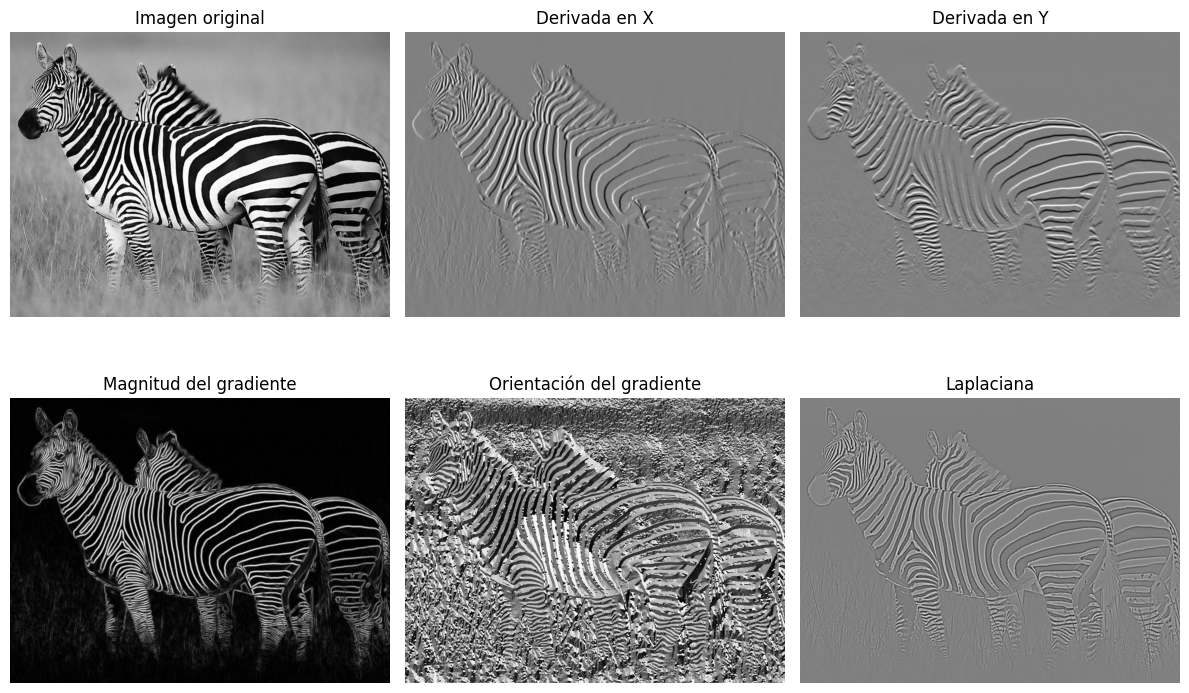
\includegraphics[width=1.0\textwidth, height=0.65\textwidth]{img/sin_titulo2.png}
    \caption{Resultado de la ejecución de la derivada en X, derivada en Y, magnitud del gradiente, orientación del gradiente y el Laplaciano de la imagen original}
    \label{fig:enter-label}
\end{figure}



 \noindent En efecto, atendiendo a dicha figura, comprobamos que:
\begin{itemize}
    \item Cuando derivamos con respecto a \textbf{x}, se realzan los bordes verticales ya que estamos buscando cambios abruptos de intensidad en el eje \textbf{x}. De manera análoga ocurre cuando derivamos con respecto a \textbf{y}, ya que lo que estamos haciendo es medir la tasa de variación de la intensidad en este eje detectando por tanto los bordes horizontales. Los bordes pueden ser blancos o negros, dependiendo de si ha habido un aumento o una disminución de intensidad.
    \item La magnitud del gradiente engloba ambas derivadas, y por eso podemos detectar tanto los bordes verticales como horizontales.
    \item La orientación del gradiente nos muestra información sobre la dirección en la que cambia la intensidad de la imagen.
    \item  El Laplaciano  combina contribuciones de ambas derivadas de segundo orden, lo que facilita la detección de bordes tanto verticales como horizontales. Esto lo convierte en una excelente opción para la detección de características.
\end{itemize}


\section{Núcleos de Sumabilidad}
La proposición \ref{prop:conv} afirma que $\mathscr{L}^1(\mathbb{R}^n)$ tiene estructura de anillo con respecto a las operaciones $+$ y $*$. Sin embargo, debemos notar que $\mathscr{L}^1(\mathbb{R}^n)$ carece de unidad. 

\noindent En efecto, supongamos que exista $K \in \mathscr{L}^1(\mathbb{R}^n)$ tal que se verificara 
\begin{equation}
    K * f = f * K = f \quad \forall f \in \mathscr{L}^1(\mathbb{R}^n).
\end{equation}
Entonces, tomando $f = G \in \mathscr{L}^1(\mathbb{R}^n)$, tenemos
\begin{equation}
   \widehat{K}(y)G(y) =  \widehat{K}(y)\widehat{G}(y) = G(y) \quad \forall y \in \mathbb{R}^n,
\end{equation}
de donde deducimos que necesariamente $\widehat{K}(y) = 1 \, \, \forall y \in \mathbb{R}^n$. Sin embargo, esto contradice el Lema de Riemann-Lebesgue.

\noindent Esta irregularidad no se presenta en el contexto discreto. Estudiaremos este hecho con mayor detenimiento en la segunda parte de la memoria. En ella, analizaremos el filtro impulso, que será aquel que, convolucionándolo con cualquier señal, resulte en ella misma. Vale la pena mencionar, en relación al análisis realizado en el capítulo anterior acerca de las operaciones de correlación y convolución, que este fenómeno no se manifiesta con la operación de correlación, marcando así una clara distinción entre ambas técnicas, y subrayando la convolución como una operación más intuitiva en términos de frecuencia, ya que proporciona una salida más natural.


\noindent No obstante, $\mathscr{L}^1(\mathbb{R}^n)$ cuenta con unidades aproximadas, denominadas núcleos de sumabilidad, que trataran de paliar los indeseados efectos provocados por la ausencia de unidad.

\noindent Previo a establecer de forma adecuadamente amplia el concepto de núcleo de sumabilidad, introducimos algunas definiciones.

\begin{definicion}
   Un \textit{conjunto dirigido} es un conjunto $\Lambda$ provisto de un orden $\leq$, tal que para cualesquiera $\lambda_1,\lambda_2 \in \Lambda$ existe $\mu \in \Lambda$ con $\lambda_1\leq \mu$ y  $\lambda_2\leq \mu$.
\end{definicion}

\begin{definicion}
   Una \textit{red} en un espacio topológico $X$ es una familia $\{x_{\lambda}\}_{\lambda \in \Lambda}$, donde $\Lambda$ es un conjunto dirigido.
\end{definicion}

\noindent Se dice que la red es convergente si existe $x \in X$ tal que para cada entorno $U$ de $x$ existe $\mu \in \Lambda$ tal que 
\begin{equation}
    \mu \in \Lambda, \mu \leq \lambda \implies x_{\lambda} \in U.
\end{equation}
\noindent Si $X$ es un espacio Hausdorff, entonces el punto $x$ es necesariamente único y se denota por $\lim_{\lambda \in \Lambda} \,$.


\begin{ejemplo}
Veamos algunos ejemplos para familiarizarnos con estas definiciones.
\begin{itemize}
    \item Tomamos como conjunto dirigido $\mathbb{N}_0$ con orden creciente, en cuyo caso 
    \begin{equation}
    \lim_{\lambda \in \Lambda} =     \lim_{n \rightarrow \infty}.
    \end{equation}
    \item Tomamos como conjunto dirigido $\mathbb{R}^+$ con orden decreciente, en cuyo caso 
    \begin{equation}
    \lim_{\lambda \in \Lambda} 
 = \lim_{\substack{t \rightarrow 0 \\ t > 0}}.
    \end{equation}
\end{itemize}
    
\end{ejemplo}

\noindent Definimos finalmente el concepto de núcleo de sumabilidad $\{K_{\lambda}\}_{\lambda \in \Lambda}$, que como puede intuir el lector poseerá la cualidad 
\begin{equation}
    \lim_{\lambda \in \Lambda} ||f*K-f||_1=0 \quad  \forall f \in \mathscr{L}^1(\mathbb{R}^n).
\end{equation}

\begin{definicion}\label{defnucl}
    Un\textit{ núcleo de sumabilidad} es una red $\{K_{\lambda}\}_{\lambda \in \Lambda}$ de funciones de $\mathscr{L}^1(\mathbb{R}^n)$ que verifica lo siguiente:
    \begin{itemize}
        \item para cada $\lambda \in \Lambda$,
        \begin{equation}
            \int_{\mathbb{R}^n} K_{\lambda}(x) \, dx = 1;
        \end{equation}

        \item existe una constante $M \in \mathbb{R}^+$ tal que, para cada $\lambda \in \Lambda$,
        \begin{equation}
            \int_{\mathbb{R}^n} |K_{\lambda}(x)| \, dx \leq M;
        \end{equation}
        \item  para cada $\delta \in \mathbb{R}^+$, se tiene que 
        \begin{equation}
            \lim_{\lambda \in \Lambda} \int_{||x|| > \delta} |K_{\lambda}(x)|\, dx = 0.
        \end{equation}
        
    \end{itemize}
\end{definicion}



\noindent A continuación, presentamos un resultado que proporciona una amplia gama de núcleos de sumabilidad.



\begin{proposicion}\label{consnuc}
Sea $K  \in \mathscr{L}^1(\mathbb{R}^n)$ tal que 
\begin{equation}
    \int_{\mathbb{R}^n}K(x) \, dx = 1
\end{equation}
y, para cada $\epsilon \in \mathbb{R}^+$, se define $K_{\epsilon}: \mathbb{R} \rightarrow \mathbb{C}$ por
\begin{equation}
    K_{\epsilon}(x) = \epsilon^{-n}K(\epsilon^{-1}x) \quad \forall x \in \mathbb{R}^n.
\end{equation}
Entonces la familia $\{K_{\epsilon}\}_{\epsilon \in \mathbb{R}^+}$ es un \textit{núcleo de sumabilidad}.
\end{proposicion}

\begin{proof}
Comprobaremos las condiciones que debe verificar un núcleo de sumabilidad. 
\begin{itemize}
    \item Para cada $\epsilon \in \mathbb{R}^+$, se tiene realizando un cambio de variable
    \begin{equation}
        \int_{\mathbb{R}^n}K_{\epsilon}(x) dx = \int_{\mathbb{R}^n} \epsilon^{-n}K(\epsilon^{-1}x) \, dx =  \int_{\mathbb{R}^n}K(x) \, dx = 1.
    \end{equation}
    \item   Para cada $\epsilon \in \mathbb{R}^+$, se tiene 
    \begin{equation}
        \int_{\mathbb{R}^n}|K_{\epsilon}(x)| dx = \int_{\mathbb{R}^n} \epsilon^{-n}|K(\epsilon^{-1}x)| \, dx =  \int_{\mathbb{R}^n}|K(x)| \, dx = ||K||_1.
    \end{equation}
    Por tanto, se verifica la segunda condición de la definición \ref{defnucl} con constante $M=||K||_1$.

    \item Fijamos un $\delta \in \mathbb{R}^+$, tenemos por tanto que
    \begin{equation}
        \int_{||x||>\delta} |K_{\epsilon}(x)| \, dx = \int_{||x||>\delta} \epsilon^{-n}|K(\epsilon^{-1}x)| \, dx = \int_{||x||>\delta/\epsilon} |K(x)| \, dx.
    \end{equation}
    Debemos entonces probar que 
    \begin{equation}
    \lim_{\substack{\epsilon \rightarrow 0 \\ \epsilon > 0}}\int_{||x||>\delta/\epsilon} |K(x)| \, dx  = 0.
    \end{equation}
    Para ello, vamos a usar el Teorema de la convergencia dominada.
    Sea $\{\epsilon_m\}$ una sucesión en $\mathbb{R}^+$ tal que $\{\epsilon_m\} \rightarrow 0$. Definimos una sucesión de funciones $\{\phi_m\} \in \mathscr{L}^1(\mathbb{R}^n)$ por
    \begin{equation}
        \phi_m(x) = 
    \begin{cases}
    |K(x)| & \text{si } ||x|| > \delta/\epsilon_m, \\
    0 & \text{si } ||x|| < \delta/\epsilon_m.
    \end{cases}
    \end{equation}
    Observamos que 
    \begin{equation}
        \int_{||x||> \delta/\epsilon_m} |K(x)|\, dx = \int_{\mathbb{R}^n} \phi_m(x) \, dx \quad \forall m \in \mathbb{N}.
    \end{equation}
    Aplicamos entonces el Teorema de la convergencia dominada a $\phi_m$.
    \begin{itemize}
        \item Como  $\{\delta/\epsilon_m\} \rightarrow 0$,
        \begin{equation}
            \lim_{m \rightarrow \infty} \phi_m(x) = 0 \quad \forall x \in \mathbb{R}^n.
        \end{equation}
        \item Se tiene que
        \begin{equation}
            |\phi_m(x)| \leq |K(x)| \quad \forall x \in \mathbb{R}^n, \forall m \in \mathbb{N},
        \end{equation}
        con $|K|$ integrable en $\mathbb{R}^n$.
    \end{itemize}
    Luego el Teorema de la convergencia dominada garantiza que 
    \begin{equation}
        \lim_{m \rightarrow \infty} \int_{\mathbb{R}^n} \phi_m(x) \, dx =0.
    \end{equation}
    De aquí deducimos que
     \begin{equation}
    \lim_{m \rightarrow \infty }\int_{||x||>\delta/\epsilon_m} |K(x)| \, dx  = 0,
    \end{equation}
    cumpliéndose así la última condición.
    
\end{itemize}
Concluimos que para cada $ \epsilon \in \mathbb{R}^+$ la familia $\{K_{\epsilon}\}_{\epsilon \in \mathbb{R}^+}$ es un núcleo de sumabilidad.
\end{proof}



\begin{ejemplo}[Núcleo de Gauss-Weierstrass]
    La familia de funciones $\{G_t\}_{t\downarrow
0}$ definida por
    \begin{equation}
        G_{t}: \mathbb{R}^n \rightarrow \mathbb{R}, \, G_{t}(x) = \frac{1}{(4 \pi t)^{-n/2}}e^{- \pi ||x||^2} \quad \forall x \in \mathbb{R}^n, \forall t \in \mathbb{R}^+,
    \end{equation}
    se denomina \textit{núcleo de Gauss-Weierstrass}.
    
    \vspace{0.1cm}
    \noindent Observamos que este núcleo es la familia de funciones $\{K_{\sqrt{4\pi t}}\}_{t \in \mathbb{R}^+}$ asociada a la proposición \ref{consnuc}, con $K = G \in \mathscr{L}^1(\mathbb{R}^n)$.
\end{ejemplo}

\begin{definicion}\label{gauss}
    Definimos $P : \mathbb{R}^n \rightarrow \mathbb{R}$ función de $  \mathscr{L}^1(\mathbb{R}^n)$ dada por
    \begin{equation}
        P(x) =  C_n \frac{1}{(1 + ||x||^2)^{\frac{n+1}{2}}}, \; \; \; \text{con} \, \, C_n = \frac{\Gamma({\frac{n+1}{2}})}{\pi^{\frac{n+1}{2}}}
    \end{equation}
    y donde $\Gamma$ es la función gamma.
\end{definicion}

\begin{lema}\label{lem:leam}
$P$ cumple
\begin{equation}\label{loq}
    \int_{\mathbb{R}^n} P(x)\, \, dx = 1 .
\end{equation}
\end{lema}
\begin{proof}

Comprobaremos que se verifica
\begin{equation}
        \frac{1}{C_n} = \int_{\mathbb{R}^n} \frac{1}{(1 + ||x||^2)^{\frac{n+1}{2}}} \,dx,
\end{equation}
que es equivalente a~\eqref{loq}.

\noindent Usamos coordenadas polares:
\[
\int_{\mathbb{R}^n} \frac{1}{(1 + ||x||^2)^{\frac{n+1}{2}}} \, dx \,  = w_{n-1}\int_{0}^{\infty} \frac{r^{n-1}}{(1+r^2)^{\frac{n+1}{2}}} dr,
\]
donde $w_{n-1}$ denota el área de $\mathbb{S}^{n-1}$.

\noindent Aplicamos el cambio de variable, \(r = \tan(\theta)\), y obtenemos
\begin{align}
 w_{n-1}\int_{0}^{\infty} \frac{r^{n-1}}{(1+r^2)^{\frac{n+1}{2}}} dr &=  w_{n-1}\int_{0}^{\pi/2} \frac{(\tan(\theta))^{n-1}}{(1+(\tan(\theta))^2)^{\frac{n+1}{2}}} (1+ \tan(\theta))^2 d\theta \\
 &=  w_{n-1}\int_{0}^{\pi/2} \frac{(\tan(\theta))^{n-1}(\cos(\theta))^{n+1}}{(\cos(\theta))^2} d\theta \\
 &=  w_{n-1}\int_{0}^{\frac{\pi}{2}} (\sin(\theta))^{n-1} d\theta.
\end{align}

\noindent Realizando el cambio de variable $u = (\sin(\theta))^2$, resulta
\[
w_{n-1}\int_{0}^{\frac{\pi}{2}} (\sin(\theta))^{n-1} d\theta =  \frac{1}{2}w_{n-1}\int_{0}^{1} (1-s)^{\frac{n}{2}-1}s^{\frac{1}{2}-1} ds = \frac{1}{2}w_{n-1}\beta\left(\frac{n}{2},\frac{1}{2}\right).
\]
Sustituyendo ahora el valor de $w_{n-1}$ y utilizando la relación de la función beta $\beta$ con la función gamma $\Gamma$, se tiene:
\[
 w_{n-1}\beta\left(\frac{n}{2},\frac{1}{2}\right)= \frac{2 \Gamma\left(\frac{n}{2}\right) \Gamma\left(\frac{1}{2}\right)}{\Gamma\left(\frac{n+1}{2}\right)} = \frac{\pi^{\frac{n+1}{2}}}{\Gamma\left(\frac{n+1}{2}\right)}.
\]
Concluimos que
\begin{equation*}
\int_{\mathbb{R}^n} \frac{1}{(1 + ||x||^2)^{\frac{n+1}{2}}} \, dx =
\frac{\pi^{\frac{n+1}{2}}}{\Gamma\left(\frac{n+1}{2}\right)} = \frac{1}{C_n}.  \qedhere
\end{equation*}
 
\end{proof}


\begin{ejemplo}[Núcleo de Poisson]
    La familia de funciones $\{P_y\}_{y\downarrow
0}$ definida por
    \begin{equation}
        P_{y}: \mathbb{R}^n \rightarrow \mathbb{R}, \; \; \; \, P_{y}(x) = C_n \frac{y}{(y^2 + ||x||^2)^{\frac{n+1}{2}}}, \; \; \; \; \text{con} \, \, C_n = \frac{\Gamma({\frac{n+1}{2}})}{\pi^{\frac{n+1}{2}}},
    \end{equation}
    se denomina \textit{núcleo de Poisson}.

    \noindent Observamos que este núcleo es la familia de funciones $\{K_{y}\}_{y \in \mathbb{R}^+}$ asociada a la proposición \ref{consnuc} con $K = P \in \mathscr{L}^1(\mathbb{R}^n)$.
\end{ejemplo}

\begin{lema}\label{lema:previo}
    Sea $K  \in \mathscr{L}^1(\mathbb{R}^n)$ tal que 
\begin{equation}
    \int_{\mathbb{R}^n}K(x) \, dx = 1.
\end{equation}
Supongamos $1 \leq p < \infty$, y $f \in \mathscr{L}^p(\mathbb{R}^n)$. Entonces
\begin{equation}
|| f*K_{\lambda}-f||_p \leq \int_{\mathbb{R}^n} w_pf(x) |K_{\lambda}(x)| \, dx.
\end{equation}
\end{lema}
\begin{proof}
\noindent Para cada  $x \in \mathbb{R}^n$ tal que $(f*K)(x)$ está definida, tenemos 
 \begin{align}
    |(f*K)(x)-f(x)| &= \left|\int_{\mathbb{R}^n}f(x-t)K(t) \, dt - f(x) \int_{\mathbb{R}^n}K(t) \,dt \right| \\
    &\leq \int_{\mathbb{R}^n} \left|f(x-t)-f(x) \right| |K(t)| \, dt. \\ 
\end{align}
\noindent Distinguimos dos casos:
\begin{itemize}
    \item Suponemos que $p=1$. Usando el Teorema de Tonelli, tenemos que
    \begin{align*}
        ||f*K-f||_1 &= \int_{\mathbb{R}^n} |(f*K_{\lambda})(x)-f(x)| \, dx\\
        &\leq \int_{\mathbb{R}^n} \int_{\mathbb{R}^n} \left|f(x-t)-f(x) \right| |K_{\lambda}(t)| \, dt \, dx \\
        &= \int_{\mathbb{R}^n} \int_{\mathbb{R}^n} \left|f(x-t)-f(x) \right| |K(t)| \, dx \, dt  =\int_{\mathbb{R}^n} w_1f(t) |K(t)|\, dt.
    \end{align*}
    \item Suponemos que $1<p<\infty$. Tomamos $q = \frac{p}{p-1}$, de modo que $\frac{1}{p}+\frac{1}{q}=1$.
    Aplicando el Teorema de Tonelli de nuevo, obtenemos
    \begin{align}
    ||f*K-f||_p^p &= \int_{\mathbb{R}^n}|(f*K_{\lambda})(x)-f(x)|^p \, dx  =  \\
    &\leq \int_{\mathbb{R}^n} |(f*K_{\lambda})(x)-f(x)||(f*K_{\lambda})(x)-f(x)|^{p-1} \, dx. \\ 
    &\leq \int_{\mathbb{R}^n} \left(\int_{\mathbb{R}^n} \left|f(x-t)-f(x) \right| |K(t)| \, dt \right)|(f*K_{\lambda})(x)-f(x)|^{p-1} \, dx. \\ 
    &\leq \int_{\mathbb{R}^n} \left(\int_{\mathbb{R}^n} \left|f(x-t)-f(x) \right| |(f*K_{\lambda})(x)-f(x)|^{p-1} \,dx \right) |K(t)|\, dt. \\ 
\end{align}
    Ahora aplicamos la desigualdad de H\"{o}lder 
    \begin{align}
    &\int_{\mathbb{R}^n} \left(\int_{\mathbb{R}^n} \left|f(x-t)-f(x) \right| |(f*K_{\lambda})(x)-f(x)|^{p-1} \,dx \right) \\
    &\leq \left( \int_{\mathbb{R}^n} \left|f(x-t)-f(x) \right|^p \, dx  \right)^{1/p} \left( \int_{\mathbb{R}^n} |(f*K_{\lambda})(x)-f(x)|^{(p-1)q} \, dx  \right)^{1/q} \\
    &\leq \left( \int_{\mathbb{R}^n} \left|f(x-t)-f(x) \right|^p \, dx  \right)^{1/p} \left( \int_{\mathbb{R}^n} |(f*K_{\lambda})(x)-f(x)|^{p} \, dx  \right)^{1/q}  \\
    &= w_pf(t)||f*K-f||_p^{p/q}.
\end{align}
\noindent De donde deducimos que 
\begin{equation}
       ||f*K-f||_p^p \leq \int_{\mathbb{R}^n} w_pf(t)||f*K-f||_p^{p/q} |K(t)|\, dt = ||f*K-f||_p^{p/q}\int_{\mathbb{R}^n} w_pf(t) |K(t)|\, dt,
\end{equation}
\noindent luego 
\begin{equation}
       ||f*K-f||_p \leq \int_{\mathbb{R}^n} w_pf(t) |K(t)|\, dt.
\end{equation}
\end{itemize}
En ambos casos se verifica la desigualdad. 
\end{proof}






\begin{teorema} \label{teo:suma}
    Sea $\{K_{\lambda}\}_{\lambda \in \Lambda}$ un núcleo de sumabilidad. Supongamos $1 \leq p < \infty$, y $f \in \mathscr{L}^p(\mathbb{R}^n)$. Entonces
    \begin{equation}
        \lim_{\lambda \in \Lambda} ||f*K_{\lambda}-f||_p=0.
    \end{equation}
\end{teorema}
\begin{proof}
Fijamos $\delta \in \mathbb{R}^+$, para cada $\lambda \in \Lambda$, usando el Lema \ref{lema:previo}, se tiene que
\begin{align}
    || f*K_{\lambda}-f||_p &\leq \int_{\mathbb{R}^n} w_pf(x) |K_{\lambda}(x)| \, dx \\
    &= \int_{||x|| < \delta} w_pf(x) |K_{\lambda}(x)| \, dx +\int_{||x|| > \delta} w_pf(x) |K_{\lambda}(x)| \, dx.
\end{align}
\noindent Analizamos cada uno de los sumandos por separado. Para el primero, usamos que $K_{\lambda}$ es un núcleo de sumabilidad:
\begin{equation}
    \int_{||x|| < \delta} w_pf(x) |K_{\lambda}(x)| \, dx \leq \sup_{||x|| < \delta}w_pf(x)\int_{||x|| < \delta} |K_{\lambda}(x)| \, dx  \leq M\sup_{||x|| < \delta}w_pf(x).
\end{equation}
\noindent Y, por otro, usando la proposición \ref{mod_cont}, sabemos que
\begin{equation}
    \int_{||x|| > \delta} w_pf(x) |K_{\lambda}(x)| \, dx \leq 2 ||f||_p\int_{||x|| > \delta} |K_{\lambda}(x)| \, dx.
\end{equation}

\noindent Juntando ambas acotaciones,   
\begin{equation}
     || f*K_{\lambda}-f||_p \leq M\sup_{||x|| < \delta}w_pf(x)+ 2 ||f||_p\int_{||x|| > \delta} |K_{\lambda}(x)| \, dx.
\end{equation}
Luego
\begin{equation}
    \limsup_{\lambda \in \Lambda}|| f*K_{\lambda}-f||_p \leq M\sup_{||x|| < \delta}w_pf(x).
\end{equation}
Esto es válido para todo $\delta \in \mathbb{R}^+$, por lo que 
\begin{equation}
    \lim_{\delta \rightarrow 0}\sup_{||x|| < \delta}w_pf(x)= 0.
\end{equation}
En consecuencia
\begin{equation}
    \limsup_{\lambda \in \Lambda}|| f*K_{\lambda}-f||_p =0,
\end{equation}
concluyendo que 
\begin{equation*}
    \lim_{\lambda \in \Lambda}|| f*K_{\lambda}-f||_p =0.\qedhere
\end{equation*}
\end{proof}


\begin{corolario} \label{coro:coro}
    Sea $K  \in \mathscr{L}^1(\mathbb{R}^n)$ tal que 
    \begin{equation}
        \int_{\mathbb{R}^n}K(x) \, dx = 1.
    \end{equation}
    Para cada $\epsilon \in \mathbb{R}^+$, se define $K_{\epsilon}: \mathbb{R} \rightarrow \mathbb{C}$ por
    \begin{equation}
        K_{\epsilon}(x) = \epsilon^{-n}K(\epsilon^{-1}x) \quad \forall x \in \mathbb{R}^n.
    \end{equation}
     Supongamos $1 \leq p < \infty$, y $f \in \mathscr{L}^p(\mathbb{R}^n)$. Entonces
    \begin{equation}
        \lim_{\substack{\epsilon \rightarrow 0 \\ \epsilon > 0}} ||f* K_{\epsilon}-f||_p=0.
    \end{equation}
\end{corolario}


\begin{proof}
    Basta con usar el Teorema \ref{teo:suma}, y la Proposición \ref{consnuc}.
\end{proof}




\begin{teorema} \label{contnuc}
    Sea $\{K_{\lambda}\}_{\lambda \in \Lambda}$ un núcleo de sumabilidad, y $f \in \mathscr{L}^{\infty}(\mathbb{R}^n)$.
    \begin{itemize}
        \item Supongamos que $f$ es continua en cada punto de un subconjunto compacto $E \subset \mathbb{R}^n$. Entonces
        \begin{equation}
            \lim_{\lambda  \in \Lambda} \max_{x \in E} |(f*K_{\lambda})(x)-f(x)|=0.
        \end{equation}
        En particular, si $f$ es continua en un punto $x \in \mathbb{R}^n$,
         \begin{equation}\label{punt}
            \lim_{\lambda  \in \Lambda} (f*K_{\lambda})(x)=f(x).
        \end{equation}
        \item Supongamos que $f$ es uniformemente continua en $\mathbb{R}^n$. Entonces
        \begin{equation}
            \lim_{\lambda  \in \Lambda} ||(f*K_{\lambda})(x)-f(x)||_{\infty}=0.
        \end{equation}
    \end{itemize}
\end{teorema}
\begin{proof}
    Como $f \in \mathscr{L}^{\infty}(\mathbb{R}^n)$, sabemos que la convolución $f*K_\lambda$ está definida en todo $\mathbb{R}^n$ y está acotada. Dado $\epsilon \in \mathbb{R}^+$, notemos los siguientes puntos: 
    \begin{itemize}
    
        \item Por la continuidad de $f$ en cada punto del conjunto compacto $E$, se tiene que $\exists \delta \in \mathbb{R}^+$ tal que 
        \begin{equation}
            x \in E, \, ||x-t||< \delta \implies |f(x-t)-f(x)| < \frac{\epsilon}{2M}.
        \end{equation}
        
        \item Al ser $\{K_{\lambda}\}_{\lambda \in \Lambda}$ un núcleo de sumabilidad, existe $ M >0$ tal que para todo $ \lambda \in \Lambda$
        \begin{equation}
             \int_{\mathbb{R}^n} |{K_\lambda}(x)| \, dx \leq M.
        \end{equation}
        Además, también existe $ \mu \in \Lambda$ tal que
        \begin{equation}
            \lambda \in \Lambda, \mu \leq \lambda \implies 2 ||f||_\infty   \int_{||x|| > \delta} |K_{\lambda}(x)|\, dx < \frac{\epsilon}{2}.
        \end{equation} 
    \end{itemize}

    \noindent Para $\lambda \in \Lambda$ con $ \mu \leq \lambda$, y para cada $x \in E$, usando los puntos anteriores, se tiene que
    
     \begin{align*}
        |(f*K_{\lambda})(x)-f(x)| &= \left|\int_{\mathbb{R}^n}f(x-t)K_{\lambda}(t) \, dt - f(x) \int_{\mathbb{R}^n}K_{\lambda}(t) \,dt \right| \\
        &\leq \int_{\mathbb{R}^n} \left|f(x-t)-f(x) \right| |K_{\lambda}(t)| \, dt \\
        &=   \int_{||t|| < \delta} \left|f(x-t)-f(x) \right| |K_{\lambda}(t)| \, dt + \int_{||t|| > \delta} \left|f(x-t)-f(x) \right| |K_{\lambda}(t)| \, dt \\ 
        &\leq \frac{\epsilon}{2M}\int_{||t|| < \delta}  |K_{\lambda}(t)| \, dt + 2 ||f||_\infty\int_{||t|| > \delta} |K_{\lambda}(t)| \, dt 
        \leq \frac{\epsilon}{2M}M + \frac{\epsilon}{2} = \epsilon.
    \end{align*}


    \noindent Por tanto,
    
    \begin{equation}
        \max_{x \in E} |(f*K_{\lambda})(x)-f(x)| \leq \epsilon.
    \end{equation}
    Finalmente, si $f$ es continua en un punto $x \in \mathbb{R}^n$, tomando como conjunto compacto $E = \{x\}$, se sigue que 
    \begin{equation*}\label{punt}
            \lim_{\lambda  \in \Lambda} (f*K_{\lambda})(x)=f(x).\qedhere
        \end{equation*}
\end{proof}


\begin{corolario}  \label{coro2}
    Sea $K  \in \mathscr{L}^1(\mathbb{R}^n)$ tal que 
    \begin{equation}
        \int_{\mathbb{R}^n}K(x) \, dx = 1.
    \end{equation}
    Para cada $\epsilon \in \mathbb{R}^+$, se define $K_{\epsilon}: \mathbb{R} \rightarrow \mathbb{C}$ por
    \begin{equation}
        K_{\epsilon}(x) = \epsilon^{-n}K(\epsilon^{-1}x) \quad \forall x \in \mathbb{R}^n.
    \end{equation}
     Sea también $f \in \mathscr{L}^{\infty}(\mathbb{R}^n)$.
    \begin{itemize}
        \item Supongamos que $f$ es continua en cada punto de un subconjunto compacto $E \subset \mathbb{R}^n$. Entonces
        \begin{equation}
            \lim_{\substack{\epsilon \rightarrow 0 \\ \epsilon > 0}} \max_{x \in E} |(f*K_{\epsilon})(x)-f(x)|=0.
        \end{equation}
        En particular, si $f$ es continua en un punto $x \in \mathbb{R}^n$,
         \begin{equation}
            \lim_{\substack{\epsilon \rightarrow 0 \\ \epsilon > 0}} (f*K_{\epsilon})(x)=f(x).
        \end{equation}
        \item Supongamos que $f$ es uniformemente continua en $\mathbb{R}^n$. Entonces
        \begin{equation}
           \lim_{\substack{\epsilon \rightarrow 0 \\ \epsilon > 0}} ||(f*K_{\epsilon})(x)-f(x)||_{\infty}=0.
        \end{equation}
    \end{itemize}
\end{corolario}


\begin{proof}
    Basta con usar el Teorema \ref{contnuc}, y la proposición \ref{consnuc}.
\end{proof}

\begin{observacion}
    Cabe mencionar que en el segundo apartado del Teorema \ref{contnuc} y el Corolario \ref{coro2} se exige que la función $f$ sea uniformemente continua, y esta condición no es caprichosa. En efecto, como hemos anotado anteriormente, al estar $f \in \mathscr{L}^{\infty}(\mathbb{R}^n)$, se tiene que  para todo $\lambda \in \Lambda, \, \,\,  f*K_{\lambda}$ es uniformemente continua en $\mathbb{R}^n$, por lo que si se cumple que
    \begin{equation}
            \lim_{\lambda  \in \Lambda} ||(f*K_{\lambda})(x)-f(x)||_{\infty}=0,
    \end{equation}
    se tiene que necesariamente $f$ es uniformemente continua en $\mathbb{R}^n$.
\end{observacion}


\noindent

\section{Métodos de Sumación}

Retomamos en esta sección el desafío de reconstruir una función $f \in \mathscr{L}^1(\mathbb{R}^n)$ a partir de su Transformada de Fourier $\widehat{f}$. El lector puede pensar que este objetivo ya se alcanzó mediante  el Teorema de Inversión. Sin embargo, para su aplicación, se  obligaba a que necesariamente la función Transformada fuera integrable en $\mathbb{R}^n$ (de hecho, si no lo era, no tenía sentido la reconstrucción planteada en~\eqref{eq:teoinv}). Sin embargo, como ya comentamos en el primer capítulo, esta es una hipótesis ciertamente restrictiva, y es por ello por lo que se plantean otras posibles interpretaciones para reconstruir la función.

\vspace{0.5cm}
\noindent Recordamos los métodos se sumabilidad de las series de Fourier, que consistían en la utilización de las sumas ponderadas 
\begin{equation}
    \sum_{k=-\infty}^{\infty}\widehat{f}(k)e^{ikx}\Phi(\epsilon k),
\end{equation}
donde $\Phi$ era una función de peso adecuada y la ejecución del límite en $\epsilon = 0$ de éstas.
Parece natural tratar de utilizar en nuestra situación integrales ponderadas
\begin{equation}
 \int_{\mathbb{R}^n}\widehat{f}(y)e^{2\pi i \langle x, y \rangle} \Phi(\epsilon y) \, dy 
\end{equation}
y ejecutar el límite en $\epsilon = 0$. 

\begin{proposicion} \label{ame}
    Sea $\Phi \in \mathscr{L}^1(\mathbb{R}^n)$ tal que
    \begin{equation}
        \Phi(-x) = \Phi(x) \quad \forall x \in \mathbb{R}^n,
    \end{equation}
y pongamos $K = \widehat{\Phi}$. Para cada $ \epsilon \in \mathbb{R}^+$, se define la función $K_{\epsilon}: \mathbb{R} \rightarrow \mathbb{C}$ por
\begin{equation}
    K_{\epsilon}(x) = \epsilon^{-n}K(\epsilon^{-1}x) \quad \forall x \in \mathbb{R}^n.
\end{equation}
Supongamos $f \in \mathscr{L}^1(\mathbb{R}^n)$. Entonces se verifica
\begin{equation}\label{eq:c }
     \int_{\mathbb{R}^n}\widehat{f}(y)e^{2\pi i \langle x, y \rangle} \Phi(\epsilon y) \, dy  = (f*K_{\epsilon})(x) \quad \forall x \in \mathbb{R}^n, \forall \epsilon \in \mathbb{R}^+.
\end{equation}
\end{proposicion}

\begin{proof}
   \noindent Comenzamos anotando los siguientes hechos: 
   \begin{itemize}
       \item Por un lado, sabemos que la función $y \mapsto \widehat{f}(y)e^{2\pi i \langle x, y \rangle} \Phi(\epsilon y)$ es el producto de una función continua y acotada $y \mapsto \widehat{f}(y)e^{2\pi i \langle x, y \rangle}$ por una función integrable   $y  \mapsto \Phi(\epsilon y)$.
       \item Como $K$ es la Transformada de Fourier de una función integrable en $\mathbb{R}^n$, sabemos que está acotada en $\mathbb{R}^n$. Luego también lo está $K_{\epsilon}$, y eso hace que la convolución $f*K_{\epsilon}$ esté definida en todo $\mathbb{R}^n$.
       \item Como $\Phi(x) = \Phi(-x) \quad \forall x \in \mathbb{R}^n$, se sigue que $K(x) = K(-x)$, y entonces $K_{\epsilon}(x) = K_{\epsilon}(-x) \quad \forall x \in \mathbb{R}^n, \, \forall \epsilon \in \mathbb{R}^+.$
   \end{itemize}
   \item Fijamos $x \in \mathbb{R}^n$ y $\epsilon \in \mathbb{R}^+$. Se tiene que
  \begin{equation*}
    \begin{aligned}
      \int_{\mathbb{R}^n} \widehat{f}(y)e^{2 \pi i \langle x,y \rangle}\Phi(\epsilon y) \, dy
        &= \int_{\mathbb{R}^n} \widehat{\tau_{-x}f}(y)H_{\epsilon}\Phi(y) \, dy 
        = \int_{\mathbb{R}^n} \tau_{-x}f(y) \widehat{H_{\epsilon}\Phi}(y) \, dy \\
        &= \int_{\mathbb{R}^n} \tau_{-x}f(y)\epsilon^{-n}\widehat{\Phi}(\epsilon^{-1}y) \, dy 
        = \int_{\mathbb{R}^n} \tau_{-x}f(y)K_{\epsilon}(y) \, dy \\
        &= \int_{\mathbb{R}^n} f(x+y)K_{\epsilon}(y) \, dy 
        = \int_{\mathbb{R}^n} f(x-y)K_{\epsilon}(-y) \, dy \\
        &= \int_{\mathbb{R}^n} f(x-y)K_{\epsilon}(y) \, dy 
        = (f * K_{\epsilon})(x).
    \end{aligned}
\end{equation*}
Por tanto, hemos probado~\eqref{eq:c}.
\end{proof}


\begin{lema}\label{lema}
Sea $\Phi \in \mathscr{L}^1{(\mathbb{R}^n)}$ y supongamos que se cumplen las siguientes condiciones:
\begin{itemize}
    \item $\Phi$ es continua en $0$, 
    \item $\Phi(0) = 1$,
    \item $\widehat{\Phi} \in \mathscr{L}^1(\mathbb{R}^n).$
\end{itemize}
Entonces, 
\begin{equation}
    \int_{\mathbb{R}^n} \widehat{\Phi}(y) \, dy = 1.
\end{equation}
\end{lema}

\begin{proof}
    Basta con aplicar el Teorema de Inversión a $\Phi$, cuya Transformada es integrable en $\mathbb{R}^n$. Como $\Phi $ es continua en $0$, se tiene que 
    \begin{equation}
        1 = \Phi(0) = \int_{\mathbb{R}^n} \widehat{\Phi}(y) \, dy.
    \end{equation}
\end{proof}

\begin{teorema}\label{teoteo}
    Sea $\Phi \in \mathbb{R}^n$ y suponemos que se verifica que
    \begin{itemize}
         \item $\Phi$ es continua en $0$, 
    \item $\Phi(0) = 1$,
    \item $\widehat{\Phi} \in \mathscr{L}^1(\mathbb{R}^n).$
    \end{itemize}
    Si $f \in \mathscr{L}^1(\mathbb{R}^n)$, entonces
    \begin{equation}
        \lim_{\substack{\epsilon \rightarrow 0 \\ \epsilon > 0}} \int_{\mathbb{R}^n} \left| f(x) -   \int_{\mathbb{R}^n}\widehat{f}(y)e^{2\pi i \langle x, y \rangle} \Phi(\epsilon y) \, dy \right| \, dx = 0.
    \end{equation}
\end{teorema}
\begin{proof}
Sea $K = \widehat{\Phi}$. Por un lado, sabemos por la proposición \ref{ame}  que 
\begin{equation}\label{eq:c }
     \int_{\mathbb{R}^n}\widehat{f}(y)e^{2\pi i \langle x, y \rangle} \Phi(\epsilon y) \, dy  = (f*K_{\epsilon})(x) \quad \forall x \in \mathbb{R}^n, \forall \epsilon \in \mathbb{R}^+.
\end{equation}
\noindent Por otra parte, sabemos que por el Lema \ref{lema} se cumple que 
\begin{equation}
    \int_{\mathbb{R}^n} K(x) \, dx = 1.
\end{equation}
\noindent Por tanto, aplicando el Corolario \ref{coro:coro} se tiene que 
\begin{equation*}
    0 = \lim_{\substack{\epsilon \rightarrow 0 \\ \epsilon > 0}}||f-f*K_{\epsilon}||_1  = \lim_{\substack{\epsilon \rightarrow 0 \\ \epsilon > 0}} \int_{\mathbb{R}^n} \left| f(x) -   \int_{\mathbb{R}^n}\widehat{f}(y)e^{2\pi i \langle x, y \rangle} \Phi(\epsilon y) \, dy \right| \, dx = 0. \qedhere
\end{equation*}
\end{proof}
\begin{teorema}\label{teoteoteo}
    Sea $\Phi \in \mathbb{R}^n$ y suponemos que se verifica que
    \begin{itemize}
         \item $\Phi$ es continua en $0$, 
    \item $\Phi(0) = 1$,
    \item $\widehat{\Phi} \in \mathscr{L}^{\infty}(\mathbb{R}^n).$
    \end{itemize}
    Si $f \in \mathscr{L}^{\infty}(\mathbb{R}^n)$, entonces
    \begin{itemize}
        \item Supongamos que $f$ es continua en cada punto de un subconjunto compacto $E \subset \mathbb{R}^n$. Entonces
        \begin{equation}
             \lim_{\substack{\epsilon \rightarrow 0 \\ \epsilon >0}}\int_{\mathbb{R}^n}\widehat{f}(y)e^{2\pi i \langle x, y \rangle} \Phi(\epsilon y) \, dy  = f(x)
        \end{equation}
        uniformemente en $E$, esto es, 
         \begin{equation}
        \lim_{\substack{\epsilon \rightarrow 0 \\ \epsilon > 0}} \max_{x \in E}  \left| f(x) -   \int_{\mathbb{R}^n}\widehat{f}(y)e^{2\pi i \langle x, y \rangle} \Phi(\epsilon y) \, dy \right|  = 0.
    \end{equation}
    En particular, si $f$ es continua en un punto $x \in \mathbb{R}^n$, entonces
    \begin{equation}
             \lim_{\substack{\epsilon \rightarrow 0 \\ \epsilon > 0}}\int_{\mathbb{R}^n}\widehat{f}(y)e^{2\pi i \langle x, y \rangle} \Phi(\epsilon y) \, dy  = f(x). 
        \end{equation}

    \item  Si $f$ es uniformemente continua en $\mathbb{R}^n$, entonces
    \begin{equation}
              \lim_{\substack{\epsilon \rightarrow 0 \\ \epsilon >0}}\int_{\mathbb{R}^n}\widehat{f}(y)e^{2\pi i \langle x, y \rangle} \Phi(\epsilon y) \, dy  = f(x)
        \end{equation}
        uniformemente en $\mathbb{R}^n$,
        esto es, 
         \begin{equation}
        \lim_{\substack{\epsilon \rightarrow 0 \\ \epsilon > 0}} \sup_{x \in \mathbb{R}^n}  \left| f(x) -   \int_{\mathbb{R}^n}\widehat{f}(y)e^{2\pi i \langle x, y \rangle} \Phi(\epsilon y) \, dy \right|   = 0.
    \end{equation}
    \end{itemize}
\end{teorema}
\begin{proof}
Sea $K = \widehat{\Phi}$. Por un lado sabemos por la proposición \ref{ame}  que 
\begin{equation}\label{eq:c }
     \int_{\mathbb{R}^n}\widehat{f}(y)e^{2\pi i \langle x, y \rangle} \Phi(\epsilon y) \, dy  = (f*K_{\epsilon})(x) \quad \forall x \in \mathbb{R}^n, \forall \epsilon \in \mathbb{R}^+.
\end{equation}
\noindent Por otra parte, sabemos que por el Lema \ref{lema} se cumple que 
\begin{equation}
    \int_{\mathbb{R}^n} K(x) \, dx = 1.
\end{equation}
Además,
\begin{equation}
    |K(x)| = |\widehat{\Phi}(x)| \leq ||\Phi||_1 \quad \forall x \in \mathbb{R}^n.
\end{equation}
\noindent El Corolario \ref{contnuc} proporciona el resultado deseado.
\end{proof}
\begin{observacion}
   Es posible prescindir de la condición de $ f \in \mathscr{L}^{\infty}(\mathbb{R}^n)$ con una teoría más extensa sobre los núcleos de sumabilidad. Este aspecto se reserva para trabajo futuro.
\end{observacion}

\subsection{Método de Sumación de Gauss}

Sea $f \in \mathscr{L}^1(\mathbb{R}^n).$ El\textit{ método de sumación de Gauss} consiste en utilizar el límite
\begin{equation}
     \lim_{\substack{\epsilon \rightarrow 0 \\ \epsilon > 0}} \int_{\mathbb{R}^n}\widehat{f}(y)e^{2\pi i \langle x, y \rangle} e^{-\epsilon ||y|| ^2} \, dy
\end{equation}
como mecanismo de inversión de la Transformada de Fourier de $f$.

\noindent Para cada $\epsilon \in \mathbb{R}^+$ y cada  $x \in \mathbb{R}^n$, se tiene que
\begin{equation}
    \int_{\mathbb{R}^n}\widehat{f}(y)e^{2\pi i \langle x, y \rangle} e^{-\epsilon ||y|| ^2} \, dy = \int_{\mathbb{R}^n}\widehat{f}(y)e^{2\pi i \langle x, y \rangle} G\left(\frac{\sqrt{\epsilon}}{\sqrt{\pi}}y\right) \, dy. 
\end{equation}

\noindent Sabemos que 
\begin{itemize}
    \item $G \in \mathscr{L}^1(\mathbb{R}^n)$,
    \item $G$ es continua en $\mathbb{R}^n$,
    \item $G(0)=1$,
    \item $G(x)=G(-x)$,
    \item $\widehat{G}=G \in \mathscr{L}^1(\mathbb{R}^n)$.
\end{itemize}

\begin{corolario}
    Si $f \in \mathscr{L}^1(\mathbb{R}^n)$, entonces
    \begin{equation}
        \lim_{\substack{\epsilon \rightarrow 0 \\ \epsilon > 0}} \int_{\mathbb{R}^n} \left| f(x) -   \int_{\mathbb{R}^n}\widehat{f}(y)e^{2\pi i \langle x, y \rangle} e^{-\epsilon ||y||^2} \, dy \right| \, dx = 0.
    \end{equation}
\end{corolario}
\begin{proof}
    El resultado se deduce del Teorema \ref{teoteo}, tomando $\Phi = G$ y como $\epsilon$ tomamos $\frac{\sqrt{\epsilon}}{\sqrt{\pi}}$.
\end{proof}


\begin{teorema}

    Sea $f \in \mathscr{L}^{\infty}(\mathbb{R}^n)$.
    \begin{itemize}
        \item Supongamos que $f$ es continua en cada punto de un subconjunto compacto $E \subset \mathbb{R}^n$. Entonces
        \begin{equation}
             \lim_{\substack{\epsilon \rightarrow 0 \\ \epsilon >0}}\int_{\mathbb{R}^n}\widehat{f}(y)e^{2\pi i \langle x, y \rangle} e^{-\epsilon ||y||^2} \, dy  = f(x) 
        \end{equation}
        uniformemente en $E$, esto es, 
         \begin{equation}
        \lim_{\substack{\epsilon \rightarrow 0 \\ \epsilon > 0}} \max_{x \in E}  \left| f(x) -   \int_{\mathbb{R}^n}\widehat{f}(y)e^{2\pi i \langle x, y \rangle} e^{-\epsilon ||y||^2} \, dy \right|  = 0.
    \end{equation}
    En particular, si $f$ es continua en un punto $x \in \mathbb{R}^n$, entonces
    \begin{equation}
             \lim_{\substack{\epsilon \rightarrow 0 \\ \epsilon > 0}}\int_{\mathbb{R}^n}\widehat{f}(y)e^{2\pi i \langle x, y \rangle} e^{-\epsilon ||y||^2} \, dy  = f(x). 
        \end{equation}

    \item  Si $f$ es uniformemente continua en $\mathbb{R}^n$, entonces
    \begin{equation}
              \lim_{\substack{\epsilon \rightarrow 0 \\ \epsilon >0}}\int_{\mathbb{R}^n}\widehat{f}(y)e^{2\pi i \langle x, y \rangle} e^{-\epsilon ||y||^2} \, dy  = f(x)
        \end{equation}
        uniformemente en $\mathbb{R}^n$,
        esto es, 
         \begin{equation}
        \lim_{\substack{\epsilon \rightarrow 0 \\ \epsilon > 0}} \sup_{x \in \mathbb{R}^n}  \left| f(x) -   \int_{\mathbb{R}^n}\widehat{f}(y)e^{2\pi i \langle x, y \rangle} e^{-\epsilon ||y||^2} \, dy \right|   = 0.
    \end{equation}
    \end{itemize}
\end{teorema}


\begin{proof}
    El resultado se deduce del Teorema \ref{teoteoteo}, tomando $\Phi = G$ y como $\epsilon$ tomamos $\frac{\sqrt{\epsilon}}{\sqrt{\pi}}$.
\end{proof}












\chapter{Transformada de Fourier en  $\mathscr{L}^2(\mathbb{R}^n)$}

\noindent Para motivar este capítulo comenzamos, haciendo alusión a las series de Fourier.  
El escenario fundamental en el que se desarrolla esta teoría era el espacio $\mathscr{L}^1(\mathbb{T})$ donde 
\begin{equation}
    \mathbb{T} = \left\{ f \in \mathscr{L}^0(\mathbb{R}), \text{ $2\pi$-periódicas e integrables en } [-\pi,\pi] \right\}.
\end{equation}

\noindent En este caso conocíamos que $\mathscr{L}^2(\mathbb{T}) \subset \mathscr{L}^1(\mathbb{T})$, y por tanto $\mathscr{L}^2(\mathbb{T})$ heredaba toda la teoría desarrollada en $\mathscr{L}^1(\mathbb{T})$. De hecho, el comportamiento de las series era especialmente agradable en este espacio.

\noindent Motivados por este hecho, surge de manera natural la imperiosa necesidad de estudiar el comportamiento de la Transformada de Fourier en $\mathscr{L}^2(\mathbb{R}^n)$. Sin embargo, nuestras expectativas se verán frustradas en cuanto consideremos la proposición \ref{prop:inco}. Esta mostraba que los espacios $\mathscr{L}^p(\mathbb{R}^n)$ eran incomparables. En particular, $\mathscr{L}^2(\mathbb{R}^n) \not\subset \mathscr{L}^1(\mathbb{R}^n)$.
\vspace{0.1cm}

\noindent En efecto, la función $f: \mathbb{R}^n \rightarrow \mathbb{R} $ definida como: 
\begin{equation}
    f(x) = \begin{cases} 
      x_1^{-1} \cdots x_n^{-1} & \text{si } x_i > 1 \, \, \forall i \in \{1,\ldots,n\}, \\
      0 & \text{en otro caso} ,
   \end{cases}
\end{equation}
verifica que $f \in \mathscr{L}^2(\mathbb{R}^n)$, pero sin embargo $f \notin \mathscr{L}^1(\mathbb{R}^n)$.

 \noindent Por tanto, el objeto $\widehat{f}$ definido en \ref{def:definicion} carece de sentido para $f$, y no podemos trasladar directamente los resultados teóricos estudiados en $\mathscr{L}^1(\mathbb{R}^n)$ a este espacio. 

\noindent Los objetivos de este capítulo son, entonces, definir el concepto de la Transformada de Fourier $\widehat{f}$ para cualquier función $f \in  \mathscr{L}^2(\mathbb{R}^n)$, estudiar sus propiedades en este espacio, y analizar la relación que guarda con la definición previamente estudiada en $\mathscr{L}^1(\mathbb{R}^n)$. Para ello, usaremos como herramienta clave el Teorema de Plancharel que enunciamos y demostramos a continuación.


\section{Definición}
Presentamos el Teorema de Plancharel, el cual pone de manifiesto que la Transformada de Fourier de una función $f \in \mathscr{L}^1(\mathbb{R}^n) \cap \mathscr{L}^2(\mathbb{R}^n) $ tiene un comportamiento especialmente agradable.
\begin{lema} \label{teoplanch}
Sea  $f \in \mathscr{L}^1(\mathbb{R}^n) \cap \mathscr{L}^2(\mathbb{R}^n) $. Entonces $\widehat{f}$ $\in$ $\mathscr{L}^2(\mathbb{R}^n)$ y se verifica que
\begin{equation}\label{ecuacion_cons}
    \int_{\mathbb{R}^n} |\widehat{f}(y)|^2 \, dy =  \int_{\mathbb{R}^n} |f(y)|^2 \, dy.
\end{equation}
Equivalentemente,
\begin{equation}
    ||f||_{L_2} =  ||\widehat{f}||_{L_2}.
\end{equation}
\end{lema}

\begin{proof}
Comenzamos observando los siguientes hechos:
\begin{itemize}
    \item  De la proposición \ref{prop:conj} deducimos que  $\overline{\widetilde{f}\, \, } \in \mathscr{L}^1(\mathbb{R}^n) \cap \mathscr{L}^2(\mathbb{R}^n)$.
    Además, por \ref{conju} sabemos que:
    \begin{equation}
\widehat{\overline{\widetilde{f}\,}}(y)= \overline{\widehat{f}(y)}\quad \forall y \in \mathbb{R}^n.
    \end{equation}

    \item Como $f,\overline{\widehat{f}\, \, }\in \mathscr{L}^1(\mathbb{R}^n) \cap \mathscr{L}^2(\mathbb{R}^n)$, se tiene que la convolución
    \begin{equation}
        g = f*\overline{\widetilde{f}\, \, }
    \end{equation}
    está definida en todo $\mathbb{R}^n$, y es uniformemente continua y acotada en $\mathbb{R}^n$. Nótese también que $g \in \mathscr{L}^1(\mathbb{R}^n)$, y por tanto podemos calcular su Transformada de Fourier
    \begin{equation}
        \widehat{g}(y) = \widehat{f}(y)\overline{\widehat{f}(y)} = |\widehat{f}(y)|^2 \quad \forall y \in \mathbb{R}^n.
    \end{equation}
    \item 
    Se verifica que
    \begin{equation}\label{eq_g}
        g(0) = (f*\overline{\widetilde{f}\,})(0) = \int_{ \mathbb{R}^n} f(y)\overline{\widetilde{f}\, \, }(-y) \, dy = \int_{\mathbb{R}^n}f(y)\overline{f(y)} \, dy = \int_{\mathbb{R}^n} |f(y)|^2 \, dy.
    \end{equation}
\end{itemize}
Nuestras expectativas de poder aplicar el Teorema de Inversión a $g$ se ven frustradas al no saber si $\widehat{g}$ está en $\mathscr{L}^1(\mathbb{R}^n)$. Es por ello por lo que recurrimos a nuestra teoría de núcleos de sumabilidad. Como $g$ es una función uniformemente continua en $\mathbb{R}^n$, usando el método de sumación de Gauss, se tiene que:

\begin{equation}
    g(x) = \lim_{\substack{\epsilon \rightarrow 0 \\ \epsilon > 0}}  \int_{\mathbb{R}^n} \widehat{g}(y)e^{2\pi i \langle x, y \rangle}  e^{-\epsilon ||y||^2} \, dy  \quad \forall x \in \mathbb{R}^n.
\end{equation}
Concretamente, para $x = 0$ se cumple 
\begin{equation}
    g(0) = \lim_{\substack{\epsilon \rightarrow 0 \\ \epsilon > 0}} \int_{\mathbb{R}^n} \widehat{g}(y)  e^{-\epsilon ||y||^2} \, dy  \quad \forall x \in \mathbb{R}^n.
\end{equation}
En particular, si tomamos una sucesión concreta que tiende a $0$:
\begin{equation}\label{convg}
        g(0) = \lim_{m \to \infty} \int_{\mathbb{R}^n} |\widehat{f}(y)|^2  e^{-\frac{1}{m} ||y||^2} \, dy  \quad \forall x \in \mathbb{R}^n.
\end{equation}
Por otro lado, aplicamos el teorema de la convergencia monótona para funciones medibles positivas a la sucesión creciente
\begin{equation}
    \{|\widehat{f}(y)|^2e^{-\frac{1}{m} ||y||^2}\},
\end{equation}

\noindent obteniendo  
\begin{equation}
    \lim_{m \to \infty} \int_{\mathbb{R}^n} |\widehat{f}(y)|^2  e^{-\frac{1}{m} ||y||^2} \, dy =   \int_{\mathbb{R}^n} \lim_{m \to \infty} |\widehat{f}(y)|^2  e^{-\frac{1}{m} ||y||^2} \, dy = \int_{\mathbb{R}^n} |\widehat{f}(y)|^2   \, dy \quad \forall y \in \mathbb{R}^n.
\end{equation}

\noindent Usando~\eqref{convg}, deducimos 
\begin{equation}
    g(0) = \int_{\mathbb{R}^n} |\widehat{f}(y)|^2   \, dy .
\end{equation}
Luego por~\eqref{eq_g} concluimos que $\widehat{f} \in \mathscr{L}^2(\mathbb{R}^n)$ y además
\begin{equation*}
    \int_{\mathbb{R}^n} |\widehat{f}(y)|^2   \, dy = \int_{\mathbb{R}^n} |f(y)|^2 \, dy. \qedhere
\end{equation*}
\end{proof}

\vspace{0.2cm}
\noindent Antes de introducir el concepto de Transformada de Fourier en $\mathscr{L}^2(\mathbb{R}^n)$, recalcamos un hecho que jugará un papel importante a lo largo de este capítulo.
\begin{proposicion}\label{propo}
    El espacio $\mathscr{L}^1(\mathbb{R}^n) \cap \mathscr{L}^2(\mathbb{R}^n)$ es un subespacio vectorial denso en $\mathscr{L}^2(\mathbb{R}^n)$.
\end{proposicion}
\begin{proof}
   La única consideración que debemos tener presente es que  por el Teorema \ref{teo:sc}, $C_{00}$ es un subespacio vectorial denso en $\mathscr{L}^2(\mathbb{R}^n)$. Y además,  $\mathscr{L}^1(\mathbb{R}^n) \cap \mathscr{L}^2(\mathbb{R}^n)$ contiene a $C_{00}(\mathbb{R}^n)$, por lo que se sigue que $\mathscr{L}^1(\mathbb{R}^n) \cap \mathscr{L}^2(\mathbb{R}^n)$ es un subespacio vectorial denso en $\mathscr{L}^2(\mathbb{R}^n)$.
\end{proof}


\begin{teorema}[Plancharel]\label{teoplan}
Existe un único operador lineal y continuo
\begin{equation}
    \mathscr{F} : L^2(\mathbb{R}^n) \rightarrow L^2(\mathbb{R}^n)
\end{equation}
tal que 
\begin{equation}\label{ecuacionop}
    \mathscr{F}(f) = \widehat{f} \quad \forall f \in L^1(\mathbb{R}^n) \cap L^2(\mathbb{R}^n).
\end{equation}
Además, el operador $\mathscr{F}$ es biyectivo y cumple la identidad
\begin{equation}
    \int_{\mathbb{R}^n} |\mathscr{F}(f)(y)|^2   \, dy = \int_{\mathbb{R}^n} |f(y)|^2 \, dy.
\end{equation}
\end{teorema}

\begin{proof}
Notemos los siguientes puntos 
\begin{itemize}
    \item El lema \ref{teoplanch} pone de manifiesto que la Transformada de Fourier define un operador lineal y continuo de $L^1(\mathbb{R}^n) \cap L^2(\mathbb{R}^n)$ en $L^2(\mathbb{R}^n)$.
    \item Por la proposición \ref{propo}, sabemos que el espacio $\mathscr{L}^1(\mathbb{R}^n) \cap \mathscr{L}^2(\mathbb{R}^n)$ es un subespacio vectorial denso en $\mathscr{L}^2(\mathbb{R}^n)$.
\end{itemize}

\noindent El teorema de extensión de operadores en espacios de Banach afirma que existe un único operador lineal y continuo $\mathscr{F}: L^2({\mathbb{R}^n}) \rightarrow  L^2({\mathbb{R}^n})$ que extiende la Transformada de Fourier en $L^1(\mathbb{R}^n) \cap L^2(\mathbb{R}^n)$, de modo que 
\begin{equation}
    \mathscr{F}(f) = \widehat{f} \quad \forall f \in L^1(\mathbb{R}^n) \cap L^2(\mathbb{R}^n).
\end{equation}

\noindent Se prueba así la primera parte del enunciado.
Proseguimos desmotrando la identidad~\eqref{ecuacionop}. Para ello, usaremos como es natural el lema \ref{teoplanch}, que prueba la identidad para funciones en $L^1(\mathbb{R}^n) \cap L^2(\mathbb{R}^n)$.

\noindent Sea $f \in  L^2(\mathbb{R}^n)$. Tomamos una sucesión $\{f_m\} \in   L^1(\mathbb{R}^n) \cap L^2(\mathbb{R}^n)$ tal que
\begin{equation}
    \lim_{m \rightarrow \infty}||f_m-f||_2=0.
\end{equation}
Se tiene entonces  
\begin{equation}
    \lim_{m \rightarrow \infty}||\mathscr{F}(f_m)-\mathscr{F}(f)||_2=0.
\end{equation}
Además, sabemos que 
\begin{equation}
    ||\mathscr{F}(f_m)||_2 =||\widehat{f}_m||_2  =||f_m||_2, 
\end{equation}
de donde deducimos lo siguiente 
\begin{equation}
    ||\mathscr{F}(f)||_2 =\lim_{m \rightarrow \infty}||\mathscr{F}(f)||_2 = \lim_{m \rightarrow \infty}||f_m||_2  =||f||_2,
\end{equation}
probando así la identidad~\eqref{ecuacionop}.
A continuación, probaremos la última aseveración del teorema.
Para ello, tenemos que comprobar que el operador $\mathscr{F}$ es inyectivo y sobreyectivo.
\begin{itemize}
    \item  Es claro que $\mathscr{F}$ es inyectivo, ya que si $f \in$  Ker($\mathscr{F}$), entonces 
    \begin{equation}
        0 = ||\mathscr{F}(f)||_2=||f||_2, 
    \end{equation}
    luego necesariamente $f=0$.
    \item Veamos que $\mathscr{F}$ es sobreyectivo. Para ello probaremos que $\mathscr{F}(L^2(\mathbb{R}^n)) = L^2(\mathbb{R}^n)$.

    Sea $f \in \mathscr{L}^1(\mathbb{R}^n) \cap \mathscr{L}^2(\mathbb{R}^n)$. Definimos para cada $m \in \mathbb{N}$, la sucesión de funciones $\{f_m\} : \mathbb{R} \rightarrow \mathbb{C}$ dada por
    \begin{equation}
        f_m(x) = \widehat{f}(-x)e^{-\frac{1}{m}||x||^2} \quad \forall x \in \mathbb{R}^n.
    \end{equation}
    Sabemos que para cada $m \in \mathbb{N}$ se tiene que $f_m \in \mathscr{L}^1(\mathbb{R}^n) \cap \mathscr{L}^2(\mathbb{R}^n)$, ya que en efecto al estar $f\in \mathscr{L}^1(\mathbb{R}^n)$, $\widehat{f}$ está acotada y el factor $e^{-\frac{1}{m}||x||^2} \in \mathscr{L}^1(\mathbb{R}^n) \cap \mathscr{L}^2(\mathbb{R}^n) $. 

    Nótese por la proposición \ref{consnuc} que
    \begin{equation}
    \begin{aligned}
        \widehat{f_m}(y) &= \int_{\mathbb{R}^n} \widehat{f}(-x)e^{-\frac{1}{m}||x||^2}e^{-2 \pi i \langle x,y \rangle} 
        = \int_{\mathbb{R}^n} \widehat{f}(x)e^{-\frac{1}{m}||x||^2}e^{2 \pi i \langle x,y \rangle} dx \\
        &= (f*K_m)(y) \quad \forall y \in \mathbb{R}, \forall m \in \mathbb{N}.
    \end{aligned}
    \end{equation}
    con $K_m(x) = (\sqrt{\pi m})^{m}G(\sqrt{\pi m }x) \quad \forall x \in \mathbb{R}, \forall n \in \mathbb{N}$.
    Luego  por el Teorema \ref{teo:suma}, se tiene que 
    \begin{equation}
       \lim_{m \rightarrow \infty} ||\mathscr{F}(f_m)-f||_2 =  \lim_{m \rightarrow \infty} ||\widehat{f_m}-f||_2 = \lim_{m \rightarrow \infty} ||f*K_m-f||_2 = 0.
    \end{equation}

    Por tanto, se tiene que $f \in \overline{\, \mathscr{F}(L^2(\mathbb{R}^n))\,}$, y como consecuencia  $L^1(\mathbb{R}^n) \cap L^2(\mathbb{R}^n) \subset \overline{\, \mathscr{F}(L^2(\mathbb{R}^n))\,}$. 
    Finalmente,
    \begin{equation}
    L^2(\mathbb{R}^n) = \overline{L^1(\mathbb{R}^n) \cap L^2(\mathbb{R}^n)} \subset \overline{\mathscr{F}(L^2(\mathbb{R}^n))}.
    \end{equation}
    donde hemos usado que $\mathscr{F}$ es una isometría de $L^2(\mathbb{R}^n)$ en $\mathscr{F}(L^2(\mathbb{R}^n))$, pudiendo así asegurar que el espacio $\mathscr{F}(L^2(\mathbb{R}^n))$ es un subespacio completo de $L^2(\mathbb{R}^n)$, y entonces cerrado en este, llegando a $(L^2(\mathbb{R}^n)) = \mathscr{F}(L^2(\mathbb{R}^n))$.
    Se tiene lo que queríamos, $\mathscr{F}(L^2(\mathbb{R}^n)) = L^2(\mathbb{R}^n)$.

    

    
\end{itemize}

Por tanto, $\mathscr{F}$ es un operador biyectivo de $L^2(\mathbb{R}^n)$ en $L^2(\mathbb{R}^n)$.
\end{proof}

\begin{observacion}
La identidad \(\mathscr{F}(f) = \widehat{f}\) para toda función \(f \in L^1(\mathbb{R}) \cap L^2(\mathbb{R})\) se debe entender en el sentido de que la clase de equivalencia de la función \(\widehat{f}\) es la misma que la de \(\mathscr{F}(f)\) . Esto significa que \(\mathscr{F}(f)(y) = f(y)\) para casi todo \(y \in \mathbb{R}^n\).
\end{observacion}
 
 \begin{observacion}
\noindent Para cada \(f \in L^2(\mathbb{R}^n)\), utilizaremos la notación \(\widehat{f}\) para referirnos a \(\mathscr{F}(f)\). Por tanto, \(\widehat{f}\) se considerará  una clase de equivalencia de \(L^2(\mathbb{R}^n)\), aunque habitualmente se piensa en \(\widehat{f}\) simplemente como una función, eligiendo un representante de su clase. En el caso particular de que \(f \in L^1(\mathbb{R}^n) \cap L^2(\mathbb{R}^n)\), entonces \(\widehat{f}\) será interpretada de manera convencional como una función en lugar de como una clase de equivalencia.

\end{observacion}

\noindent Como exploraremos en secciones futuras, hay una similitud considerable en las propiedades de la Transformada de Fourier en $\mathscr{L}^1(\mathbb{R}^n)$ y $\mathscr{L}^2(\mathbb{R}^n)$. A pesar de esto, existen algunas diferencias destacables entre ambas.

\noindent Dada una función $f \in \mathscr{L}^1(\mathbb{R}^n)$,
\begin{itemize}
    \item La clase $\widehat{f}$ puede carecer de una función representante continua;
    \item La clase $\widehat{f}$ puede carecer de una función representante acotada;
    \item La clase $\widehat{f}$ puede carecer de una función representante que cumple el lema de Riemann-Lebesgue.
\end{itemize}
\begin{ejemplo}
Sea $f: \mathbb{R}^n \rightarrow \mathbb{C}$,
\begin{equation}
    f(x) = \sum_{m=1}^{\infty}m\mathcal{X}_{]m,m+\frac{1}{2^m}[^n }(x).
\end{equation}
Se puede comprobar que $f \in \mathscr{L}^2(\mathbb{R}^n)$, por lo que es la Transformada de Fourier de alguna función en $\mathscr{L}^2(\mathbb{R}^n)$. Sin embargo, es sencillo comprobar que $f$ tiene discontinuidades de salto, por lo que no puede coincidir casi por doquier con una función continua.
\end{ejemplo}


\section{Permutación integratoria de la Transformada}
Esta propiedad era ya conocida en el espacio $\mathscr{L}^1(\mathbb{R}^n)$. Ahora examinemos cómo el resultado es análogo en $\mathscr{L}^2(\mathbb{R}^n)$.
\begin{teorema}
    Sean $f,g \in \mathscr{L}^2(\mathbb{R}^n)$. Entonces,
    \begin{equation}\label{eq:int}
        \int_{\mathbb{R}^n} \widehat{f}(x)g(x) \, dx =  \int_{\mathbb{R}^n} f(x) \widehat{g}(x) \, dx.
    \end{equation}
\end{teorema}
\begin{proof}

\noindent 

\noindent Notemos que el producto de dos funciones en $\mathscr{L}^2(\mathbb{R}^n)$ es integrable en $\mathbb{R}^n$, lo que justifica las dos integrales presentes en la ecuación~\eqref{eq:int}. 

\noindent Ahora estimaremos la siguiente cantidad.
\begin{equation}
    \left| \int_{\mathbb{R}^n}\widehat{f}(x)g(x) \, dx - \int_{\mathbb{R}^n}f(x)\widehat{g}(x) \, dx\right|.
\end{equation}

\noindent Tomamos dos sucesiones $\{f_m\},\{g_m\}$ en  $\mathscr{L}^1(\mathbb{R}^n)\cap\mathscr{L}^2(\mathbb{R}^n)$ tales que
\begin{equation}
    \lim_{m \rightarrow \infty}||f-f_m||_2 = \lim_{m \rightarrow \infty}||g-g_m||_2 =0.
\end{equation}
Como la Transformada de Fourier de una función en $\mathscr{L}^1(\mathbb{R}^n)$ es uniformemente continua en $\mathbb{R}^n$, se sigue que

\begin{equation}
    \lim_{m \rightarrow \infty}||\widehat{f}-\widehat{f}_m||_2 = \lim_{m \rightarrow \infty}||\widehat{g}-\widehat{g}_m||_2 =0.
\end{equation}
Además, también ocurre
\begin{align}
&\lim_{m \rightarrow \infty}||\widehat{f}_m||_2 = \lim_{m \rightarrow \infty}||f_m||_2 =||f||_2, \
&\lim_{m \rightarrow \infty}||\widehat{g}_m||_2 =\lim_{m \rightarrow \infty}||g_m||_2 = ||g||_2.
\end{align}
Entonces, dado $m \in \mathbb{N}$, se verifica la siguiente desigualdad
\begin{equation}
\begin{aligned}
&\left| \int_{\mathbb{R}^n}\widehat{f}(x)g(x) \, dx - \int_{\mathbb{R}^n}f(x)\widehat{g}(x) \, dx\right| \\
&= \left| \int_{\mathbb{R}^n}\left[\widehat{f}(x)g(x) -\widehat{f_m}(x)g_m(x)+\widehat{f_m}(x)g_m(x)-f(x)\widehat{g}(x) \right]\, dx \right| \\
&\leq \int_{\mathbb{R}^n}\left|[\widehat{f}(x)g(x) -\widehat{f_m}(x)g_m(x) \right| \, dx+\int_{\mathbb{R}^n}\left|f_m(x)\widehat{g_m}(x) -\widehat{f}(x)\widehat{g}(x)\right| \, dx \\
&\leq \int_{\mathbb{R}^n}\left|\widehat{(f-f_m)}(x)g(x)\right| \, dx + \int_{\mathbb{R}^n} \left|\widehat{f_m}(x)(g-g_m)(x)\right|\, dx \\
&+\int_{\mathbb{R}^n}\left|(f_m-f)(x)\widehat{g_m}(x)\right| \, dx +\int_{\mathbb{R}^n} \left|\widehat{f}(x)\widehat{(g_m-g)}(x)\right|\, dx \\ 
&\leq ||\widehat{f}-\widehat{f_m}||_2||g||_2+||\widehat{f_m}||_2||g-g_m||_2 
+||f_m-f||_2||g_m||_2+||f||_2||||\widehat{g_m}-\widehat{g}||_2.
\end{aligned}
\end{equation}

Luego tomando límite concluimos que, 
\begin{equation}
\begin{aligned}
&\left| \int_{\mathbb{R}^n}\widehat{f}(x)g(x) \, dx - \int_{\mathbb{R}^n}f(x)\widehat{g}(x) \, dx\right|  = 0,
\end{aligned}
\end{equation}

de donde se deduce la fórmula mencionada.
\end{proof}




\section{Propiedades}
A continuación, examinaremos algunas propiedades análogas a las estudiadas previamente en $\mathscr{L}^1(\mathbb{R}^n)$. De hecho, su demostración se deriva directamente de éstas.


\begin{proposicion}\label{conjugado}
Sean $f,g \in \mathscr{L}^1(\mathbb{R}^n)$. Entonces 
%\renewcommand{\labelenumi}{\roman{enumi})}

\begin{enumerate}
    \item $\widehat{\overline{f}} = \overline{\widehat{\widetilde{f}\,}\,}$,
    \item $\widehat{\widetilde{f}\,} = \widetilde{\widehat{f}}$,
    \item $\widehat{\overline{\widetilde{f}}} = \overline{\widehat{f}\,}$.
\end{enumerate}
\end{proposicion}

\begin{proof}
    \noindent Tomamos una sucesión $\{f_m\}$ en  $\mathscr{L}^1(\mathbb{R}^n)\cap\mathscr{L}^2(\mathbb{R}^n)$ tal que
\begin{equation}
    \lim_{m \rightarrow \infty}||f-f_m||_2 =0.
\end{equation}


\noindent Por la continuidad de las operaciones de conjugación $ f \mapsto \overline{f\,}$ y simetría $f \mapsto \widetilde{f}$, y usando que la Transformada de Fourier $f \mapsto \mathscr{F}(f)$ es un operador continuo en $L^2(\mathbb{R}^n)$,
\begin{equation}
    \lim_{m \rightarrow \infty}||\widehat{\overline{f}} -\widehat{\overline{f_m}}||_2 =  ||\overline{\widehat{\widetilde{f_m}\,}\,}-\overline{\widehat{\widetilde{f}\,}\,}||_2 =0.
\end{equation}

\noindent Como para cada $m \in \mathbb{N}, f_m \in \mathscr{L}^1(\mathbb{R}^n)$, podemos entonces aplicar el resultado de la Proposción \ref{conju}:
\begin{align}
||\widehat{\overline{f}} - \overline{\widehat{\widetilde{f}\,}\,}||_2 
= ||\widehat{\overline{f}} -\widehat{\overline{f_m}}-\widehat{\overline{f_m}}+\overline{\widehat{\widetilde{f}}}||_2 
\leq ||\widehat{\overline{f}} -\widehat{\overline{f_m}}||_2+||\overline{\widehat{\widetilde{f_m}\,}\,}-\overline{\widehat{\widetilde{f}\,}\,}||_2.
\end{align}
Tomando límite se tiene el primer apartado de la proposición. 

\noindent El resto de igualdades se demuestran de manera análoga, ya que lo que se ha usado realmente es la continuidad de todos los operadores involucrados y la densidad del espacio $L^1(\mathbb{R}^n) \cap L^2(\mathbb{R}^n)$ en $ L^2(\mathbb{R}^n)$, junto con la validez de las fórmulas presentadas para cualquier función de $L^1(\mathbb{R}^n) \cap L^2(\mathbb{R}^n)$.

\end{proof}
\begin{proposicion}
    Sea $f \in \mathscr{L}^2(\mathbb{R}^n)$ y sea $a \in \mathbb{R}^+$. Entonces, se tiene:
    \begin{equation}
        \widehat{H_af} = a^{-n}H_{a^{-1}}\widehat{f}.
    \end{equation}
\end{proposicion}

\begin{proof}
 \noindent Tomamos una sucesión $\{f_m\}$ en  $\mathscr{L}^1(\mathbb{R}^n)\cap\mathscr{L}^2(\mathbb{R}^n)$ tal que
\begin{equation}
    \lim_{m  \rightarrow \infty}||f-f_m||_2 =0.
\end{equation}


\noindent Por la continuidad de las operaciones de conjugación $ f \mapsto H_af\,$, y usando que $\ \widehat{}\ $ es un operador continuo en $L^2(\mathbb{R}^n)$,
\begin{equation}
    \lim_{m \rightarrow \infty}||\widehat{H_af}- \widehat{H_af_m}||_2=  \lim_{m \rightarrow \infty}||a^{-n}H_{a^{-1}}\widehat{f_m} -a^{-n}H_{a^{-1}}\widehat{f}||_2 =0.
\end{equation}

\noindent Como para cada $m \in \mathbb{N}, f_m \in \mathscr{L}^1(\mathbb{R}^n)$, podemos entonces aplicar el resultado de la Proposición \ref{esca}:
\begin{align}
||\widehat{H_af}-a^{-n}H_{a^{-1}}\widehat{f}||_2 
&= ||\widehat{H_af}- \widehat{H_af_m}+\widehat{H_af_m} -a^{-n}H_{a^{-1}}\widehat{f}||_2 \\
&\leq ||\widehat{H_af}- \widehat{H_af_m}||_2+||a^{-n}H_{a^{-1}}\widehat{f_m} -a^{-n}H_{a^{-1}}\widehat{f}||_2.
\end{align}


\noindent Tomando límite se  concluye el resultado.
\end{proof}






\begin{proposicion}\label{prop:tras}
    Sea $f \in \mathscr{L}^2(\mathbb{R}^n)$ y sea $t \in \mathbb{R}^n$. Entonces se tiene
    \begin{equation}
        \widehat{\tau_tf} =  \mu_{-t}\widehat{f}.
    \end{equation}
    
\end{proposicion}

\begin{proof}
Repetimos el argumento usado en las proposiciones anteriores. La continuidad de los operadores involucrados y la densidad del espacio $L^1(\mathbb{R}^n) \cap L^2(\mathbb{R}^n)$ en $L^2(\mathbb{R}^n)$ junto con la validez de las fórmulas presentadas para cualquier función de $L^1(\mathbb{R}^n) \cap L^2(\mathbb{R}^n)$ proporciona el resultado para funciones de  $L^2(\mathbb{R}^n)$.
\end{proof}


\begin{proposicion}
    Sea $f \in \mathscr{L}^2(\mathbb{R}^n)$ y $t \in \mathbb{R}^n$. Entonces, se tiene:
    \begin{equation*}
        \widehat{\mu_tf} = \tau_t\widehat{f}. \qedhere
    \end{equation*}
\end{proposicion}

\begin{proof}
Repetimos el argumento usado en las proposiciones anteriores. La continuidad de los operadores involucrados y la densidad del espacio $L^1(\mathbb{R}^n) \cap L^2(\mathbb{R}^n)$ en $L^2(\mathbb{R}^n)$ junto con la validez de las fórmulas presentadas para cualquier función de $L^1(\mathbb{R}^n) \cap L^2(\mathbb{R}^n)$ proporciona el resultado para funciones de  $L^2(\mathbb{R}^n)$.

\end{proof}


\section{Fórmulas de Parseval}
\begin{proposicion}\label{teo:parse}
Sean $f,g \in \mathscr{L}^2(\mathbb{R}^n)$. Entonces se cumple la identidad
\begin{equation}\label{eq:parseval}
    \int_{\mathbb{R}^n} f(x) \overline{g(x)} \, dx = \int_{\mathbb{R}^n} \widehat{f}(x) \overline{\widehat{g}(x)}\, dx.
\end{equation}
\end{proposicion}

\begin{proof}

Notemos que el producto de dos funciones en $\mathscr{L}^2(\mathbb{R}^n)$ es integrable en $\mathbb{R}^n$, lo que justifica las dos integrales presentes en la ecuación ~\eqref{eq:parseval}.
Se tiene que 
\begin{equation}\label{eq:3}
    \int_{\mathbb{R}^n} \widehat{f}(x) \overline{\widehat{g}(x)}\, dx  = \langle \widehat{f},\widehat{g} \rangle.
\end{equation}


\noindent Como $f,g \in \mathscr{L}^2(\mathbb{R}^n)$, podemos usar la identidad de polarización para la prueba.
En efecto, 
\begin{align}
    \langle \widehat{f},\widehat{g} \rangle &= \frac{1}{4} \left[ || \widehat{f}+\widehat{g}||_2^2 - || \widehat{f}-\widehat{g}||_2^2 + i|| \widehat{f}+i\widehat{g}||_2^2 - i|| \widehat{f}-i\widehat{g}||_2^2 \right] \\
    &= \frac{1}{4} \left[ || \widehat{f+g}||_2^2 - || \widehat{f-g}||_2^2 + i|| \widehat{f+ig}||_2^2 - i|| \widehat{f-ig}||_2^2 \right] \\
    &= \frac{1}{4} \left[ ||f+g||_2^2 - ||f-g||_2^2 + i|| f+ig||_2^2 - i|| f-ig||_2^2 \right] \\
    &= \langle f,g \rangle.
\end{align}

\noindent Notemos que
\begin{equation}\label{eq:2}
     \int_{\mathbb{R}^n} f(x) \overline{g(x)} \, dx = \langle f,g \rangle.
\end{equation}

\noindent   Teniendo en cuenta~\eqref{eq:2} y~\eqref{eq:3}, se concluye la prueba.
\end{proof}

\vspace{0.3cm}
\noindent Tomando $f=g$ se obtiene 
\begin{equation*}
    \int_{\mathbb{R}^n} |\widehat{f}(y)|^2   \, dy = \int_{\mathbb{R}^n} |f(y)|^2 \, dy. \qedhere
\end{equation*}
Esta igualdad, previamente establecida en \ref{ecuacion_cons}, es usada en el campo de teoría de señales.
Es común encontrar una variante de esta fórmula ajustada por un factor que depende de $2\pi$, debido a una elección distinta en la definición de la Transformada de Fourier. La fórmula muestra cómo la energía total de una señal $f$ es equivalente a la energía total de su Transformada de Fourier 
$\widehat{f}$ distribuida a través de todas sus componentes frecuenciales. Este principio, fundamental en el análisis de señales, subraya la capacidad de la Transformada de Fourier para preservar la energía de una señal a medida que se traslada del dominio del tiempo al dominio de la frecuencia. 

\begin{corolario}\label{coro}
    Sean $f,g \in \mathscr{L}^2(\mathbb{R}^n)$. Entonces se cumple la identidad
\begin{equation}
    \int_{\mathbb{R}^n} f(x) g(x) \, dx = \int_{\mathbb{R}^n} \widehat{f}(x) \widehat{g}(-x)\, dx.
\end{equation}
\end{corolario}

\begin{proof}
Usando la proposición \ref{teo:parse} se tiene 
\begin{align*}
    \int_{\mathbb{R}^n} f(x) g(x) \, dx = \int_{\mathbb{R}^n} f(x) \overline{\overline{g}(x)} \, dx
    = \int_{\mathbb{R}^n} \widehat{f}(x) \overline{\widehat{\overline{g}}(x)} \, dx.
\end{align*}
Finalmente, haciendo uso del primer apartado de la proposición, \ref{conjugado}
\begin{align*}
     \int_{\mathbb{R}^n} \widehat{f}(x) \overline{\widehat{\overline{g}}(x)} \, dx = \int_{\mathbb{R}^n} \widehat{f}(x) \overline{\overline{\widehat{g}(-x)}} \, dx = \int_{\mathbb{R}^n} \widehat{f}(x) \widehat{g}(-x) \, dx,
\end{align*}
concluyendo lo que se pedía.
\end{proof}


\section{Convolución}

En este contexto teórico, introducimos el Teorema de Convolución, cuya conclusión coincide con el que ya hemos demostrado previamente para $\mathscr{L}^1(\mathbb{R}^n)$.

\begin{teorema} (Teorema de Convolución). Sean $f \in \mathscr{L}^1(\mathbb{R}^n), g \in \mathscr{L}^2(\mathbb{R}^n)$. Entonces se tiene que 
\begin{equation}
    \widehat{f*g} = \widehat{f} \,\widehat{g}.
\end{equation}
    
\end{teorema}

\begin{proof}    
Naturalmente, nuestro objetivo es aplicar el resultado obtenido para funciones en $\mathscr{L}^1(\mathbb{R}^n)$. En efecto, $f \in \mathscr{L}^1(\mathbb{R}^n)$, sin embargo, $g \not\in \mathscr{L}^1(\mathbb{R}^n)$, pero esto no es problema ya que podemos razonar como hemos hecho anteriormente.
Tomamos una sucesión de funciones $\{g_m\}$ en $\mathscr{L}^1(\mathbb{R}^n) \cap \mathscr{L}^2(\mathbb{R}^n)$ de modo que 
\begin{equation}
  \lim_{m \rightarrow \infty}||g-g_m||_2 = 0.   
\end{equation}

\noindent Como $f \in \mathscr{L}^1(\mathbb{R}^n)$ y para cada $m \in \mathbb{N}$, $g_m \in \mathscr{L}^1(\mathbb{R}^n)$, podemos entonces aplicar el Teorema \ref{teo}, obteniendo que
\begin{equation}
\widehat{f*g_m} = \widehat{f} \, \,\widehat{g_m} \quad \forall m \in \mathbb{N}.
\end{equation}

\noindent En consecuencia, para cada $m \in \mathbb{N}$,

\begin{align}
||\widehat{fg}-\widehat{f}  \, \widehat{g}||_2 &= ||\widehat{fg}-\widehat{fg_m} + \widehat{fg_m}-\widehat{f} \widehat{g}||_2 \\
&\leq ||\widehat{fg}-\widehat{fg_m}||_2 + ||\widehat{fg_m}-\widehat{f} \widehat{g}||_2 \\
&= ||(f*(g-g_m))\,\,\widehat{}\,\,||_2 + ||\widehat{f}(\widehat{g_m}-\widehat{g})||_2 \\
&\leq||(f*(g-g_m))||_2 + ||\widehat{f}||_{\infty}||g-g_m||_2 
\leq
 2||f||_1||g-g_m||_2.
\end{align}

\noindent Tomando límite se tiene que
\begin{equation}
    ||\widehat{fg}-\widehat{f}  \, \widehat{g}||_2  \leq \lim_{m \rightarrow \infty}2||f||_1||g-g_m||_2  = 0,
\end{equation}
lo cual demuestra $\widehat{f*g} = \widehat{f} \,\widehat{g}$.
\end{proof}

\begin{observacion}
El lector podría sorprenderse al observar que, a diferencia de la mayoría de los enunciados presentados en este capítulo, en este caso las dos funciones no pertenecen a $\mathscr{L}^2(\mathbb{R}^n)$. Esto se debe a que en el caso de que ambas funciones estén en $\mathscr{L}^2(\mathbb{R}^n)$, la convolución de estas no tiene por qué estar en $\mathscr{L}^2(\mathbb{R}^n)$ necesariamente. Es por ello que imponemos que una esté  en $\mathscr{L}^1(\mathbb{R}^n)$, en cuyo caso sí se tiene por el Teorema \ref{teo:conv2}.
\end{observacion}


\noindent Como ya adelantábamos en capítulos anteriores, el siguiente resultado no tenía sentido en $\mathscr{L}^1(\mathbb{R}^n)$. Sin embargo, el producto de funciones en  $\mathscr{L}^2(\mathbb{R}^n)$ es una función integrable en $\mathbb{R}^n$, lo cual permite presentar el siguiente resultado.

\begin{teorema}Sean $f,g \in \mathscr{L}^2(\mathbb{R}^n)$. Entonces se tiene que 
\begin{equation}
    \widehat{fg} = \widehat{f}*\widehat{g}.
\end{equation}
\end{teorema}

\begin{proof}
Dado $y \in \mathbb{R}^n$, usando el Corolario \ref{coro}, se obtiene que 
\begin{equation*}
\begin{aligned}
\widehat{(fg)}(y) & = \int_{\mathbb{R}^n} f(x)g(x) e^{-2 \pi i \langle x, y \rangle} \, dx 
 = \int_{\mathbb{R}^n} f(x)(\mu_{-y}g)(x) \, dx = \int_{\mathbb{R}^n} \widehat{f}(t)(\widehat{\mu_{-y}g})(-t) \, dt \\
& = \int_{\mathbb{R}^n} \widehat{f}(t)\widehat{g}(y-t)\,dt = (\widehat{f}*\widehat{g})(y).
\end{aligned}\qedhere
\end{equation*}
\end{proof}

\vspace{0.2cm}
\noindent 
De este modo, la convolución en el dominio temporal se convierte en multiplicación en el dominio de la frecuencia, mientras que la operación de multiplicar en el dominio temporal se traduce en realizar la convolución en el dominio de la frecuencia. 


\noindent Una posible aplicación de este último resultado en el ámbito computacional es el diseño de filtros complejos a partir de la combinación de filtros más simples. Al multiplicar dos señales en el tiempo y tomar la Transformada de Fourier del producto, se puede obtener el efecto equivalente a convolucionar sus espectros, lo que es útil para la creación de respuestas de filtro específicas.




\section{Teorema de Inversión}

Probaremos a continuación el Teorema de Inversión. Como ya estudiamos en capítulos anteriores, este proporciona una manera de recuperar la función a partir de la Transformada de Fourier de esta. Sin embargo, en este marco teórico no hacen falta hipótesis adicionales como ocurría en  $\mathscr{L}^1(\mathbb{R}^n)$.

\begin{teorema}
    Sea $f \in \mathscr{L}^2(\mathbb{R}^n)$. Entonces
    \begin{equation}
        f(x) = \widehat{\widehat{f}(}-x) \, \, c.p.d \,\, \text{en} \,\,  \mathbb{R}^n.
    \end{equation}
\end{teorema}


\begin{proof}

\noindent Dada $g \in \mathscr{L}^2(\mathbb{R}^n)$. Usando la proposición \ref{teo:parse} se tiene 
\begin{equation}
    \int_{\mathbb{R}^n}\widetilde{f}(x)\overline{g(x)} \, dx =\int_{\mathbb{R}^n}\widehat{\widetilde{f}(}x)\overline{\widehat{g}(x)} \, dx = \int_{\mathbb{R}^n}\widehat{\widetilde{f}(}-x)\overline{\widehat{g}(x)} \, dx =\int_{\mathbb{R}^n}\widehat{f(}x)\overline{\widehat{g}(-x)} \, dx.
\end{equation}
Por el Corolario \ref{coro}, sabemos que 
\begin{equation}
\int_{\mathbb{R}^n}\widehat{f(}x)\overline{\widehat{g}(-x)} \, dx  = \int_{\mathbb{R}^n}\widehat{\widehat{f(}}x)\overline{g(x)} \, dx.
\end{equation}
Luego, 
\begin{equation}
    \int_{\mathbb{R}^n}\widetilde{f}(x)\overline{g(x)} \, dx  =\int_{\mathbb{R}^n}\widehat{\widehat{f(}}x)\overline{g(x)} \, dx \quad \forall g \in \mathscr{L}^2(\mathbb{R}^n).
\end{equation}

\noindent De donde deducimos que $\widetilde{f} = \widehat{\widehat{f}\,}$, y por tanto $f(x) = \widehat{\widehat{f}(}-x) \, \, c.p.d \,\, \text{en} \,\,  \mathbb{R}^n$.
\end{proof}




% Información relevante para la elaboración del trabajo.
%% !TeX root = ../tfg.tex
% !TeX encoding = utf8

\chapter{Documentación}\label{ch:primer-capitulo}

\section{Introducción}
Este documento es una plantilla para la elaboración de un trabajo fin de Grado siguiendo los \href{https://grados.ugr.es/matematicas/pages/infoacademica/tfg/requisitosTFG}{requisitos} de la comisión de Grado en Matemáticas de la Universidad de Granada que, a fecha de junio de 2023, son las siguientes:

\begin{itemize}
  \item La  memoria  debe  realizarse  con  un  procesador  de  texto  científico,  preferiblemente (La)TeX.
  \item La portada  debe contener  el  logo  de  la UGR,  incluir  el  título del TFG, el nombre del estudiante y especificar el grado, la facultad y el curso actual.
  \item La contraportada contendrá además el nombre del tutor o tutores.
  \item La memoria debe necesariamente incluir:
    \begin{itemize}
      \item Declaración explícita firmada en la que se asume la originalidad del trabajo, entendida en el sentido de que no ha utilizado fuentes sin citarlas debidamente. Esta declaración se puede descargar en la web del Grado.
      \item un índice detallado de capítulos y secciones,
      \item un resumen amplio en inglés del trabajo realizado (se recomienda entre 800 y 1500 palabras),
      \item una introducción en la que se describan claramente los objetivos previstos inicialmente en la propuesta de TFG, indicando si han sido o no alcanzados, los antecedentes importantes para el desarrollo, los resultados obtenidos, en su caso y las principales fuentes consultadas,
      \item una bibliografía final que incluya todas las referencias utilizadas.
    \end{itemize}
  \item Se recomienda que la extensión de la memoria sea de unas 50 páginas, sin incluir posibles apéndices.
\end{itemize}

Para generar el pdf a partir de la plantilla basta compilar el fichero \texttt{tfg.tex}. Es conveniente leer los comentarios contenidos en dicho fichero pues ayudarán a entender mejor como funciona la plantilla. 

La estructura de la plantilla es la siguiente\footnote{Los nombres de las carpetas no se han acentuado para evitar problemas en sistemas con Windows}: 
\begin{itemize}
  \item Carpeta \textbf{preliminares}: contiene los siguientes archivos
    \begin{description}
      \item[\texttt{dedicatoria.tex}] Para la dedicatoria del trabajo (opcional)
      \item[\texttt{agradecimientos.tex}] Para los agradecimientos del trabajo (opcional)
      \item[\texttt{introduccion.tex}] Para la introducción (obligatorio)
      \item[\texttt{summary.tex}] Para el resumen en inglés (obligatorio)
      \item[\texttt{tablacontenidos.tex}] Genera de forma automática la tabla de contenidos, el índice de figuras y el índice de tablas. Si bien la tabla de contenidos es conveniente incluirla, el índice de figuras y tablas es opcional. Por defecto está desactivado. Para mostrar dichos índices hay que editar este fichero y quitar el comentario a \verb+\listoffigures+ o \verb+\listoftables+ según queramos uno de los índices o los dos. En este archivo también es posible habilitar la inclusión de un índice de listados de código (si estos han sido incluidos con el paquete \texttt{listings})
  \end{description}
  El resto de archivos de dicha carpeta no es necesario editarlos pues su contenido se generará automáticamente a partir de los metadatos que agreguemos en \texttt{tfg.tex}

  \item Carpeta \textbf{capitulos}: contiene los archivos de los capítulos del TFG. Añadir tantos archivos como sean necesarios. Este capítulo es \texttt{capitulo01.tex}.

  \item Carpeta \textbf{apendices}: Para los apéndices (opcional)
  \item Carpeta \textbf{img}: Para incluir los ficheros de imagen que se usarán en el documento.
    
  \item Fichero \texttt{library.bib}: Para incluir las referencias bibliográficas en formato \texttt{bibtex}. Es útil la herramienta \href{https://www.doi2bib.org/}{doi2bib} para generar de forma automática el código bibtex de una referencia a partir de su \textsc{doi}  así como la base de datos bibliográfica \href{https://mathscinet.ams.org}{MathSciNet}. Para que una referencia aparezca en el pdf no basta con incluirla en el fichero \texttt{library.bib}, es necesario además \emph{citarla} en el documento usando el comando \verb+\cite+. Si queremos mostrar todos las referencias incluidas en el fichero \texttt{library.bib} podemos usar \verb+\cite{*}+ aunque esta opción no es la más adecuada. Se aconseja que los elementos de la bibliografía estén citados al menos una vez en el documento (y de esa forma aparecerán de forma automática en la lista de referencias).

  \item Fichero \texttt{glosario.tex}: Para incluir un glosario en el trabajo (opcional). Si no queremos incluir un glosario deberemos borrar el comando \verb+% !TeX root = ../tfg.tex
% !TeX encoding = utf8

\chapter*{Glosario}
\addcontentsline{toc}{chapter}{Glosario} % Añade el glosario a la tabla de contenidos

La inclusión de un glosario es opcional.

Archivo: \texttt{glosario.tex}

\begin{description} 
  \item[$\mathbb{R}$] Conjunto de números reales.

  \item[$\mathbb{C}$] Conjunto de números complejos.

  \item[$\mathbb{Z}$] Conjunto de números enteros.
\end{description}
\endinput
+ del fichero \texttt{tfg.tex} y posteriormente borrar el fichero \texttt{glosario.tex}

   \item Fichero \texttt{tfg.tex}: El documento maestro del TFG que hay que compilar con \LaTeX\ para obtener el pdf. En dicho documento hay que cambiar la \emph{información del título del \textsc{tfg} y el autor así como los tutores}.
\end{itemize}



\section{Elementos del texto}

En esta sección presentaremos diferentes ejemplos de los elementos de texto básico. Conviene consultar el contenido de \texttt{capitulos/capitulo01.tex} para ver cómo se han incluido.

\subsection{Listas}
En \LaTeX\ tenemos disponibles los siguientes tipos de listas:

Listas enumeradas:
\begin{enumerate}
  \item item 1
  \item item 2
  \item item 3
\end{enumerate}

Listas no enumeradas
\begin{itemize}
  \item item 1
  \item item 2
  \item item 3
  \end{itemize}

Listas descriptivas
\begin{description}
  \item[termino1] descripción 1
  \item[termino2] descripción 2
\end{description}
  
\subsection{Tablas y figuras}

En la \autoref{tb:ejemplo-tabla} o la \autoref{fig:logo-ugr} podemos ver\ldots

\begin{table}[htpb]
  \centering
  \begin{tabular}{ccc} \toprule
    \multicolumn{2}{c}{Agrupados} \\ \cmidrule(r){1-2}
    cabecera & cabecera & cabecera          \\ \midrule
    elemento & elemento & elemento          \\ 
    elemento & elemento & elemento          \\ 
    elemento & elemento & elemento          \\ \bottomrule
  \end{tabular}
  \caption{Ejemplo de tabla}
  \label{tb:ejemplo-tabla}
\end{table}

\begin{figure}[htpb]
  \centering
  
\includegraphics[width=0.5\textwidth]{logo-ugr}
  \caption{Logotipo de la Universidad de Granada}
  \label{fig:logo-ugr}
\end{figure}

\section{Entornos matemáticos}\label{sec:entornos-matematicos}

La plantilla tiene definidos varios entornos matemáticos cuyo nombre es el mismo omitiendo los acentos. Así, para incluir una \emph{proposición} usaríamos:

\begin{verbatim}
\begin{proposicion}
texto de la proposición
\end{proposicion} 
\end{verbatim}

Ver el código fuente del archivo \texttt{documentacion.tex} en la carpeta \texttt{capitulos} para el resto de ejemplos.

\begin{teorema}\label{thm:teorema}
Esto es un ejemplo de teorema.
\end{teorema}

\begin{proposicion}
Ejemplo de proposición
\end{proposicion}

\begin{lema}
Ejemplo de lema
\end{lema}

\begin{corolario}
Ejemplo de corolario
\end{corolario}

\begin{definicion}
Ejemplo de definición
\end{definicion}

\begin{observacion}
Ejemplo de observación
\end{observacion}

Adicionalmente está definido el entorno \texttt{teorema*} que permite incluir un teorema sin numeración:

\begin{teorema*}[Fórmula de Gauß-Bonnet]
  Sea $S$ una superficie compacta y $K$ su curvatura de Gauß. Entonces
\begin{equation}
  \int_S K = 2\pi\chi(S)
\end{equation}
donde $\chi(S)$ es la característica de Euler de $S$.
\end{teorema*}

Las fórmulas matemáticas se escriben entre símbolos de dólar \$ si van en línea con el texto o bien usando el entorno%
\footnote{
  También es posible delimitar una ecuación mediante los comandos \texttt{$\backslash$[} y \texttt{$\backslash$]} pero éstas nunca llevarán numeración aunque añadamos una etiqueta y las referenciemos (ver \autoref{sec:referencias}).
} 
\texttt{equation} cuando queremos que se impriman centradas en una línea propia, como el siguiente ejemplo
\begin{equation}\label{eq:identidad-pitagorica}
  \cos^2 x + \sin^2 x = 1.
\end{equation}


Gracias al paquete \texttt{mathtools}, las ecuaciones escritas dentro del entorno \texttt{equation} llevarán numeración de forma automática si son referenciadas  en cualquier parte del documento (por ejemplo la identidad Pitagórica~\eqref{eq:identidad-pitagorica}, ver el código de los dos anteriores ejemplos y la \autoref{sec:referencias} para más información sobre referencias cruzadas en el documento).




\section{Referencias a elementos del texto}\label{sec:referencias}

Para las referencias a los elementos del texto (secciones, capítulos, teoremas,\ldots) se procede de la siguiente manera:
\begin{itemize}
  \item Se \emph{marca} el elemento (justo después del mismo si se trata de un capítulo o sección o en el interior del \emph{entorno} en otro caso), mediante el comando \verb+\label{+\emph{etiqueta}\verb+}+, donde \emph{etiqueta} debe ser un identificador único.
  \item Para crear una referencia al elemento en cualquier otra parte del texto se usa el comando \verb+\ref{+\emph{etiqueta}\verb+}+ (únicamente imprime la numeración asociada a dicho elemento, por ejemplo \ref{ch:primer-capitulo} o \ref{thm:teorema}) o bien \verb+\autoref{+\emph{etiqueta}\verb+}+ (imprime la numeración del elemento así como un texto previo indicando su tipo, por ejemplo \autoref{ch:primer-capitulo} o \autoref{thm:teorema})
\end{itemize}




\section{Bibliografía e índice}

Esto es un ejemplo de texto en un capítulo. Incluye varias citas tanto a libros~\cite{Aigner2018}, artículos de investigación~\cite{Euler1985}, recursos online~\cite{EulerWiki} (páginas web), tesis~\cite{CitekeyPhdthesis}, trabajo fin de máster~\cite{CitekeyMastersthesis}, trabajo fin de grado~\cite{CiteKeyBachelorsthesis} así como artículos sin publicar (preprints) \cite{castroinfantes2022conjugate} (en estos últimos usar el campo \texttt{note} para añadir la información relevante). 

Ver el fichero \texttt{library.bib} para las distintas plantillas. Cada nueva referencia debe añadirse en dicho fichero siguiendo el estilo del código \texttt{bibtex} según el tipo de referencia (página web, tesis, trabajo fin de grado o máster, artículo de investigación, libro,\ldots). Alternativamente se puede usar la web \href{https://zbib.org}{https://zbib.org} para generar automáticamente el código \texttt{bibtex}.


\endinput

%\chapter[Consideraciones elaboración TFG]{Consideraciones generales para la elaboración de un trabajo fin de grado}

\section{Normativa de la comisión del Grado en Matemáticas}

El \textsc{tfg} lo rigen dos normativas: 
\begin{itemize}
  \item una a nivel general de la UGR (\href{https://secretariageneral.ugr.es/sites/webugr/secretariageneral/public/inline-files/BOUGR/187/PLANTILLA%20CABECERASDoc2.pdf}{Reglamento del Trabajo o Proyecto fin de Grado de la Universidad de Granada}\footnote{\url{https://secretariageneral.ugr.es/sites/webugr/secretariageneral/public/inline-files/BOUGR/187/PLANTILLA\%20CABECERASDoc2.pdf}}) y 
  \item otra complementaria a nivel de la Facultad de Ciencias  (\href{https://fciencias.ugr.es/images/stories/documentos/reglamentos/reglamentoTfgCiencias23.pdf}{Reglamento del trabajo fin de grado en la Facultad de Ciencias de la Universidad de Granada}\footnote{\url{https://fciencias.ugr.es/images/stories/documentos/reglamentos/reglamentoTfgCiencias23.pdf}}). 
\end{itemize} 
Además, la comisión del Grado de Matemáticas impone unos \href{https://grados.ugr.es/matematicas/pages/infoacademica/tfg/requisitosTFG}{Requisitos de la memoria}\footnote{\url{https://grados.ugr.es/matematicas/pages/infoacademica/tfg/requisitosTFG}}.

El \textsc{tfg} hay que elaborarlo preferiblemente en LaTeX y puede usar la plantilla disponible en \href{https://github.com/latex-mat-ugr/Plantilla-TFG/archive/master.zip}{Plantilla \textsc{tfg} grado en matemáticas formato .tex}\footnote{\url{https://github.com/latex-mat-ugr/Plantilla-TFG/archive/master.zip}}.

Toda la información anterior puede encontrarse en la \href{https://grados.ugr.es/matematicas/pages/infoacademica/trabajofingrado}{web del Grado en Matemáticas}\footnote{\url{https://grados.ugr.es/matematicas/pages/infoacademica/trabajofingrado}}.

Es conveniente tener presente la documentación anterior para la elaboración del \textsc{tfg}. En especial en lo relativo a las fechas de depósito del \textsc{tfg} para su defensa.

A continuación destaco algunos aspectos importantes de la misma:
\begin{itemize}
\item El plagio, entendido como la presentación de un trabajo u obra hecho por otra persona como propio o la copia de textos sin citar su procedencia y dándolos como de elaboración propia, conllevará automáticamente la calificación numérica de cero. Esta consecuencia debe entenderse sin perjuicio de las responsabilidades disciplinarias en las que pudieran incurrir los estudiantes que plagien.
  \item Las memorias entregadas por parte de los estudiantes tendrán que ir firmadas sobre una declaración explícita en la que se asume la originalidad del trabajo, entendida en el sentido de que no ha utilizado fuentes sin citarlas debidamente.
\end{itemize}


% Los criterios de evaluación utilizados permitirán evaluar el grado de adquisición de las competencias que tiene establecidas el TFG en el VERIFICA de la titulación. Además, entre otros aspectos, se tendrá en consideración:

% \begin{itemize}
%   \item Redacción y ortografía tanto en la memoria del TFG como en los medios usados para la defensa del mismo (diapositivas, etc.).
%   \item Adecuación al formato de memoria indicado. Se proporcionará una plantilla de memoria de TFG a tal fin.
%   \item Adecuación temporal a los cronogramas de trabajo según los plazos de entrega marcados por el tutor/es.
%   \item Nivel de profundidad en los contenidos expuestos.
%   \item Dominio del tema e iniciativa del alumno.
%   \item Claridad de la exposición y adecuación al tiempo de exposición establecido.
%   \item Capacidad de análisis y síntesis.
%   \item Discusión con la Comisión Evaluadora en el turno de preguntas.
% \end{itemize}

% Se entregará una copia escrita, a doble cara, de la memoria del TFG para su evaluación, por parte de la Comisión Evaluadora, con una antelación de una semana (7 días naturales) antes de la fecha de defensa pública del TFG. Además, se entregará una versión en formato "pdf" de dicha memoria que quedará en la base de datos de todos los TFG y que custodiará la CTFGOO.




\section{Formato de la memoria}
La memoria se presentará usando un editor de textos científico, preferiblemente \LaTeX, e incluir los siguientes apartados:
\begin{enumerate}
  \item \emph{Resumen en inglés}: Deberá estar escrito completamente en inglés y tener una longitud recomendada entre 800 y 1500 palabras. 
  \item \emph{Introducción}. Deberá:
    \begin{itemize}
      \item Indicar los \emph{Objetivos del trabajo}: deberán aparecer con claridad los objetivos inicialmente previstos en la propuesta de \textsc{tfg} y los finalmente alcanzados con indicación de dificultades, cambios y mejoras respecto a la propuesta inicial. Si procede, es conveniente apuntar de manera precisa las interdependencias entre los distintos objetivos y conectarlos con los diferentes apartados de la memoria. Se pueden destacar aquí los aspectos formativos previos más utilizados. 
    \item Contextualizar el trabajo explicando antecedentes importantes para el desarrollo realizado y efectuando, en su caso, un estudio de los progresos recientes.
    \item Describir el problema abordado, de forma que el lector tenga desde este momento una idea clara de la cuestión a resolver o del producto a desarrollar y una visión general de la solución alcanzada.
    \item Indicar los resultados obtenidos.
    \item Citar las principales fuentes consultadas.
    \end{itemize}

  \item \emph{Desarrollo del trabajo}: El trabajo se estructurará en partes o capítulos según convengan, con la posibilidad de incluir apéndices. Se recomienda que la extensión de esta parte (sin incluir los apéndices) sea de unas 50 páginas. 

  \item \emph{Conclusiones y vías futuras}: Las conclusiones deberán incluir todas aquellas de tipo profesional y académico. Si hubiese posibles vías claras de desarrollo posterior sería interesante destacarlas aquí, poniéndolas en valor en el contexto inicial del trabajo.

  \item \emph{Bibliografía final}: Se incluirán tanto las fuentes primarias como todas aquellas cuyo peso haya sido menor en la realización del trabajo. Se recomienda un breve comentario de las referencias, ya sea individualizado, por grupos de referencias o global. En caso de incluir \textsc{url}s de páginas web deberán ir acompañadas de título, autor y fecha de último acceso, entre otros datos relevantes. Se recomienda no abusar de este tipo de fuentes.
\end{enumerate}




\section{Recomendaciones}
A la hora de abordar un trabajo como este, de cierta complejidad y extensión, es conveniente tener ciertas consideraciones desde un principio que ayuden a la organización y realización del mismo.
\begin{itemize}
    \item La memoria deberá ceñirse a las directrices dadas en la sección precedente. 
    
    \item Cualquier consulta externa (libro, artículo, página web, imagen,\ldots) debe estar debidamente referenciada tanto en el texto como en la bibliografía al final del trabajo. La bibliografía debe de aparecer en orden alfabético (del primer autor) en el formato indicado en la plantilla. 

    \item Se debe evitar copiar texto de forma literal, salvo citas literales, que se indicarán como tales y entrecomilladas. LaTeX proporciona el entorno \texttt{quote} para ello.

    \item Todas las imágenes y tablas incluidas en el documento deben figurar con su respectivos créditos (excepto que sean de elaboración propia). Por tanto, es recomendable guardar las referencias consultadas (direcciones web, libros) para la obtención de cualquier material gráfico o de datos.

    \item Si el trabajo contiene gran cantidad de vocabulario específico, conviene añadir un glosario de términos al final del mismo. Esto es mejor ir haciéndolo conforme se avanza en la redacción del trabajo.

    \item Es conveniente hacer un esquema inicial con la estructura general de la memoria: ¿de cuántas partes constará? ¿en qué orden? ¿qué incluirá cada una de ellas? En la plantilla proporcionada se recomienda una estructura general. Ello ayudará a organizar mejor el trabajo. No obstante, dicha estructura inicial puede ser modificada cuando el trabajo esté avanzado si el contenido lo requiere.
\end{itemize}


% Añadir tantos capítulos como sea necesario

\cleardoublepage\part{Segunda parte}
% !TeX root = ../tfg.tex
% !TeX encoding = utf8
%
%*******************************************************
% Introducción
%*******************************************************

% \manualmark
% \markboth{\textsc{Introducción}}{\textsc{Introducción}} 

\chapter{Introducción}

% !TeX root = ../tfg.tex
% !TeX encoding = utf8

\chapter{Preliminares}
Let x represent a discrete variable. As you learned in Chapter 3, the unit discrete
impulse, d(x), serves the same purposes in the context of discrete systems as the
impulse d(t) does when working with continuous variables. It is defined as


Teorema de nyquist.

bandlimited

uunit impulse 
226 sampling
contnuo
intervalo sampling theorem
\chapter{Transformada de Fourier Discreta}


\section{Introducción}

En este capítulo, analizaremos  en detalle la Transformada Discreta de Fourier (DFT), una herramienta crucial en el procesamiento digital de señales. Estudiaremos algunas de sus propiedades más importantes, que no deberán de sorprender al lector, ya que resultarán familiares y vendrán motivadas por su similitud con las propiedades descritas en el ámbito continuo. Haremos especial hincapié en el teorema de convolución cuya importancia quedará demostrada en el último capítulo del presente trabajo.

Se podría presentar directamente la definición de la DFT sin necesidad de justificar su origen. Sin embargo se opta por tratar de desarrollar la intuición de la definición de esta, ya que proporcionar una conexión conceptual con el dominio continuo contribuye a una comprensión más profunda y coherente de la Transformada Discreta de Fourier y de sus propiedades.

Es interesante mencionar que la mayoría de aproximaciones de la DFT tienen su origen en las Series de Fourier, y puede el lector preguntarse porque hemos establecido un marco teórico distinto del que partir. La razón es que conocer otras posibles interpretaciones, y tratar de relacionar la DFT con la Transformada de Fourier continua puede aportar una comprensión más profunda y completa de esta herramienta. 
Por ejemplo en visión por computador aparece, entre otros, el concepto de  ``derivación de la convolución'', que es el ``análogo'' al estudiado en la primera parte del trabajo, y por tanto proporcionan una intuición directa del mismo.

\vspace{0.2mm}

\noindent Puede por tanto el lector pensar que estamos tratando de transformar lo ``continuo'' en ``discreto'' en la medida de lo posible.

\section{Transformada de Fourier discreta}

Sin perder de vista nuestro objetivo, queremos calcular la Transformada de Fourier de una determinada imagen, de tal manera que deberíamos estar interesados en desarrollar una expresión 2-D que conserve las propiedades naturales que cabría esperar. Sin embargo de ahora en adelante prestaremos especial atención a la transformada 1D, cuyas propiedades y eficiencia computacional estudiaremos al detalle.


Esto se debe a que, como hemos mencionado previamente, la Transformada de Fourier discreta 2D, puede expresarse en función de la  DFT 1D. Tanto es así que de hecho, las librerías que calculan la DFT (usando el algoritmo FFT, descrito en el siguiente capítulo) de una determinada señal 2D, en realidad aplican sucesivas transformadas 1D y por tanto usan el algoritmo FFT 1-D. Por esta razón, a partir de este punto, nos concentraremos en el estudio de la DFT 1D, sin perder de vista ciertos aspectos relevantes de la DFT 2D.

\subsection{Transformada de Fourier discreta 1D}

Sea $f : \mathbb{R} \rightarrow  \mathbb{R}$  una función integrable en $\mathbb{R}$ que representará una señal 1D.

\noindent Haremos por tanto dos suposiciones acerca de $f$.
\begin{itemize}
    \item Suponemos que \( f \) es de soporte compacto en \([0, L]\), donde \( L \in \mathbb{N} \). Es decir $f(t)=0 \, \, \forall t \in \mathbb{R} \setminus [0, L]$.
    \item Suponemos que \( \widehat{f} \) es de soporte compacto en  \([0, 2B]\), donde \( B \in \mathbb{N} \). Esto es $\widehat{f}(y)=0 \, \, \forall y \in \mathbb{R} \setminus [0, 2B]$.
\end{itemize}

\noindent Estamos considerando  por tanto que $f$ es tanto limitada en el tiempo como limitada en banda, sabiendo que esto no tiene no es en general cierto. Sin embargo, finalmente vamos a llegar a una definición de una transformada discreta de Fourier que tendrá sentido por sí misma, independientemente de estas precarias suposiciones iniciales, que por otra parte tienen sentido al conocer las limitaciones computacionales que nos llevan a trabajar con operaciones finitas.  

\begin{itemize}
    \item \textbf{Paso 1} \\
    Tomamos $N$ muestras equiespaciadas de $f$  en $[0,L]$ con \[ N = \frac{L}{\frac{1}{2B}} = 2BL. \]

De manera que la tasa de muestreo será de $2B$ ejemplos por segundo. Obteniendo  los puntos $t_k$:
\begin{equation}
   t_0 = 0, \quad t_1 = \frac{1}{2B}, \quad t_2 = \frac{2}{2B}, \ldots, t_{N-1} = \frac{N-1}{2B}. 
\end{equation}

Consideramos la versión discreta de \( f \) como la lista \( f_d = [f(t_0), f(t_1), \ldots, f(t_{N-1})] \). 
\begin{observacion}
 Lejos de ser arbitraria, esta tasa de muestreo que hemos tomado viene inspirada en el Teorema de muestreo de Nyquist-Shannon que asegura que la construcción exacta de una señal continua en banda base a partir de sus muestras, es matemáticamente posible, si la señal está limitada en banda y la tasa de muestreo es superior al doble de su ancho de banda. En este caso la estamos considerando exactamente el doble de la frecuencia. Muestrear exactamente a la tasa de Nyquist a veces es suficiente para una recuperación perfecta de la función, pero hay casos en los que esto conduce a ciertas dificultades [ref].
\end{observacion}


\item \textbf{Paso 2} \\ 
Podemos expresar $f_d : \mathbb{R} \rightarrow \mathbb{R}$ de la siguiente forma
\begin{equation}
    f_d(t) = \sum_{k=0}^{N-1} \delta(t - t_k)  f(t_k) \, \,, t \in \mathbb{R}.
\end{equation} 
Observamos que $f_d$ corresponde con la función $f$ discretizada.  Para su construcción se ha usado la función impulso discreta $\delta$ [ref].

Se tiene evidentemente que $f_d$ es integrable en $\mathbb{R}$. Construimos por tanto $\widehat{f_d}$ usando la definición \ref{def:definicion} para $n=1$, y obtenemos  $\widehat{f_d}: \mathbb{R}  \rightarrow \mathbb{C}$
\begin{equation}\label{eqd}
    \widehat{f_d}(s) = \sum_{k=0}^{N-1} f(t_k)   \widehat{\delta}(t - t_k) = \sum_{n=0}^{N-1} \int_{\mathbb{R}}f(t_k)   \delta(t - t_k)e^{-2 \pi i t s} \, dt = \sum_{n=0}^{N-1} f(t_k)  e^{-2\pi i s t_k}.
\end{equation}

\item  \textbf{Paso 3}\\
Hemos calculado la Transformada de Fourier continua de la función discreta $f_d$, obteniendo una función $\widehat{f_d} \,$ definida en $\mathbb{R}$ que requiere ser discretizada. Recordamos que por hipótesis sabemos que $\widehat{f_d}(t) = 0 \, \, \forall t \notin [0,2B]$. Siguiendo con la filosofía usada anteriormente, usamos una tasa de muestreo de $\frac{1}{L}$, tomamos entonces $N$ muestras equiespaciadas de $\widehat{f_d}$   con 
\begin{equation}
    N = \frac{2B}{\frac{1}{L}} = 2BL.
\end{equation}
Obteniendo  los puntos $s_m$
\begin{equation}
    s_0 = 0, \quad s_1 = \frac{1}{L}, \quad s_2 = \frac{2}{L}, \ldots, s_{N-1} = \frac{N-1}{L}. 
\end{equation}
Consideramos por tanto la versión discreta de $\widehat{g}$ como la lista \( \, \widehat{g}_d =[\widehat{g} (s_0), \widehat{g} (s_1), \ldots, \widehat{g} (s_{N-1})] \). Aplicando~\eqref{eqd} se tiene finalmente que 
\begin{equation}\label{eq:tras}
    \widehat{f_d}(s_m) = \sum_{k=0}^{N-1} f(t_k) e^{-2\pi i s_m t_k}, \quad m = 0,1,\ldots,N-1
\end{equation} 
que nos da una expresión para pasar de la versión discreta de $f_d$ a la versión discreta de su transformada $\widehat{f_d}$.
\end{itemize}
\noindent Cabe preguntarse en qué sentido esta expresión es una aproximación discreta de la transformada de Fourier de $f$. Esta cuestión se puede abordar de la siguiente manera.

\noindent Calculamos la Transformada de Fourier de $f$;
\begin{equation}
  \widehat{f}(s)= \int_{0}^{L} e^{-2\pi ist} f(t) \, dt.  
\end{equation}
Evaluándola en los puntos de muestra $s_m$, se tiene
\begin{equation}
   \widehat{f}(s_m) = \int_{0}^{L} e^{-2\pi is_m t} f(t) \, dt \quad  \forall m \in \{0, \ldots,N-1\}
\end{equation}
Empleando ahora la aproximación de suma de Riemann para la integral con los puntos $t_n$, los cuales estaban a distancia  $\Delta t = \frac{1}{2B}$,  se tiene que dado $m \in \{0, \ldots,N-1\}$
\begin{equation} \label{eq:di}
\begin{aligned}
\widehat{f}(s_m) &= \int_{0}^{L} f(t)e^{-2\pi ism t} \, dt \\
&\approx  \sum_{n=0}^{N-1} f(t_n) e^{-2\pi is_m t_n} \Delta t = \frac{1}{2B} \sum_{n=0}^{N-1} f(t_n) e^{-2\pi is_m t_n} = \frac{1}{2B} \widehat{f_d}(s_m).
\end{aligned}
\end{equation}


\noindent Si atendemos a~\eqref{eq:di}, los valores $\widehat{f_d}(s_m)$ proporcionan una aproximación de los valores $\widehat{f}(s_m)$ salvo una cierta constante  $\frac{1}{2B}$.

\noindent Si usamos la definición de los puntos $t_k = \frac{k}{2B}$ y $s_m = \frac{m}{L}$ y reescribimos~\eqref{eq:tras} se tiene que 
\begin{equation}\label{eq:deft}
     \widehat{f_d}(s_m) = \sum_{k=0}^{N-1} f(t_k) e^{-2\pi i s_n t_k} = \sum_{k=0}^{N-1} f(t_k) e^{-2\pi i \frac{nm}{2BL}} = \sum_{k=0}^{N-1} f(t_k) e^{-2\pi i \frac{nm}{N}}.
\end{equation}
Lo verdaderamente notable de la ecuación \eqref{eq:deft} radica en que el factor $e^{-2\pi i \frac{nm}{N}}$ depende únicamente de las constantes $n$, $m$ y $N$, las cuales representan respectivamente el número de muestras de entrada, de salida y el número total de puntos. Este factor oculta los valores de las muestras en sí mismos. En cuanto al otro factor $f(t_k)$, iteramos sobre el índice k, y es en realidad a partir de este índice como recuperamos el valor correspondiente. Estas observaciones nos llevan a una definición más general que tiene un significado intrínseco. En lugar de concebir la DFT en términos de los valores muestreados de una señal continua y el muestreo de su transformada, la entenderemos como una operación que toma una lista con N elementos y produce otra lista con N elementos. 

\noindent Presentamos finalmente la definición de la Transformada de Fourier Discreta en 1D.

\begin{definicion}  \label{def:tfd} 
Sea $f = (f[0],f[1],\ldots,f[N-1])$ una N-tupla. Definimos la Transformada de Fourier Discreta de $f$ como la N-tupla $\widehat{f} = (F[0],F[1],\ldots,F[N-1])$ definida como:
\begin{equation}
    \widehat{f}[m] = \sum_{k=0}^{N-1} f[k] e^{-2\pi i \frac{mk}{N}}, \quad m = 0,1,\ldots,N-1
\end{equation}
\end{definicion}


\noindent La DFT define una biyección en el espacio $\mathbb{C}^N$. En efecto la transformación $\,\widehat{} \,: \mathbb{C}^N \rightarrow \mathbb{C}^N$ que a un vector $y = (y_0, \ldots, y_n) \in \mathbb{C}^N$, le hace corresponder otro vector $Y = (Y_0, \ldots, Y_n) \in \mathbb{C}^N$ dado por:
\begin{equation}
    Y_n = \sum_{k=0}^{N-1} y_k e^{-2\pi i \frac{mn}{N}}, \quad m = 0,1,\ldots,N-1
\end{equation}
tiene como inversa 
\begin{equation}
    y_n = \frac{1}{N}\sum_{k=0}^{N-1} Y_k e^{2\pi i \frac{mn}{N}}, \quad m = 0,1,\ldots,N-1
\end{equation}

\begin{observacion}
    En lo sucesivo adoptaremos el siguiente convenio:
    Al operar con la DFT de una secuencia de $N$ elementos  $\{y_0, y_1, y_2, \ldots, y_{N-1}\} $, consideramos que dicho vector es una muestra de una sucesión infinita periódica con período \( N \). Por lo que para cualquier entero \( k \) arbitrario, \( y_k \) se define como \( y_q \), donde \( 0 \leq q \leq N - 1 \) es el residuo de la división de \( k \) por \( N \). De la misma manera el vector $Y$ es periódico,  \( Y_{k+N} = Y_k \). Por tanto la TFD transforma señales periódicas discretas en el dominio del tiempo en señales periódicas discretas en el dominio de la frecuencia.
\end{observacion}


\section{Propiedades}

\subsection{Linealidad}
trivial.
\subsection{Simetrías}

\subsection{Periodicidad}
hablar de la periodicidad
y tb 
\subsection{Inversión}
en realidad hecho
\subsection{Expresión Matricial} no necesario



\noindent De donde se sigue inmediatamente la siguiente definición.

\begin{definicion}   
Sea $F = (F[0],F[1],\ldots,F[N-1])$ una N-tupla. Definimos la Inversa de la Transformada de Fourier Discreta de $F$ como la N-tupla $f = (f[0],f[1],\ldots,f[N-1])$ definida como:
\begin{equation}
    f[n] = \frac{1}{N}\sum_{m=0}^{N-1} F[m] e^{2\pi i \frac{mn}{N}}, \quad n = 0,1,\ldots,N-1
\end{equation}
\end{definicion}

\noindent Recibe el nombre de Inversa de la Transformada de Fourier Discreta ya que a partir de una comprobación directa obtenemos la identidad al componer ambas.




\subsection{Transformada de Fourier discreta 2D}
El razonamiento anterior puede repetirse para deducir la expresión de la Transformada Discreta 2D. Sin embargo si atendemos a la expresión de la Transformada de Fourier en $R^2$, descrita en la primera parte.

\noindent Sea $f: \mathbb{R}^2 \rightarrow \mathbb{C}$, tal que $f$ sea integrable en $\mathbb{R}^2$, se tiene que dado $(y_1,y_2) \in \mathbb{R}^2$: 
\begin{equation}
    \widehat{f}(y_1,y_2) = \int_{\mathbb{R}^2} f(x_1,x_2) e^{-2\pi i (x_1y_1+x_2y_2)} \, dx_1dx_2   =  \int_{\mathbb{R}}e^{-2\pi i (x_2y_2)}\int_{\mathbb{R}} f(x_1,x_2) e^{-2\pi i (x_1y_1)} \, dx_1dx_2 
\end{equation}

\noindent Si hacemos un esfuerzo y pensamos  esta expresión de manera discreta, tenemos que para un valor concreto de $x_2$, movemos $x_1$ a lo largo de todo el dominio considerado,  calculando  $ f(x_1,x_2)e^{-2\pi i (x_2y_2)}$ y acumulando los resultados obtenidos . Este proceso se repite con todos los valores de $x_2$ en el dominio correspondiente.

\noindent En efecto, esto nos lleva a la definición de la Transformada de Fourier discreta 2D:

\begin{definicion}   
Sea $F = (f[n,m])$ una matriz de tamaño $N \times M$. Definimos la Transformada de Fourier Discreta bidimensional de $f$ como la matriz $\widehat{F} = (F[k,l])$ definida por:

\begin{equation}
     \widehat{F}[k,l] = \sum_{n=0}^{N-1} \sum_{m=0}^{M-1} f[n,m] e^{-2\pi i \left(\frac{kn}{N} + \frac{lm}{M}\right)}, \quad k = 0,1,\ldots,N-1 \quad \text{y} \quad l = 0,1,\ldots,M-1
\end{equation}
\end{definicion}


\noindent Dado $k \in \{0,1,\ldots,N-1\}$ y $l \in \{0,1,\ldots,M-1\}$. Veamos que podemos escribir la DFT como
 \begin{equation} \label{eq:c}
     \widehat{F}[k,l] = \sum_{n=0}^{N-1} e^{-2\pi i \left(\frac{kn}{N}\right) }\sum_{m=0}^{M-1} f[n,m] e^{-2\pi i \left(\frac{lm}{M}\right) } = \sum_{n=0}^{N-1} e^{-2\pi i \left(\frac{kn}{N}\right) } G[n,l]. 
\end{equation}
donde dado $n \in \{0,1,\ldots,N-1\}$
\begin{equation} \label{eq:c2}
    G[n,l]=\sum_{m=0}^{M-1} f[n,m] e^{-2\pi i \left(\frac{lm}{M}\right) }
\end{equation}


 
\noindent Para un valor de \(n\) observamos que \(G(n,l)\) es la DFT 1-D de la n-ésima fila de \(f(x, y)\). Al variar \(n\) desde 0 hasta \(M - 1\) en la ecuación~\eqref{eq:c2}, calculamos un conjunto de DFT 1-D para todas las filas de \(f(x, y)\). Posteriormente se le realizan transformaciones 1-D a las columnas de este conjunto resultante \(G(n,l)\). Así, concluimos que la DFT 2-D de \(f(x, y)\) puede obtenerse mediante el cálculo de la transformada 1-D de cada fila de \(f(x, y)\) y luego calcular la Transformada 1-D a lo largo de cada columna del resultado. Esta es una simplificación importante porque solo tenemos que lidiar con una variable a la vez.
Esta propiedad es conocida como \textit{separabilidad}.





\section{Convolución}

Distinguimos convolución circular






\subsection{Convolución 1D}

\subsection{Convolución 2D}
\begin{definicion}
Sean $f[n], g[n]$ dos secuencias de  $N$. Definimos la convolución circular de $f[n]$ con $g[n]$ como la secuencia $h[n]$ definida por:
\begin{equation}
     h[n] = \sum_{k=0}^{N-1} f[k] \cdot g[(n-k)], \quad n = 0,1,\ldots,N-1.
\end{equation}
\end{definicion}




\subsection{Teorema de Convolución}
\noindent

\noindent Abordamos finalmente el teorema de convolución, el cual nos proporciona una herramienta fundamental para implementar convoluciones como productos puntuales. Esto sugiere una alternativa al cómputo directo de la convolución, abriendo nuevas posibilidades en diversos ámbitos, incluyendo en el de visión por computador.

\noindent Este resultado, al igual que los anteriores, es idéntico al presentado en la primera parte, a pesar de que hayamos cambiado el marco conceptual en el que nos movemos.


\begin{teorema}{(de Convolución 1D.)}
Sea \( x(n) \) una secuencia de \( N \) elementos y sea \( h(n) \) una secuencia de \( M \) elementos. Entonces se tiene que  
 \[
\widehat{(X*H)}(k) = \widehat{X}(k) \cdot \widehat{H}(k)
\]

\end{teorema}

\begin{proof}
\end{proof}

\begin{teorema}{(de Convolución 2D.)}
Sea \( x(n) \) una secuencia de \( N \) elementos y sea \( h(n) \) una secuencia de \( M \) elementos. Entonces se tiene que  
 \[
\widehat{(X*H)}(k) = \widehat{X}(k) \cdot \widehat{H}(k)
\]

\end{teorema}

\begin{proof}
\end{proof}



ejemplo quizas con una imagen :-)

\subsection{Correlación}






























\endinput
%--------------------------------------------------------------------
% FIN DEL CAPÍTULO. 
%--------------------------------------------------------------------


\chapter{Transformada Rápida de Fourier}






\section{Motivación}
La Transformada Rápida de Fourier (FFT) es un algoritmo eficiente para calcular la Transformada de Fourier Discreta  y su inversa.

\noindent Su impacto en la era moderna es incalculable, prueba de ello es su inclusión por la revista IEEE de Computación en Ciencia e Ingeniería como uno de  los 10 algoritmos más influyentes en el desarrollo y la práctica de la ciencia y la ingeniería en el siglo XX [ref]


\noindent El capítulo comienza  contextualizando al lector con algunos referencias históricas del algoritmo.\noindent  Posteriormente avanzaremos con el desarrollo teórico que sustenta la FFT donde usaremos fundamentalmente la teoría desarrollada previamente. Este análisis  culminará con el estudio de la mejora en eficiencia en  comparación con el método directo y una implementación recursiva para un caso particular.


\noindent Para finalizar el capítulo se abordarán algunas de las aplicaciones en diversos campos, particularmente en el ámbito de visión por computador.Con esto se pretende convencer al lector de que la FFT se encuentra prácticamente en cualquier aplicación que involucre el análisis y procesamiento de señales.




\section{Historia}












Nos remontamos a 1945, año en el que finaliza la la Segunda Guerra Mundial tras el lanzamiento de las primeras bombas atómicas usadas directamente sobre una población civil en Japón por parte de Estados Unidos. Este acontecimiento desencadenó en  una imperiosa necesidad por parte de las naciones de controlar la proliferación nuclear al comprobar el grado de destrucción que podían provocar.

\noindent Como resultado, Estados Unidos celebró conversaciones con los soviéticos y otras naciones con capacidad nuclear con el objetivo final de detener la carrera de armamento nuclear.

\noindent Para hacerlo se trató de llegar a determinados acuerdos que prohibía la experimentación con energía nuclear.Sin embargo debido a la esperable desconfianza entre países, era necesario que cada nación tuviera la tecnología para identificar las pruebas nucleares realizadas por otros. 

\noindent Los hidrófonos podían detectarlas bajo el mar y los átomos residuales podían identificarse en el cielo desde pruebas en tierra. Pero detectar las pruebas subterraneas era todo un desafío.


\noindent Una idea era analizar series temporales
sismológicas obtenidas de sismómetros situados en distintos lugares estratégicos para estudiar estas señales y deducir si se trataba de un exprimento nuclear.
Dentro de una señal compleja, hay muchas ondas sinusoidales de diferentes frecuencias, todas contribuyendo a formar el resultado final, y esto puede descifrarse si podemos aislar cada frecuencia. Para ello  recurrieron a la DFT que permitía descomponer la señal en distintas frecuencias, sin embargo  debido a la gran complejidad computacional que se necesitaba este método era imposible de poner en práctica incluso con los ordenadores actuales.

\noindent No fue hasta 1960,cuando James Cooley y John Tukey  publicaron el algoritmo de FFT que reducía considerablemente el orden de complejidad de la DFT, pudiendo reducir el tiempo de cálculo de más de tres años a 35 minutos.

\noindent Trágicamente, era demasiado tarde para firmar una prohibición de pruebas completa, y las pruebas nucleares fueron forzadas bajo tierra, donde las pruebas aumentaron a una notable tasa de alrededor de una vez por semana.

\noindent Desde entonces, la FFT ha encontrado nuevos usos en casi todas las aplicaciones de comunicaciones y señalización de datos Sin embargo, tenía el potencial de ser mucho mayor: casi fue el algoritmo que detuvo la carrera armamentista nuclear, si hubiera llegado solo unos años antes.


\noindent Lo más fascinante es que la primera aparición de la Transformada Rápida de Fourier (FFT) data de 1807 del matemático Gauss.
Sus intereses estaban en ciertos cálculos astronómicos (un área recurrente de aplicación de la FFT) relacionados con la interpolación de órbitas asteroidales a partir de un conjunto finito de observaciones equidistantes. Seguramente, la perspectiva de un cálculo manual laborioso y extenso era una buena motivación para el desarrollo de un algoritmo rápido. Sin embargo su trabajo no fue publicado y apareció únicamente en sus obras recopiladas como un manuscrito inédito  [ref].

\noindent Algunos trabajos previos en los Cooley y Tukey se basaron se mencionan a continuación.

\noindent Un método eficiente para el cálculo de las interacciones de un experimento factorial $2^m$ fue introducido por Yates[1]. La generalización a $3^m$ fue proporcionada por Box et al. [1]. Good [2] generalizó estos métodos y proporcionó algoritmos elegantes, para los cuales una clase de aplicaciones es el cálculo de series de Fourier.

\noindent Otro precursor importante es el trabajo de Danielson y Lanczos, realizado en el servicio de la cristalografía de rayos X, otro usuario frecuente de la tecnología FFT. [ref]

\noindent A lo largo de la historia, estos y numerosos otros nombres han estado vinculados al algoritmo FFT culminado con Cooley y Tukey.
"Esto puede servir como motivación para explorar no solo enfoques novedosos, sino también para revisitar de vez en cuando viejos documentos y descubrir la diversidad de trucos e ideas ingeniosas que se empleaban en una época en la que el cálculo era una tarea laboriosa. Quizás entre las ideas descartadas antes de la era de las computadoras electrónicas, podamos encontrar valiosas semillas para nuevos algoritmos." [ref]

\begin{definicion}
    Orden de Complejidad, definir y decir clases de complejodad y llamarle T y presentar los ordenes de complejidad que vienen a continaución importante.
    Y difernecia entre complejidad del problema y del algoritmo y tal
\end{definicion}


\section{Método Directo}
Si atendemos a la expresión de la DFT.El enfoque directo implica utilizar el método de fuerza bruta, mediante el cual debemos realizar cada sumatoria para cada elemento de la N-tupla cuya transformada deseamos calcular.

\noindent De este modo, dada una N-tupla $x = [x_0,..,x_{N-1}]$ calcular la DFT  de $x$ implica para cada  $j \in \{0,...,N-1\}$ realizar $N$ operaciones.
Por tanto para calcular la salida completa se necesitarían $N$ operaciones por cada índice $j \in \{0,...,N-1\}$ lo que nos lleva a un total de $N^2$ operaciones.
Y por tanto tiene un orden de complejidad cuadrático $T = O(N^2)$
\begin{ejemplo}
\noindent Si disponemos de una imagen de $2048 \times 2048$ (tamaño habitual), esto significaría realizar del orden de 17 mil millones de operaciones para calcular una única 2DFT excluyendo las exponenciales que podrían calcularse una única vez y almacenarse.

\noindent  Mientras que calcular la FFT 2-D de una imagen de $2048 \times 2048$ requeriría del orden de 92 millones de operaciones, lo cual representa una reducción significativa respecto a los mil millones de cálculos mencionados anteriormente. 
\begin{observacion}
  \noindent En ambos casos se ha tenido en cuenta la factorización de una 2DFT en 1DFT para realizar una comparación justa.[insertar imagen grande ¿?]
\end{observacion}
\end{ejemplo}

\begin{observacion}
    Una operación consiste en una multiplicación y una suma de dos números complejos.
\end{observacion}

\section{FFT}
Sea $W_N = e^{\frac{-2\pi i}{N}}$ la $N$-ésima raíz de la unidad. 
La 1-DFT de $f = (f[0],f[1],\ldots,f[N-1])$ puede reescribirse como $F = (F[0],F[1],\ldots,F[N-1])$ donde:
\begin{equation}\label{}
    F[j] = \sum_{k=0}^{N-1} f[k] W_{N}^{jk}, \quad j \in \{0,1,\ldots,N-1\}
\end{equation}


\begin{teorema}
Sea  $N$  compuesto con factorización $N = r_1 \cdot r_2$ con $r_1,r_2$ divisores naturales no triviales de $N$.
La DFT de una $N$-tupla $f$  puede ser calculada en $T=O(N(r_1+r_2))$ 
\end{teorema}


\vspace{0.2cm}


\begin{proof}
    \noindent Reescribimos los índices $j,k$ como sigue:
\begin{equation*}
    j = j_1r_1+j_0  \quad  j_0 \in \{0,1,\ldots r_1-1\}, j_1 \in \{0,1,\ldots r_2-1\}
\end{equation*}
\begin{equation*}
     k = k_1r_1+k_0   \quad  k_0 \in \{0,1,\ldots r_2-1\}, k_1 \in \{0,1,\ldots r_1-1\}
\end{equation*}

\noindent Esto nos permite escribir la DFT en función de $j_0,j_1,k_0,k_1$.

\begin{align}
    F[(j_1,j_0)] &= \sum_{k_0=0}^{r_2-1}  \sum_{k_1=0}^{r_1-1} f(k_1,k_0) W_N^{(j_1r_1+j_0)(k_1r_2+k_0)} \nonumber \\
    &= \sum_{k_0=0}^{r_2-1}  \sum_{k_1=0}^{r_1-1} f(k_1,k_0) W_N^{(j_1r_1+j_0)k_1r_2}W_N^{(j_1r_1+j_0)k_0}  \nonumber \\
    &= \sum_{k_0=0}^{r_2-1}  \sum_{k_1=0}^{r_1-1} f(k_1,k_0) W_N^{j_0k_1r_2}W_N^{(j_1r_1+j_0)(k_0)}  \label{eq:fft3}
\end{align}

\noindent La última igualdad se justifica con:

\begin{equation}
    W_N^{(j_1r_1+j_0)k_1r_2} =  W_N^{j_1k_1r_1r_2}W_N^{j_0k_1r_2}=
    W_N^{j_1k_1N}W_N^{j_0k_1r_2}=W_N^{j_0k_1r_2}
\end{equation}
\noindent donde se ha usado que $W_N$ es la raíz enésima de la unidad.
Notamos que $f(k_1,k_0) W_N^{j_0k_1r_2}$ depende únicamente de $j_0$ y no de $k_0$. Esto nos permite definir la N-tupla $f_1$ como 
\begin{equation}\label{eq:fft1}
    f_1(j_0,k_0) = \sum_{k_1=0}^{r_1-1} f(k_1,k_0) W_N^{j_0k_1r_2}
\end{equation}
y podemos escribir ~\eqref{eq:fft3} en función de $f_1$

\begin{equation}\label{eq:fft2}
    F[(j_1,j_0)] = \sum_{k_0=0}^{r_2-1}  f_1(j_0,k_0)W_N^{(j_1r_1+j_0)(k_0)} 
\end{equation}

\noindent Observamos que reescribiendo los índices hemos podido desacoplar las dos sumatorias. Esta es la clave del cálculo de la FFT.


\indent Como $f_1$ es una $N$-tupla y cada elemento se calcula usando $r_1$ operaciones,necesitamos por un lado $Nr_1$ operaciones para el cáculo de $f_1$. Una vez obtenido $f_1$, $F$ es calculado en $r_2$ operaciones por cada elemento lo que nos deja un total de $Nr_2$ operaciones.
En total el algoritmo regido por las ecuaciones  ~\eqref{eq:fft1}, ~\eqref{eq:fft2} es del orden de $O(N(r_1+r_2))$
\end{proof}


\begin{teorema}
Sea $N$ compuesto con factorización $N = \gamma_1 \cdot \gamma_2 \cdot \ldots \cdot r_m$ con $\gamma_1, \gamma_2, \ldots, \gamma_m$ divisores naturales no triviales de $N$.
La DFT de una $N$-tupla $f$ puede ser calculada en $T = O(N(\gamma_1 + \gamma_2 + \ldots + \gamma_m))$.
\end{teorema}

\begin{proof}

La demostración consiste en un razonamiento recursivo. Se tiene que si $N = \gamma_1 \cdot \gamma_2 \cdot \ldots \cdot \gamma_m$ con $\gamma_1, \gamma_2, \ldots, \gamma_m$ dando $m$ pasos en el algoritmo anteriormente descrito se deduce que  $T=O(N(\gamma_1 + \gamma_2 + \ldots + \gamma_m))$.
\textbf{NO ESTÁ BIEN}.
Aplicaremos por tanto m veces el algoritmo descrito en [ref teorema anterior].Consideraremos en cada paso las variables $r_1$ y $r_2$ para una mayor claridad estas se irán renombrando en cada paso del algoritmo.Los índices $j_O,j_1,k_0,k_1$ serán los relativos al cálculo seguido en el caso anterior para la  factorización $N= r_1r_2$.

\vspace{0.1cm}
\boxed{Paso 1}

Sea  $ N_1 =  \underbrace{\gamma_1}_{r_1} \cdot \underbrace{\gamma_2 \cdot \ldots \cdot \gamma_m}_{r_2}$.

\begin{equation}
    F[(j_1,j_0)] = \sum_{k_0=0}^{r_2-1}  f_1(j_0,k_0)W_N^{(j_1r_1+j_0)(k_0)} = \sum_{k=0}^{r_2-1}  f_1(k)W_N^{jk} 
\end{equation}

donde $f_2$ es calculado usando $\gamma_1N$ operaciones mediante la siguiente expresión:
\begin{equation}
    f_1(j_0,k_0) = \sum_{k_1=0}^{r_1-1} f(k_1,k_0) W_N^{j_0k_1r_2}
\end{equation}
\vspace{0.1cm}
 
\boxed{Paso 2}
\vspace{0.1cm}

Sea $N_2 = \underbrace{\gamma_2}_{r_1} \cdot \underbrace{ \gamma_3 \cdot \ldots \cdot \gamma_m}_{r_2}$.
Aplicamos el proceso de nuevo ahora para la ecuación 
\begin{equation}\label{eq:fft2}
    F[j] = \sum_{k=0}^{N_2-1}  f_1(k)W_N^{jk}  
\end{equation}
Lo que nos deja con 
\begin{equation}\label{eq:fft2}
      F[j_s0,j_1]  = \sum_{k_0=0}^{r_2-1}  f_2(j_0,k_0)W_N^{(j_1r_1+j_0)(k_0)} = \sum_{k=0}^{r_2-1}  f_2(k)W_N^{jk} 
\end{equation}
donde $f_2$ es calculado usando $\gamma_2N$ operaciones mediante la siguiente expresión:
\begin{equation}\label{eq:fft1}
    f_2(j_0,k_0) = \sum_{k_1=0}^{r_1-1} f(k_1,k_0) W_N^{j_0k_1r_2}
\end{equation}


\boxed{Paso m}
\vspace{0.1cm}

Sea $N_m$ = $\underbrace{\gamma_{m-1}}_{r_1} \cdot \underbrace{\gamma_m}_{r_2}$.
Aplicamos el proceso de nuevo ahora para la ecuación 
\begin{equation}\label{eq:fft2}
   F[j] = \sum_{k=0}^{r_2-1}  f_m(k)W_N^{jk}  
\end{equation}
Lo que nos deja con 
\begin{equation}\label{eq:fft2}
    F[(j_1,j_0)] = \sum_{k_0=0}^{r_2-1}  f_2(j_0,k_0)W_N^{(j_1r_1+j_0)(k_0)} = \sum_{k=0}^{r_2-1}  f_1(k)W_N^{jk} 
\end{equation}

donde $f_m$ es calculado usando $\gamma_{m-1}N$ operaciones mediante la siguiente expresión: 
\begin{equation}\label{eq:fft1}
    f_m(j_0,k_0) = \sum_{k_1=0}^{r_1-1} f(k_1,k_0) W_N^{j_0k_1r_2}
\end{equation}
Finalmente concluimos con $r_mN$ operaciones el cálculo de $F$.

Lo que nos deja un total de $O(N(r_1+ \ldots r_m))$

Lo dejo apartado y ya está.





\end{proof}


\begin{observacion}
    Si queremos minimizar el orden de complejidad $T$, debemos usar tantos factores de $N$ como sea posible. Es decir si $N = r_1 \cdot r_2 \cdot \ldots \cdot r_m$ y dado $j \in \{1, \ldots m\}$ se tiene que $r_j = p_1p_2$ con $p_1,p_2>1$   entonces $p_1+p_2 < r_j$ salvo que  $p_1=p_2=2$.
    Y por consiguiente $O(N(r_1 + r_2 + \ldots + r_j + \ldots + r_m))$ tiene mayor orden de complejidad que $T=O(N(r_1 + r_2 + \ldots + p_1+p_2+ \ldots r_m))$.
    La igualdad se da  para $p_1=p_2=2$, de donde deducimos que el factor $2$ puede combinarse de manera indistinta sin pérdida alguna.
\end{observacion}


\textbf{hablar sobre la memoria tb}


\noindent Luego, al descomponer un número en factores, observamos una disminución del orden de complejidad. Por lo tanto, podemos inferir que los números con un mayor número de divisores proporcionarán una ganancia en eficiencia mayor.Esto motiva la siguiente definición:

\begin{definicion}
    Un número antiprimo o altamente compuesto es un entero positivo con más divisores que cualquier entero positivo más pequeño
\end{definicion}


\noindent Ramanujan (1915) enumeró 102 números altamente compuestos hasta 6746328388800, pero omitió algunos de ellos. Robin (1983) proporciona los primeros 5000 números altamente compuestos, y una encuesta exhaustiva se da por Nicholas (1988). Flammenkamp da una lista de los primeros 779674 números altamente compuestos.

\begin{ejemplo}
Son números antiprimos el 1, 2, 4, 6, 12, 24, 36, 48, 60.
\end{ejemplo}


\begin{proposicion}
  \noindent Si $N = 2^{a_2}3^{a_3} \ldots p^{a_p}$ es la factorización prima de un número altamente compuesto, \textbf{entonces}:
\end{proposicion}

\begin{itemize}
\item Los primos 2, 3, ..., p forman una secuencia de primos consecutivos,

\item Los exponentes son no decrecientes, por lo que \( a_2 \geq a_3 \geq \ldots \geq a_p \), y

\end{itemize}

\textbf{No lo se bien falta buscar mas datos sobre estos numeros}

\begin{proposicion}
    El algoritmo FFT proporciona ganancias significativas cuando el tamaño de entrada $N$ es un número altamente compuesto. 
\end{proposicion}

\begin{proof}
   El orden de complejidad de la FFT con una entrada de tamaño $N$ con  $N = p_1^{a_1}p_2^{a_2} \ldots p_m^{a_m}$ es $T= O(N(a_1\cdot p_1+a_2\cdot p_2+ \ldots a_m\cdot p_m$))

   \noindent Luego, 
    \begin{equation}
        \frac{T}{N} = a_1\cdot p_1+a_2\cdot p_2+ \ldots a_m\cdot p_m
    \end{equation}
\end{proof}

Aplicando log en base 2 \textbf{(por qué)}

\begin{equation}
    log_2N = log_2(a_1)\cdot p_1+log_2(a_2)\cdot p_2+ \ldots log_2(a_m)\cdot p_m
\end{equation}

De donde obtenemos
\begin{equation}
    \frac{T}{Nlog(N)} =  \frac{a_1\cdot p_1+a_2\cdot p_2+ \ldots a_m\cdot p_m}{log_2(a_1)\cdot p_1+log_2(a_2)\cdot p_2+ \ldots log_2(a_m)\cdot p_m}
\end{equation}

\noindent Cuando el número $N$ es altamente compositivo el término de la derecha se acota por una constante  $C$, y por tanto $\frac{T}{Nlog(N)} = C $, lo que implica que el orden de complejidad es de $T= O(Nlog(N)$. \textbf{esto deberíamos comprobarlo} \textbf{y quizás hablar sobre el tema de las ganancias}








\textbf{distinguie para los numeros para los que hay mas ganancia y hacer alguna grafica} comprobar porque no tengo claro lo de los números \textbf{}
Y grafica


\begin{proposicion}
 Si tomamos $r_1 = r_2 = \ldots = r_m = r$ entonces  $m = log_rN$ y  el número total de operaciones para el cálculo de la FFT con tamaño de entrada $N =r^m$  es $T(r) = rNlog_rN $
\end{proposicion}
\begin{proof}
Se deduce del teorema 5.2 [ref]

\end{proof}

\noindent El caso $r=2$ y $r=4$ es de especial interés a nivel computacional, ya que el algoritmo ofrece ciertas ventajas añadidas tanto en el direccionamiento como en las operaciones realizadas como consecuencia de la naturaleza binaria inherente a los ordenadores.

Detallaremos el caso $r = 2$. La lógica seguida durante el proceso es similar a la ya aplicada anteriormente.

Sea $N = 2^m$, expresamos los índices $j,k$ en [ref] como 
\begin{equation}
    j = j_{m-1}\cdot 2^{m-1}+ \ldots j_{1}\cdot 2 + j_0, \quad j_i \in \{0,1\} \quad \forall i \in \{0, \ldots m-1\}
\end{equation}
\begin{equation}
    k = k_{m-1}\cdot 2^{m-1}+ \ldots k_{1}\cdot 2 + k_0, \quad k_i \in \{0,1\} \quad \forall i \in \{0, \ldots m-1\}
\end{equation}
La clave está en que esta expresión de $j,k$ coincide con  la descomposición binaria de cada índice. De tal modo que $j_i, k_i$ refieren al bit que ocupa la posición $i$ de la representación binaria de $j$ y $k$ respectivamente, y por tanto solo pueden tomar el valor $0,1$.
Escribiremos entonces [ref def] en función de sus índices.Luego, \textbf{no lo tengo claro}

\begin{align}
    F[(j_1,j_0)] &= \sum_{k_0=0}^{1}  \sum_{k_1=0}^{1} \ldots \sum_{k_{m-1}=0}^{1} f(k_{m-1}, \ldots, k_0) W_N^{jk_{m-1}{2^{m-1}+ \ldots + jk_0}}
\end{align}

\noindent Siguiendo un razonamiento similar a [ref]. Como consecuencia de $W_N^N =1$.

\begin{equation}
    W_N^{jk_{m-1}{2^{m-1}}} =  W_N^{(j_{m-1}\cdot 2^{m-1}+ \ldots j_{1}\cdot 2 + j_0)k_{m-1}{2^{m-1}}}=W_N^{j_0k_{m-1}{2^{m-1}}}
\end{equation}

\noindent Esto nos permite  desacoplar la suma interior $f_1$ y calcularla directamtente  como 
\begin{equation}
    f_1 (j_0, k_{m-2}, \ldots k_0) = \sum_{k_{m-1}=0}^{1} f(k_{m-1}, \ldots, k_0) W_N^{j_0k_{m-1}{2^{m-1}}}
\end{equation}
ya que sólo depende de $j_0$.

\noindent Se procede de igual forma con el resto de índices desacoplando las distintas sumatorias.

\noindent De manera que en general para $l \in \{1, \ldots m\}$ tendríamos

\begin{equation}
    f_l (j_0, \ldots, j_{l-1},k_{m-l-1}, \ldots k_0) = \sum_{k_{m-l}=0}^{1} f_{l-1}(j_0, \ldots, j_{l-2},k_{m-l}, \ldots k_0)W_N^{(j_{l-1}2^{l-1}+\ldots+j_0)k_{m-l}2^{m-l}}
\end{equation}

\noindent donde hemos usado

\begin{equation}
    W_N^{jk_{m-l}{2^{m-l}}} =  W_N^{(j_{m-1}\cdot 2^{m-1}+ \ldots j_{1}\cdot 2 + j_0)k_{m-l}{2^{m-l}}}=W_N^{j_0k_{m-l}{2^{m-l}}}
\end{equation}
Podemos desarrollar la sumatoria y usar que $e^{i\pi}=-1$ $e^{i\frac{\pi}{2}=i}$
\begin{align*}
&f_l(j_0, \ldots, j_{l-1},k_{m-l-1}, \ldots, k_0) \\
&\quad = f_{l-1}(j_0, \ldots, j_{l-2},0,k_{m-l-1}, \ldots, k_0) \\
&\quad\quad + (-1)^{j_{l-1}}i^{j_{l-2}}f_{l-1}(j_0, \ldots, j_{l-2},1,k_{m-l-1}, \ldots, k_0)W_N^{(j_{l-3}2^{l-3}+\ldots+j_0)2^{m-l}} \quad j_{l-1} \in \{0,1\}  
\end{align*}

\noindent De acuerdo con la convención de indexación, esto se almacena en una ubicación cuyo índice es
\[ j_02^{m-1} + \cdot \cdot \cdot + j_{l-1}2^{m-l} + k_{m-l-1}2^{m-l-1} + \cdot \cdot \cdot + k_0 \]
Se puede observar en [ref] que solo están involucradas en el cálculo las dos ubicaciones de almacenamiento con índices que tienen $0$ y $1$ en la posición del bit \(2^{m-1}\). 

\noindent Además la computación paralela está permitida, ya que la operación descrita por [ref] se puede llevar a cabo con todos los valores de \(j_0, \cdot \cdot \cdot, j_{i-2}\) y \(k_0, \cdot \cdot \cdot, k_{m-i-1}\) simultáneamente. En algunas aplicaciones, es conveniente usar (20) para expresar \(A_i\) en términos de \(A_{i-2}\), lo que equivale a un  con \(r = 4\).

\noindent El último array $f_m$ calculado proporciona el resultado deseado de la siguiente manera.
\[ F(j_{m-i}, \ldots, j_0) = f_{m} (j_{0}, \ldots, j_{m-1}) \]




\section{Algoritmos}
Presentamos ahora algunos de los algoritmo más usados para la implementación de la transformada rápida de Fourier.

\textbf{RADIX-2:}

Implementación recursiva del  algoritmo FFT para el caso $N=2^m$.

\begin{algorithm}
\caption{FFT (Radix-2)}
\label{alg:fft}
\begin{algorithmic}[1]
\Procedure{FFT}{$A$}
    \State \textbf{Entrada:} Un array de valores complejos con tamaño $2^m$ para $m \geq 0$.
    \State \textbf{Salida:} Un array de valores complejos que es la DFT de la entrada.
    \State $N := \text{longitud}(A)$
    \If{$N = 1$}
        \State \textbf{devolver} $A$
    \Else
        \State $W_N := e^{\frac{2\pi i}{N}}$
        \State $W := 1$
        \State $A_{\text{par}} := (A_0, A_2, \ldots, A_{N-2})$
        \State $A_{\text{impar}} := (A_1, A_3, \ldots, A_{N-1})$
        \State $Y_{\text{par}} := \text{FFT}(A_{\text{par}})$
        \State $Y_{\text{impar}} := \text{FFT}(A_{\text{impar}})$
        \For{$j := 0$ \textbf{hasta} $\frac{N}{2} - 1$}
            \State $Y[j] = Y_{\text{par}}[j] + W \cdot Y_{\text{impar}}[j]$
            \State $Y[j + \frac{N}{2}] = Y_{\text{par}}[j] - W \cdot Y_{\text{impar}}[j]$
            \State $W := W \cdot W_N$
        \EndFor
        \State \textbf{devolver} $Y$
    \EndIf
\EndProcedure
\end{algorithmic}
\end{algorithm}



\textbf{RADIX-4:}

Implementación recursiva del  algoritmo FFT para el caso $N=4^m$.









\section{Rader}
El algoritmo de Cooley-Tukey de la FFT no contempla para $N$ primo ninguna mejora.
La mayoría de algoritmos de la FFT aplican en este caso un zero-padding  a la potencia de 2 más cercana para aproximar la transformada de fourier continua.
Sin embargo si lo que se quiere es calcular la DFT de una secuencia de elementos podemos recurrir al algoritmo de Rader que utiliza la teoría de números  para proporcionar una alternativa en este caso.


Recordamos que  $\mathbb{Z}_p = \mathbb{Z}/p$, esto es, el anillo cociente $\mathbb{Z}$ módulo el ideal  ${p\mathbb{Z}}$, que es un cuerpo gracias a que $p\mathbb{Z}$ es un ideal maximal.
Denotamos por $\mathbb{Z}_p^\times$ las unidades de 
$\mathbb{Z}_p.$

\begin{teorema}
        $\mathbb{Z}_p^\times$ es un grupo cíclico.
\end{teorema}

\begin{teorema}
    (Teorema de Fermat)
\end{teorema}

El algoritmo de Rader consiste por tanto en :
 



bla bla


primos de sophie germain y cadena ytal.
----------------------------------



 









\chapter{Aplicaciones}


\section{Motivación}
\textbf{quizas esto deberia ser otro capitulo o deberia estar al final de lo de DFT}
"Si aceleras cualquier algoritmo no trivial en un factor de un millón o más, el mundo encontrará rápidamente aplicaciones útiles para él " [ref]

\noindent Mostramos a continuación algunas de las posibles aplicaciones de la FFT en el campo de visión por computador.

\section{Cálculo de Polinomios}

\section{Tratamiento de Imágenes}

\begin{itemize}
    \item Reducción de Ruido
    \item Compresión de Imágenes
    \item Pegado de Imágenes

\end{itemize}

\section{Detección de Características}
\begin{itemize}
    \item Detección de Bordes
    \item Detección de puntos de interés
\end{itemize}

\section{Aplicaciones en Redes Neuronales}
El culmen del tfga
teorema de convolucion y ta,

% -------------------------------------------------------------------
% APPENDIX: Opcional
% -------------------------------------------------------------------

\appendix % Reinicia la numeración de los capítulos y usa letras para numerarlos
\pdfbookmark[-1]{Apéndices}{appendix} % Alternativamente podemos agrupar los apéndices con un nuevo \part{Apéndices}

% !TeX root = ../tfg.tex
% !TeX encoding = utf8

\chapter{Apéndices}\label{ap:apendice1}


\begin{itemize}
  \item Desigualdad de Young
  \item Desigualdad de Holder
  \item Fubbini y Tonelli
  \item 
\end{itemize}

\endinput
%------------------------------------------------------------------------------------
% FIN DEL APÉNDICE. 
%------------------------------------------------------------------------------------

% Añadir tantos apéndices como sea necesario 

% -------------------------------------------------------------------
% GLOSARIO: Opcional
% -------------------------------------------------------------------

% !TeX root = ../tfg.tex
% !TeX encoding = utf8

\chapter*{Glosario}
\addcontentsline{toc}{chapter}{Glosario} % Añade el glosario a la tabla de contenidos

La inclusión de un glosario es opcional.

Archivo: \texttt{glosario.tex}

\begin{description} 
  \item[$\mathbb{R}$] Conjunto de números reales.

  \item[$\mathbb{C}$] Conjunto de números complejos.

  \item[$\mathbb{Z}$] Conjunto de números enteros.
\end{description}
\endinput
 

% -------------------------------------------------------------------
% BACKMATTER
% -------------------------------------------------------------------

\backmatter % Desactiva la numeración de los capítulos
\pdfbookmark[-1]{Referencias}{BM-Referencias}

% BIBLIOGRAFÍA
%-------------------------------------------------------------------
\bibliographystyle{unsrt}
%\bibliographystyle{alpha-es} 
\begin{small} 
  \bibliography{library.bib}
\end{small}


\end{document}
